\chapter{Python for This Book}\label{ch:T0}
\providecommand{\TzFiles}{}\renewcommand{\TzFiles}{345}
\providecommand{\TzLines}{}\renewcommand{\TzLines}{45734}
\providecommand{\TzCalls}{}\renewcommand{\TzCalls}{27297}
\providecommand{\TzNames}{}\renewcommand{\TzNames}{759}
\providecommand{\TzNfifty}{}\renewcommand{\TzNfifty}{25}
\providecommand{\TzNeighty}{}\renewcommand{\TzNeighty}{83}
\providecommand{\TzNninety}{}\renewcommand{\TzNninety}{159}
\providecommand{\TzNninetynine}{}\renewcommand{\TzNninetynine}{526}
\providecommand{\TzRareNames}{}\renewcommand{\TzRareNames}{362}
\providecommand{\TzRareShare}{}\renewcommand{\TzRareShare}{2.1}
\providecommand{\TzOwnCalls}{}\renewcommand{\TzOwnCalls}{5205}
\providecommand{\TzCommonCalls}{}\renewcommand{\TzCommonCalls}{1671}
\providecommand{\TzNumpyShare}{}\renewcommand{\TzNumpyShare}{34}
\providecommand{\TzPlotShare}{}\renewcommand{\TzPlotShare}{22}
\providecommand{\TzScipyShare}{}\renewcommand{\TzScipyShare}{3}
\providecommand{\TzPctFor}{}\renewcommand{\TzPctFor}{88}
\providecommand{\TzPctDef}{}\renewcommand{\TzPctDef}{72}
\providecommand{\TzPctIf}{}\renewcommand{\TzPctIf}{46}
\providecommand{\TzPctFstring}{}\renewcommand{\TzPctFstring}{84}
\providecommand{\TzPctKw}{}\renewcommand{\TzPctKw}{99}
\providecommand{\TzPctSlice}{}\renewcommand{\TzPctSlice}{79}
\providecommand{\TzPctComp}{}\renewcommand{\TzPctComp}{65}
\providecommand{\TzPctDict}{}\renewcommand{\TzPctDict}{93}
\providecommand{\TzPctUnpack}{}\renewcommand{\TzPctUnpack}{99}
\providecommand{\TzPctWhile}{}\renewcommand{\TzPctWhile}{6}
\providecommand{\TzPctLambda}{}\renewcommand{\TzPctLambda}{39}
\providecommand{\TzPctClass}{}\renewcommand{\TzPctClass}{2}
\providecommand{\TzPctDecorator}{}\renewcommand{\TzPctDecorator}{2}
\providecommand{\TzPctWith}{}\renewcommand{\TzPctWith}{9}
\providecommand{\TzPctTry}{}\renewcommand{\TzPctTry}{3}
\providecommand{\TzPctMatmul}{}\renewcommand{\TzPctMatmul}{28}
\providecommand{\TzPctYield}{}\renewcommand{\TzPctYield}{0}
\providecommand{\TzPctGlobal}{}\renewcommand{\TzPctGlobal}{0}
\providecommand{\TzPctNumpy}{}\renewcommand{\TzPctNumpy}{99}
\providecommand{\TzPctPlt}{}\renewcommand{\TzPctPlt}{88}
\providecommand{\TzPctScipy}{}\renewcommand{\TzPctScipy}{53}
\providecommand{\TzPctHealpy}{}\renewcommand{\TzPctHealpy}{10}
\providecommand{\TzPctCamb}{}\renewcommand{\TzPctCamb}{5}
\providecommand{\TzPctNumba}{}\renewcommand{\TzPctNumba}{1}
\providecommand{\TzPctMultiproc}{}\renewcommand{\TzPctMultiproc}{1}
\providecommand{\TzPctTime}{}\renewcommand{\TzPctTime}{11}
\providecommand{\TzAsserts}{}\renewcommand{\TzAsserts}{19}
\providecommand{\TzAssertFiles}{}\renewcommand{\TzAssertFiles}{15}
\providecommand{\TzCheckCalls}{}\renewcommand{\TzCheckCalls}{13}
\providecommand{\TzCheckFiles}{}\renewcommand{\TzCheckFiles}{9}
\providecommand{\TzRngForCalls}{}\renewcommand{\TzRngForCalls}{289}
\providecommand{\TzRngForFiles}{}\renewcommand{\TzRngForFiles}{236}
\providecommand{\TzDrawFiles}{}\renewcommand{\TzDrawFiles}{216}
\providecommand{\TzSeededDrawFiles}{}\renewcommand{\TzSeededDrawFiles}{197}
\providecommand{\TzLibDrawFiles}{}\renewcommand{\TzLibDrawFiles}{15}
\providecommand{\TzBareRng}{}\renewcommand{\TzBareRng}{3}
\providecommand{\TzDefaultRng}{}\renewcommand{\TzDefaultRng}{5}
\providecommand{\TzLegacySeed}{}\renewcommand{\TzLegacySeed}{3}
\providecommand{\TzMedianNames}{}\renewcommand{\TzMedianNames}{36}
\providecommand{\TzMaxNames}{}\renewcommand{\TzMaxNames}{85}
\providecommand{\TzInv}{}\renewcommand{\TzInv}{105}
\providecommand{\TzSolve}{}\renewcommand{\TzSolve}{29}
\providecommand{\TzChol}{}\renewcommand{\TzChol}{22}
\providecommand{\TzEigh}{}\renewcommand{\TzEigh}{13}
\providecommand{\TzFft}{}\renewcommand{\TzFft}{182}
\providecommand{\TzPerfCounter}{}\renewcommand{\TzPerfCounter}{32}
\providecommand{\TzTimeTime}{}\renewcommand{\TzTimeTime}{98}
\providecommand{\TzTopNameOne}{}\renewcommand{\TzTopNameOne}{\texttt{np.sqrt}}
\providecommand{\TzTopCountOne}{}\renewcommand{\TzTopCountOne}{1255}
\providecommand{\TzTopNameTwo}{}\renewcommand{\TzTopNameTwo}{\texttt{x.mean}}
\providecommand{\TzTopCountTwo}{}\renewcommand{\TzTopCountTwo}{836}
\providecommand{\TzTopNameThree}{}\renewcommand{\TzTopNameThree}{\texttt{x.plot}}
\providecommand{\TzTopCountThree}{}\renewcommand{\TzTopCountThree}{826}
\providecommand{\TzTopNameFour}{}\renewcommand{\TzTopNameFour}{\texttt{np.array}}
\providecommand{\TzTopCountFour}{}\renewcommand{\TzTopCountFour}{721}
\providecommand{\TzTopNameFive}{}\renewcommand{\TzTopNameFive}{\texttt{x.set\_xlabel}}
\providecommand{\TzTopCountFive}{}\renewcommand{\TzTopCountFive}{707}
\providecommand{\TzAppendCalls}{}\renewcommand{\TzAppendCalls}{400}
\providecommand{\TzTopFiveSum}{}\renewcommand{\TzTopFiveSum}{4345}
\providecommand{\TzTopFiveShare}{}\renewcommand{\TzTopFiveShare}{15.9}
\providecommand{\TzLoopMillion}{}\renewcommand{\TzLoopMillion}{0.3575}
\providecommand{\TzVecMillionMs}{}\renewcommand{\TzVecMillionMs}{2.614}
\providecommand{\TzSpeedup}{}\renewcommand{\TzSpeedup}{137}
\providecommand{\TzSpeedupSmall}{}\renewcommand{\TzSpeedupSmall}{1}
\providecommand{\TzLoopNsPerElem}{}\renewcommand{\TzLoopNsPerElem}{358}
\providecommand{\TzVecNsPerElem}{}\renewcommand{\TzVecNsPerElem}{2.6}
\providecommand{\TzVecRelDiff}{}\renewcommand{\TzVecRelDiff}{3.731\times10^{-15}}
\providecommand{\TzZninetyfive}{}\renewcommand{\TzZninetyfive}{1.9600}
\providecommand{\TzPfive}{}\renewcommand{\TzPfive}{2.867\times10^{-7}}
\providecommand{\TzBackCdf}{}\renewcommand{\TzBackCdf}{0.9750}
\providecommand{\TzRvsMean}{}\renewcommand{\TzRvsMean}{2.0049}
\providecommand{\TzRvsStd}{}\renewcommand{\TzRvsStd}{0.5039}
\providecommand{\TzQuadTail}{}\renewcommand{\TzQuadTail}{2.867\times10^{-7}}
\providecommand{\TzQuadErr}{}\renewcommand{\TzQuadErr}{8.853\times10^{-10}}
\providecommand{\TzQuadRel}{}\renewcommand{\TzQuadRel}{5.328\times10^{-9}}
\providecommand{\TzUpperZero}{}\renewcommand{\TzUpperZero}{2.9957}
\providecommand{\TzUpperZeroExact}{}\renewcommand{\TzUpperZeroExact}{2.9957}
\providecommand{\TzUpperThree}{}\renewcommand{\TzUpperThree}{7.754}
\providecommand{\TzMinMu}{}\renewcommand{\TzMinMu}{2.0050}
\providecommand{\TzMinSig}{}\renewcommand{\TzMinSig}{0.5039}
\providecommand{\TzMeanCheck}{}\renewcommand{\TzMeanCheck}{2.0049}
\providecommand{\TzStdCheck}{}\renewcommand{\TzStdCheck}{0.5039}
\providecommand{\TzMinIters}{}\renewcommand{\TzMinIters}{69}
\providecommand{\TzLnFact}{}\renewcommand{\TzLnFact}{863.232}
\providecommand{\TzLnFactCheck}{}\renewcommand{\TzLnFactCheck}{863.232}
\providecommand{\TzFactOverflow}{}\renewcommand{\TzFactOverflow}{yes}
\providecommand{\TzInterpLinErr}{}\renewcommand{\TzInterpLinErr}{0.0489}
\providecommand{\TzInterpSplErr}{}\renewcommand{\TzInterpSplErr}{0.0027}
\providecommand{\TzFloatGap}{}\renewcommand{\TzFloatGap}{5.551\times10^{-17}}
\providecommand{\TzSeedDraw}{}\renewcommand{\TzSeedDraw}{0.858458}
\providecommand{\TzHilbCond}{}\renewcommand{\TzHilbCond}{1.602\times10^{13}}
\providecommand{\TzHilbResSolve}{}\renewcommand{\TzHilbResSolve}{8.502\times10^{-17}}
\providecommand{\TzHilbResInv}{}\renewcommand{\TzHilbResInv}{3.584\times10^{-5}}
\providecommand{\TzHilbErr}{}\renewcommand{\TzHilbErr}{2.272\times10^{-5}}
\providecommand{\TzTsolve}{}\renewcommand{\TzTsolve}{44}
\providecommand{\TzTinv}{}\renewcommand{\TzTinv}{180}
\providecommand{\TzTchol}{}\renewcommand{\TzTchol}{57}
\providecommand{\TzInvOverSolve}{}\renewcommand{\TzInvOverSolve}{4.1}
\providecommand{\TzFftPeak}{}\renewcommand{\TzFftPeak}{50.0}
\providecommand{\TzFftN}{}\renewcommand{\TzFftN}{2000}
\providecommand{\TzFftBins}{}\renewcommand{\TzFftBins}{1001}
\providecommand{\TzFftSnr}{}\renewcommand{\TzFftSnr}{180}
\providecommand{\TzEps}{}\renewcommand{\TzEps}{2.220\times10^{-16}}
\providecommand{\TzMaxFloat}{}\renewcommand{\TzMaxFloat}{1.798\times10^{308}}
\providecommand{\TzTiny}{}\renewcommand{\TzTiny}{2.225\times10^{-308}}
\providecommand{\TzCancNaive}{}\renewcommand{\TzCancNaive}{0.5000000414}
\providecommand{\TzCancGood}{}\renewcommand{\TzCancGood}{0.5000000000}
\providecommand{\TzCancNaiveTiny}{}\renewcommand{\TzCancNaiveTiny}{0.0}
\providecommand{\TzVarOnePass}{}\renewcommand{\TzVarOnePass}{2.00}
\providecommand{\TzVarTwoPass}{}\renewcommand{\TzVarTwoPass}{0.9919}
\providecommand{\TzHfwdPred}{}\renewcommand{\TzHfwdPred}{2.980\times10^{-8}}
\providecommand{\TzHcenPred}{}\renewcommand{\TzHcenPred}{8.733\times10^{-6}}
\providecommand{\TzHfwdBest}{}\renewcommand{\TzHfwdBest}{1.224\times10^{-8}}
\providecommand{\TzHcenBest}{}\renewcommand{\TzHcenBest}{8.214\times10^{-6}}
\providecommand{\TzErrFwdMin}{}\renewcommand{\TzErrFwdMin}{8.969\times10^{-9}}
\providecommand{\TzErrCenMin}{}\renewcommand{\TzErrCenMin}{8.991\times10^{-12}}
\providecommand{\TzErrFwdPred}{}\renewcommand{\TzErrFwdPred}{2.980\times10^{-8}}
\providecommand{\TzErrCenPred}{}\renewcommand{\TzErrCenPred}{3.814\times10^{-11}}
\providecommand{\TzExactE}{}\renewcommand{\TzExactE}{2.718281828459}
\providecommand{\TzQuadMiss}{}\renewcommand{\TzQuadMiss}{0}
\providecommand{\TzQuadMissErr}{}\renewcommand{\TzQuadMissErr}{0}
\providecommand{\TzQuadHit}{}\renewcommand{\TzQuadHit}{1.0000000000}
\providecommand{\TzQuadHitErr}{}\renewcommand{\TzQuadHitErr}{8.671\times10^{-10}}
\providecommand{\TzQuadTight}{}\renewcommand{\TzQuadTight}{0}
\providecommand{\TzQuadOnePoint}{}\renewcommand{\TzQuadOnePoint}{4.951\times10^{-14}}
\providecommand{\TzQuadTwoPoints}{}\renewcommand{\TzQuadTwoPoints}{0.9999994267}
\providecommand{\TzRootTwo}{}\renewcommand{\TzRootTwo}{1.414213562373}
\providecommand{\TzNMsuccess}{}\renewcommand{\TzNMsuccess}{False}
\providecommand{\TzNMgrad}{}\renewcommand{\TzNMgrad}{7.598}
\providecommand{\TzNMfun}{}\renewcommand{\TzNMfun}{1.868}
\providecommand{\TzBFGSgrad}{}\renewcommand{\TzBFGSgrad}{5.001\times10^{-6}}
\providecommand{\TzCholMinFew}{}\renewcommand{\TzCholMinFew}{-1.252\times10^{-15}}
\providecommand{\TzCholRankFew}{}\renewcommand{\TzCholRankFew}{29}
\providecommand{\TzCholMinMany}{}\renewcommand{\TzCholMinMany}{0.2669}
\providecommand{\TzCholRankMany}{}\renewcommand{\TzCholRankMany}{50}
\providecommand{\TzQexact}{}\renewcommand{\TzQexact}{0.02275}
\providecommand{\TzQsigFour}{}\renewcommand{\TzQsigFour}{0.00149}
\providecommand{\TzQobsFour}{}\renewcommand{\TzQobsFour}{0.00169}
\providecommand{\TzQfirst}{}\renewcommand{\TzQfirst}{0.0226}
\providecommand{\TzQzFirst}{}\renewcommand{\TzQzFirst}{-0.10}
\providecommand{\TzCrnTrue}{}\renewcommand{\TzCrnTrue}{0.00597}
\providecommand{\TzCrnInd}{}\renewcommand{\TzCrnInd}{0.00224}
\providecommand{\TzCrnCrn}{}\renewcommand{\TzCrnCrn}{0.00076}
\providecommand{\TzCrnGain}{}\renewcommand{\TzCrnGain}{9}
\providecommand{\TzCrnM}{}\renewcommand{\TzCrnM}{10000}
\providecommand{\TzCrnR}{}\renewcommand{\TzCrnR}{400}
\providecommand{\TzCrnZind}{}\renewcommand{\TzCrnZind}{2.7}
\providecommand{\TzCrnZcrn}{}\renewcommand{\TzCrnZcrn}{7.9}
\providecommand{\TzCrnOneInd}{}\renewcommand{\TzCrnOneInd}{0.00500}
\providecommand{\TzCrnOneCrn}{}\renewcommand{\TzCrnOneCrn}{0.00660}
\providecommand{\TzCrnFracIndBelow}{}\renewcommand{\TzCrnFracIndBelow}{60}
\providecommand{\TzCrnFracCrnBelow}{}\renewcommand{\TzCrnFracCrnBelow}{0}
\providecommand{\TzTrapEight}{}\renewcommand{\TzTrapEight}{1.974232}
\providecommand{\TzTrapSixteen}{}\renewcommand{\TzTrapSixteen}{1.993570}
\providecommand{\TzTrapErrEight}{}\renewcommand{\TzTrapErrEight}{-0.02577}
\providecommand{\TzTrapErrSixteen}{}\renewcommand{\TzTrapErrSixteen}{-0.00643}
\providecommand{\TzTrapRatio}{}\renewcommand{\TzTrapRatio}{4.008}
\providecommand{\TzRich}{}\renewcommand{\TzRich}{2.00001659}
\providecommand{\TzRichErr}{}\renewcommand{\TzRichErr}{1.659\times10^{-5}}
\providecommand{\TzNaiveZero}{}\renewcommand{\TzNaiveZero}{8.5}
\providecommand{\TzSfZero}{}\renewcommand{\TzSfZero}{38.0}
\providecommand{\TzNaiveRelFive}{}\renewcommand{\TzNaiveRelFive}{1.547\times10^{-10}}
\providecommand{\TzSfRelFive}{}\renewcommand{\TzSfRelFive}{2.216\times10^{-15}}
\providecommand{\TzLogTenForty}{}\renewcommand{\TzLogTenForty}{-349.44}
\providecommand{\TzLogsfForty}{}\renewcommand{\TzLogsfForty}{-349.44}
\providecommand{\TzPolyFloat}{}\renewcommand{\TzPolyFloat}{7.994\times10^{-15}}
\providecommand{\TzPolyFact}{}\renewcommand{\TzPolyFact}{1.000\times10^{-14}}
\providecommand{\TzPolyMpThirty}{}\renewcommand{\TzPolyMpThirty}{1.000\times10^{-14}}
\providecommand{\TzPolyKappa}{}\renewcommand{\TzPolyKappa}{1.33e+16}
\providecommand{\TzPolyLogKappa}{}\renewcommand{\TzPolyLogKappa}{16.1}
\providecommand{\TzAgreeFifteen}{}\renewcommand{\TzAgreeFifteen}{0.7}
\providecommand{\TzAgreeThirty}{}\renewcommand{\TzAgreeThirty}{16.4}
\providecommand{\TzAgreeTen}{}\renewcommand{\TzAgreeTen}{0.0}
\providecommand{\TzAgreeTwenty}{}\renewcommand{\TzAgreeTwenty}{7.8}
\providecommand{\TzTnp}{}\renewcommand{\TzTnp}{13.0}
\providecommand{\TzTmath}{}\renewcommand{\TzTmath}{332}
\providecommand{\TzTmpFifteen}{}\renewcommand{\TzTmpFifteen}{11330}
\providecommand{\TzTmpFifty}{}\renewcommand{\TzTmpFifty}{21097}
\providecommand{\TzMpOverNp}{}\renewcommand{\TzMpOverNp}{870}
\providecommand{\TzMpOverMath}{}\renewcommand{\TzMpOverMath}{34}
\providecommand{\TzSlopeFft}{}\renewcommand{\TzSlopeFft}{1.35}
\providecommand{\TzSlopeChol}{}\renewcommand{\TzSlopeChol}{2.45}
\providecommand{\TzSlopeBrute}{}\renewcommand{\TzSlopeBrute}{2.04}
\providecommand{\TzSlopeTree}{}\renewcommand{\TzSlopeTree}{1.69}
\providecommand{\TzSlopeSht}{}\renewcommand{\TzSlopeSht}{3.06}
\providecommand{\TzCholPred}{}\renewcommand{\TzCholPred}{3.25}
\providecommand{\TzCholMeas}{}\renewcommand{\TzCholMeas}{3.21}
\providecommand{\TzCholBigN}{}\renewcommand{\TzCholBigN}{6000}
\providecommand{\TzCholTwoK}{}\renewcommand{\TzCholTwoK}{0.567}
\providecommand{\TzShtPred}{}\renewcommand{\TzShtPred}{2.01}
\providecommand{\TzShtMeas}{}\renewcommand{\TzShtMeas}{1.43}
\providecommand{\TzShtTwoFiveSix}{}\renewcommand{\TzShtTwoFiveSix}{0.227}
\providecommand{\TzBruteMillionH}{}\renewcommand{\TzBruteMillionH}{22.6}
\providecommand{\TzTreeBig}{}\renewcommand{\TzTreeBig}{1.36}
\providecommand{\TzBruteSixteenK}{}\renewcommand{\TzBruteSixteenK}{16.89}
\providecommand{\TzTreeSixteenK}{}\renewcommand{\TzTreeSixteenK}{0.056}
\providecommand{\TzFftBig}{}\renewcommand{\TzFftBig}{468}
\providecommand{\TzFftBigN}{}\renewcommand{\TzFftBigN}{4194304}
\providecommand{\TzCholNsideDays}{}\renewcommand{\TzCholNsideDays}{6}
\providecommand{\TzCholNsideDaysThree}{}\renewcommand{\TzCholNsideDaysThree}{84}
\providecommand{\TzFftNlogN}{}\renewcommand{\TzFftNlogN}{1.07}
\providecommand{\TzPairsAgree}{}\renewcommand{\TzPairsAgree}{yes}
\providecommand{\SeedIdentical}{}\renewcommand{\SeedIdentical}{yes}
\providecommand{\SeedFirstDraw}{}\renewcommand{\SeedFirstDraw}{0.217}
\providecommand{\SeedOtherFirstDraw}{}\renewcommand{\SeedOtherFirstDraw}{0.4034}
\providecommand{\PiHat}{}\renewcommand{\PiHat}{3.143}
\providecommand{\PiErr}{}\renewcommand{\PiErr}{0.001641}
\providecommand{\PiN}{}\renewcommand{\PiN}{1000000}
\providecommand{\EightACholSix}{}\renewcommand{\EightACholSix}{0.80}
\providecommand{\EightALikeDaysTwoFiveSix}{}\renewcommand{\EightALikeDaysTwoFiveSix}{21}
\providecommand{\EightALikeYrFiveTwelve}{}\renewcommand{\EightALikeYrFiveTwelve}{4}
\providecommand{\EightALikeYrPlanck}{}\renewcommand{\EightALikeYrPlanck}{1.5\times10^{4}}
\providecommand{\EightAShtTwoFiveSix}{}\renewcommand{\EightAShtTwoFiveSix}{0.02}
\providecommand{\EightAShtPlanck}{}\renewcommand{\EightAShtPlanck}{9}
\providecommand{\EightAMemTwoFiveSix}{}\renewcommand{\EightAMemTwoFiveSix}{4.9}
\providecommand{\EightAMemPlanck}{}\renewcommand{\EightAMemPlanck}{20266}
\providecommand{\FiveCGcExact}{}\renewcommand{\FiveCGcExact}{2.096}
\providecommand{\FiveCGcNmax}{}\renewcommand{\FiveCGcNmax}{64}
\providecommand{\FiveCGcTmax}{}\renewcommand{\FiveCGcTmax}{9.43}
\providecommand{\FiveCGcLnBmax}{}\renewcommand{\FiveCGcLnBmax}{2.1}
\providecommand{\FiveCGcLnBsmall}{}\renewcommand{\FiveCGcLnBsmall}{4.558}
\providecommand{\FiveCGcNsmall}{}\renewcommand{\FiveCGcNsmall}{12}
\providecommand{\FiveCGcLnBmid}{}\renewcommand{\FiveCGcLnBmid}{2.379}
\providecommand{\FiveCGcNmid}{}\renewcommand{\FiveCGcNmid}{24}
\providecommand{\FiveCGcTpp}{}\renewcommand{\FiveCGcTpp}{5.621\times10^{-7}}
\providecommand{\FiveCGcSixD}{}\renewcommand{\FiveCGcSixD}{1.784e+04}
\providecommand{\FiveCGcSixDcmb}{}\renewcommand{\FiveCGcSixDcmb}{3.175\times10^{10}}
\providecommand{\FiveCDcErrTwo}{}\renewcommand{\FiveCDcErrTwo}{0.01888}
\providecommand{\FiveCDcErrFive}{}\renewcommand{\FiveCDcErrFive}{0.2925}
\providecommand{\FiveCDcErrEight}{}\renewcommand{\FiveCDcErrEight}{4.937}
\providecommand{\FiveCDcErrTen}{}\renewcommand{\FiveCDcErrTen}{0.98}
\providecommand{\FiveCDcFracTwo}{}\renewcommand{\FiveCDcFracTwo}{0.04682}
\providecommand{\FiveCDcFracFive}{}\renewcommand{\FiveCDcFracFive}{7.315\times10^{-4}}
\providecommand{\FiveCDcFracEight}{}\renewcommand{\FiveCDcFracEight}{9.500\times10^{-6}}
\providecommand{\FiveCDcPostTwo}{}\renewcommand{\FiveCDcPostTwo}{0.002947}
\providecommand{\FiveCDcPostTen}{}\renewcommand{\FiveCDcPostTen}{0.002263}
\providecommand{\FiveCDcMedTen}{}\renewcommand{\FiveCDcMedTen}{8.293\times10^{-4}}
\providecommand{\FiveCDcMedEight}{}\renewcommand{\FiveCDcMedEight}{0.1252}
\providecommand{\FiveCDcVolTen}{}\renewcommand{\FiveCDcVolTen}{9.563\times10^{-10}}
\providecommand{\FiveCDcDraws}{}\renewcommand{\FiveCDcDraws}{100000}
\providecommand{\SBNsim}{}\renewcommand{\SBNsim}{20{,}000}
\providecommand{\SBNbig}{}\renewcommand{\SBNbig}{10^6}
\providecommand{\SBksTwo}{}\renewcommand{\SBksTwo}{0.2452}
\providecommand{\SBksTen}{}\renewcommand{\SBksTen}{0.8436}
\providecommand{\SBksFifty}{}\renewcommand{\SBksFifty}{0.3608}
\providecommand{\SBksThree}{}\renewcommand{\SBksThree}{0.6115}
\providecommand{\SBvrTwo}{}\renewcommand{\SBvrTwo}{1.021}
\providecommand{\SBvrTen}{}\renewcommand{\SBvrTen}{1.000}
\providecommand{\SBvrFifty}{}\renewcommand{\SBvrFifty}{1.015}
\providecommand{\SBvrThree}{}\renewcommand{\SBvrThree}{0.998}
\providecommand{\SBerrTwo}{}\renewcommand{\SBerrTwo}{0.01483}
\providecommand{\SBerrThree}{}\renewcommand{\SBerrThree}{0.01005}
\providecommand{\SBmeanDevMax}{}\renewcommand{\SBmeanDevMax}{3.081}
\providecommand{\SBslopeHi}{}\renewcommand{\SBslopeHi}{-0.5133}
\providecommand{\SBslopeTwo}{}\renewcommand{\SBslopeTwo}{-0.5011}
\providecommand{\SBcoefTwo}{}\renewcommand{\SBcoefTwo}{2.098}
\providecommand{\SBoffSdFiveH}{}\renewcommand{\SBoffSdFiveH}{0.04741}
\providecommand{\SBoffInvFiveH}{}\renewcommand{\SBoffInvFiveH}{0.04472}
\providecommand{\SBoffSdAll}{}\renewcommand{\SBoffSdAll}{0.007064}
\providecommand{\SBoffInvAll}{}\renewcommand{\SBoffInvAll}{0.007071}
\providecommand{\SBoffMaxBig}{}\renewcommand{\SBoffMaxBig}{0.02929}
\providecommand{\SBnOffBig}{}\renewcommand{\SBnOffBig}{44551}
\providecommand{\SBknoxErr}{}\renewcommand{\SBknoxErr}{7.1}
\providecommand{\SBhpN}{}\renewcommand{\SBhpN}{3000}
\providecommand{\SBhpKsTwo}{}\renewcommand{\SBhpKsTwo}{0.5166}
\providecommand{\SBhpKsTen}{}\renewcommand{\SBhpKsTen}{0.998}
\providecommand{\SBhpKsFifty}{}\renewcommand{\SBhpKsFifty}{0.9504}
\providecommand{\SBhpVrTwo}{}\renewcommand{\SBhpVrTwo}{0.973}
\providecommand{\SBhpVrFifty}{}\renewcommand{\SBhpVrFifty}{0.996}
\providecommand{\EightBthreejWorst}{}\renewcommand{\EightBthreejWorst}{1.026\times10^{-12}}
\providecommand{\EightBthreejExample}{}\renewcommand{\EightBthreejExample}{0.057143}
\providecommand{\EightBorthSum}{}\renewcommand{\EightBorthSum}{1.000000000000}
\providecommand{\EightBrowRuleFull}{}\renewcommand{\EightBrowRuleFull}{4.1\times10^{-6}}
\providecommand{\EightBfarLeakFull}{}\renewcommand{\EightBfarLeakFull}{3.5\times10^{-5}}
\providecommand{\EightBcondFull}{}\renewcommand{\EightBcondFull}{1.1}
\providecommand{\EightBrowRuleCapTen}{}\renewcommand{\EightBrowRuleCapTen}{8.0\times10^{-4}}
\providecommand{\EightBfarLeakCapTen}{}\renewcommand{\EightBfarLeakCapTen}{2.9}
\providecommand{\EightBcondCapTen}{}\renewcommand{\EightBcondCapTen}{1.3\times10^{17}}
\providecommand{\EightBrowRuleCapTenApo}{}\renewcommand{\EightBrowRuleCapTenApo}{2.4\times10^{-5}}
\providecommand{\EightBfarLeakCapTenApo}{}\renewcommand{\EightBfarLeakCapTenApo}{0.33}
\providecommand{\EightBcondCapTenApo}{}\renewcommand{\EightBcondCapTenApo}{5.8\times10^{16}}
\providecommand{\EightBrowRuleCapThirty}{}\renewcommand{\EightBrowRuleCapThirty}{4.9\times10^{-4}}
\providecommand{\EightBfarLeakCapThirty}{}\renewcommand{\EightBfarLeakCapThirty}{1.5}
\providecommand{\EightBcondCapThirty}{}\renewcommand{\EightBcondCapThirty}{1.3\times10^{16}}
\providecommand{\EightBrowRuleCapSeventy}{}\renewcommand{\EightBrowRuleCapSeventy}{2.1\times10^{-4}}
\providecommand{\EightBfarLeakCapSeventy}{}\renewcommand{\EightBfarLeakCapSeventy}{0.63}
\providecommand{\EightBcondCapSeventy}{}\renewcommand{\EightBcondCapSeventy}{1.8}
\providecommand{\EightBrowRuleBand}{}\renewcommand{\EightBrowRuleBand}{4.5\times10^{-4}}
\providecommand{\EightBfarLeakBand}{}\renewcommand{\EightBfarLeakBand}{1.3}
\providecommand{\EightBcondBand}{}\renewcommand{\EightBcondBand}{1.8}
\providecommand{\EightBrowRuleBandApo}{}\renewcommand{\EightBrowRuleBandApo}{6.8\times10^{-6}}
\providecommand{\EightBfarLeakBandApo}{}\renewcommand{\EightBfarLeakBandApo}{0.44}
\providecommand{\EightBcondBandApo}{}\renewcommand{\EightBcondBandApo}{2}
\providecommand{\EightBrowRuleHoles}{}\renewcommand{\EightBrowRuleHoles}{7.0\times10^{-4}}
\providecommand{\EightBfarLeakHoles}{}\renewcommand{\EightBfarLeakHoles}{2.3}
\providecommand{\EightBcondHoles}{}\renewcommand{\EightBcondHoles}{1.1}
\providecommand{\Tzout}[1]{\lstinputlisting[style=py,language={},numbers=none,
  backgroundcolor=\color{white},frame=leftline,framexleftmargin=0.6em,xleftmargin=1.2em,
  basicstyle=\ttfamily\footnotesize\color{black!75}]{#1}}
\section*{Where this chapter is going}
\addcontentsline{toc}{section}{Where this chapter is going}
\label{T0a:sec:roadmap}

Every result in this book is printed by a short Python script, and every figure is drawn by one. A reader who has never programmed may open one of those scripts, see a page of unfamiliar words (\texttt{np.linspace}, \texttt{ax.loglog}, \texttt{rng.standard\_normal}, \texttt{optimize.brentq}) and conclude that programming is a second subject to be learned before the statistics can begin. It is not. The scripts are written in a small, repetitive subset of Python. The same two dozen names do half of all the work, and a reader who knows about a hundred of them can follow almost every line in the book.

That claim is not a guess. The code can be asked directly: a program can read every script in the book, without running any of them, and count which pieces of the language they use and which functions they call. The answer says what to learn, in what order, and what can safely be skipped on a first reading.

A script is read from the top down (\cref{T0a:fig:roadmap}). It opens with a docstring that states its question, then a fixed block of imports, then the computation, then a figure and a file of numbers. The computation is written in plain Python (numbers, text, lists and dictionaries, loops and conditions, functions) and almost all of its arithmetic is done by NumPy, the array library: arrays, indexing, masks, broadcasting, random numbers, linear algebra and Fourier transforms. On top of NumPy sit a few SciPy tools (integrals, roots, minimisers, probability distributions) and the few Matplotlib calls that draw every figure. A handful of features appear in only a few scripts, and two physics libraries, healpy and CAMB, can be read as black boxes with known inputs and outputs. And a few traps catch every newcomer once.

Knowing the syntax is not the end. A script can run without an error message and still print a number that is partly noise: rounding error, a step size chosen badly, a Monte Carlo average from too few draws. So every printed number deserves one more question: \emph{is it real?} Telling numerical noise from signal, knowing when sixteen digits are not enough, and predicting how long a computation will take before starting it are part of the same small toolkit.

\begin{figure}[htbp]
\centering
\begin{tikzpicture}[
  box/.style={draw=accent,rounded corners=2pt,fill=ideabg,align=center,font=\small,
              text width=3.3cm,minimum height=1.05cm,inner sep=3pt},
  tbox/.style={box,fill=warnbg,draw=bdryred},
  arr/.style={->,thick,accent}]
  \node[box] (census) at (0,0) {the census:\\ what the code uses};
  \node[box] (run) at (4.0,0) {running a script,\\ its anatomy};
  \node[box] (py) at (8.0,0) {plain Python:\\ values, loops, functions};
  \node[box] (np) at (8.0,-1.9) {NumPy: arrays,\\ masks, broadcasting};
  \node[box] (lin) at (4.0,-1.9) {random numbers,\\ linear algebra, FFT};
  \node[box] (sp) at (0,-1.9) {SciPy, Matplotlib,\\ files};
  \node[box] (rare) at (0,-3.8) {rare features,\\ healpy and CAMB};
  \node[box] (pit) at (4.0,-3.8) {pitfalls};
  \node[tbox] (trust) at (8.0,-3.8) {is the number real?\\ digits and cost};
  \draw[arr] (census) -- (run);
  \draw[arr] (run) -- (py);
  \draw[arr] (py) -- (np);
  \draw[arr] (np) -- (lin);
  \draw[arr] (lin) -- (sp);
  \draw[arr] (sp) -- (rare);
  \draw[arr] (rare) -- (pit);
  \draw[arr] (pit) -- (trust);
\end{tikzpicture}
\caption{From the census to trusting a number. The census (top left) decides what is worth learning. The blue boxes are the language and its libraries, in the order a reader meets them in a script. The red box asks whether a printed number can be trusted, how many of its digits are real, and how long it took to compute.}
\label{T0a:fig:roadmap}
\end{figure}

The book's pipeline (\cref{ch:00}) runs from a physical model to a dataset, to a summary of the data, to the sampling distribution of that summary, and back to the physics. Every arrow of it is a computation, and the same small toolkit serves all of them. With it, every script in the book reads like a derivation written in a slightly different notation.

\section{How much Python does the book use? A census}
\label{T0a:sec:census}

Suppose we want to learn just enough French to read one particular novel. A sensible first step is to count the words in the novel itself. Most of the text will turn out to be made of a few hundred very common words, and the rare ones can be looked up when we meet them. We can treat the book's code the same way. There are \TzFiles{} Python files under \texttt{code/}, with \TzLines{} lines between them. The question is how much of the language they actually use.

\paragraph{The question, in words.} Three counts answer it.
\begin{enumerate}[leftmargin=2em,itemsep=1pt]
  \item Which pieces of Python \emph{syntax} (loops, conditions, function definitions, \dots) appear, and in what share of the scripts?
  \item Which \emph{libraries} do the scripts import?
  \item Which \emph{functions} do they call, how often each, and how many distinct names are needed to cover most of the calls?
\end{enumerate}

\paragraph{Reading code without running it.} A Python program is text. Before Python runs it, a part of Python called the \newterm{parser} turns the text into a tree of statements, much as a grammar teacher turns a sentence into subject, verb and object. The tree for the line \texttt{x = np.sqrt(2.0)} says: an assignment, whose target is the name \texttt{x}, and whose value is a call; the thing called is the attribute \texttt{sqrt} of the name \texttt{np}; the call has one argument, the number $2.0$. Python's standard module \pyname{ast} (``abstract syntax tree'') gives a program access to this tree. So a census script can read every file, build its tree, and walk through the tree counting what it finds, without executing a single line of the code it is counting. Nothing is run, so nothing can go wrong, and the census of all \TzFiles{} files takes a few seconds.

\Cref{T0a:fig:ast} shows the tree for that one line. The census script's job is to visit every node of every such tree. For a node that is a call it writes down the name of the thing being called, the way a reader would see it on the page. The function that does this is short:

\pyfile[firstline=36,lastline=43,firstnumber=36]{code/chT0/01_census.py}{Turning the called object into the name a reader sees}

If the called thing is a plain name, like \texttt{len} or \texttt{print}, the name is the answer (line 38--39). If it is an attribute, like \texttt{np.sqrt}, the function calls itself on the part before the dot and glues the pieces back together with a dot (lines 40--42). So \texttt{np.linalg.solve} is rebuilt piece by piece, from \texttt{np} outwards. Calls on an object that has no simple name, such as \texttt{axes[0].plot}, are filed under the method name, as \texttt{x.plot}. Elsewhere the script maps the local short names back to their libraries: \texttt{from scipy import stats} followed by \texttt{stats.norm.pdf} is counted as \texttt{scipy.stats.norm.pdf}. Calls of functions that the book defines itself are counted separately, because they are part of the book's own vocabulary, not of Python's.

\begin{figure}[htbp]
\centering
\begin{tikzpicture}[
  nd/.style={draw=accent,rounded corners=2pt,fill=ideabg,font=\footnotesize\ttfamily,
             align=center,inner sep=3pt,minimum height=0.6cm},
  lf/.style={nd,fill=codebg,draw=softgray},
  ed/.style={thick,accent!70}]
  \node[nd] (as) at (0,0) {Assign};
  \node[lf] (x) at (-2.6,-1.3) {Name\\ \textrm{target} x};
  \node[nd] (call) at (1.6,-1.3) {Call};
  \node[nd] (attr) at (0.0,-2.7) {Attribute\\ \textrm{attr} sqrt};
  \node[lf] (arg) at (3.4,-2.7) {Constant\\ 2.0};
  \node[lf] (np) at (0.0,-4.1) {Name\\ np};
  \draw[ed] (as) -- (x);
  \draw[ed] (as) -- (call);
  \draw[ed] (call) -- (attr);
  \draw[ed] (call) -- (arg);
  \draw[ed] (attr) -- (np);
  \node[font=\small\ttfamily,anchor=west] at (3.4,0) {x = np.sqrt(2.0)};
  \node[font=\footnotesize,softgray,anchor=east] at (-1.1,-2.7) {the thing called};
  \node[font=\footnotesize,softgray,anchor=west] at (4.5,-2.7) {its argument};
\end{tikzpicture}
\caption{The tree that Python's parser builds from the line \texttt{x = np.sqrt(2.0)}, before anything is run. The census counts one call here, named \texttt{np.sqrt} by reading the \texttt{Attribute} node from the bottom up. Grey boxes are the leaves: names and numbers.}
\label{T0a:fig:ast}
\end{figure}

\paragraph{What the count found.} The scripts make \TzCalls{} calls to functions that are not the book's own, and those calls use \TzNames{} distinct names. That sounds like a lot of names to learn. It is not, because the calls are very unevenly shared among the names. Sort the names from the most used to the least used. The first five are \TzTopNameOne{} (\TzTopCountOne{} calls), \TzTopNameTwo{} (\TzTopCountTwo), \TzTopNameThree{} (\TzTopCountThree), \TzTopNameFour{} (\TzTopCountFour) and \TzTopNameFive{} (\TzTopCountFive). Then ask: how many names, taken from the top of that list, are needed before they account for a given share of all the calls?

\begin{workdef}[coverage of a vocabulary]
Rank the distinct names by the number of times they are called, $n_1\ge n_2\ge\dots\ge n_D$, where $D$ is the number of distinct names \unpack{here $D=\TzNames$}. The \newterm{coverage} of the top $K$ names is the share of all calls they make,
\[
  c(K)=\frac{\sum_{k=1}^{K}n_k}{\sum_{k=1}^{D}n_k}.
\]
The number of names needed for a share $q$ is the smallest $K$ with $c(K)\ge q$, written $K_q$.
\end{workdef}

\paragraph{Example: the top five names.} How much of the code do the five most used names cover on their own? We add their counts and divide by the total:
\begin{align*}
  c(5)
  &\eqby{1}\frac{n_1+n_2+n_3+n_4+n_5}{\sum_k n_k}
   \eqby{2}\frac{\TzTopFiveSum}{\TzCalls}
   = \TzTopFiveShare\,\% .
\end{align*}
\begin{explain}
  \item The definition of $c(K)$ with $K=5$.
  \item The five counts quoted above add up to $\TzTopFiveSum$; the total number of calls is $\TzCalls$.
\end{explain}
So one call in about every six or seven in the whole book is one of five names: a square root, a mean, a plot command, the creation of an array, and the label of a horizontal axis.

\begin{figure}[htbp]
\centering
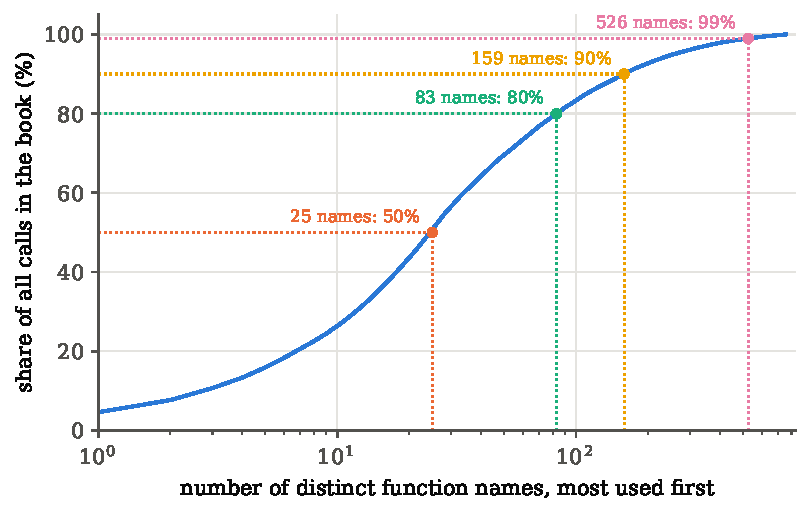
\includegraphics[width=11cm]{figures/chT0/01_census_coverage.pdf}
\caption{The share of all the book's library calls made by the most used names. The horizontal axis counts distinct names, most used first, on a logarithmic scale. Half of all calls use only $\TzNfifty$ names; $\TzNeighty$ names cover $80\%$, $\TzNninety$ cover $90\%$, and the last $1\%$ of calls is spread over hundreds of names that each appear a handful of times.}
\label{T0a:fig:coverage}
\end{figure}

\Cref{T0a:fig:coverage} is the whole answer. Half of all calls use $K_{0.5}=\TzNfifty$ names. Eighty per cent use $K_{0.8}=\TzNeighty$. Ninety per cent use $K_{0.9}=\TzNninety$. The curve then flattens: to reach $99\%$ takes $K_{0.99}=\TzNninetynine$ names, because the last per cent is a long tail of names that each appear once or twice. There are \TzRareNames{} names called three times or fewer in the whole book, and together they make only \TzRareShare\% of the calls. Those are exactly the names it is pointless to learn in advance. Each is used once, for one special job, and the script's comment or the text next to it says what it does.

\paragraph{Example: what the eighty per cent means for one script.} A typical script calls $\TzMedianNames$ distinct library names (the median over all files). Suppose a reader knows the $\TzNeighty$ most used names. How many unfamiliar calls will a script of a hundred calls contain? If the script's calls are drawn like the book's as a whole, each call is one of the known names with probability $c(\TzNeighty)\approx0.8$. The expected number of unknown calls is then
\begin{align*}
  \E[\text{unknown calls}]
  &\eqby{1}\sum_{i=1}^{100}\Prob(\text{call }i\text{ is unknown})
   \eqby{2}100\times\bigl(1-c(\TzNeighty)\bigr)
   \approx 100\times0.2=20 .
\end{align*}
\begin{explain}
  \item The expectation of a count is the sum of the probabilities of the events it counts (each call contributes $1$ if unknown, $0$ if not).
  \item Each call is unknown with probability $1-c(K)$, the share of calls outside the known names.
\end{explain}
Twenty calls sounds like many, but most of them repeat: a script that calls \texttt{hp.anafast} once usually calls it inside a loop or several times with different arguments. In practice the unfamiliar part of a script is one or two library functions, and the comment on that line usually says what they return.

\paragraph{Syntax: the same story, more strongly.} The census also asks, for each piece of syntax, what share of the scripts use it at least once (\cref{T0a:fig:syntax}). Some pieces are everywhere: assignment, function calls, imports, indexing, keyword arguments and tuple unpacking appear in practically every file, \texttt{for} loops in $\TzPctFor\%$, f-strings (a way of putting numbers into text) in $\TzPctFstring\%$, slices in $\TzPctSlice\%$, the definition of a function in $\TzPctDef\%$. Then comes a sharp drop. The \texttt{while} loop appears in $\TzPctWhile\%$ of the scripts, \texttt{try}/\texttt{except} in $\TzPctTry\%$, classes in $\TzPctClass\%$, decorators in $\TzPctDecorator\%$, generators (\texttt{yield}) in none. A course on Python spends weeks on classes, inheritance, generators, exceptions and decorators. The book barely uses them.

\begin{figure}[htbp]
\centering
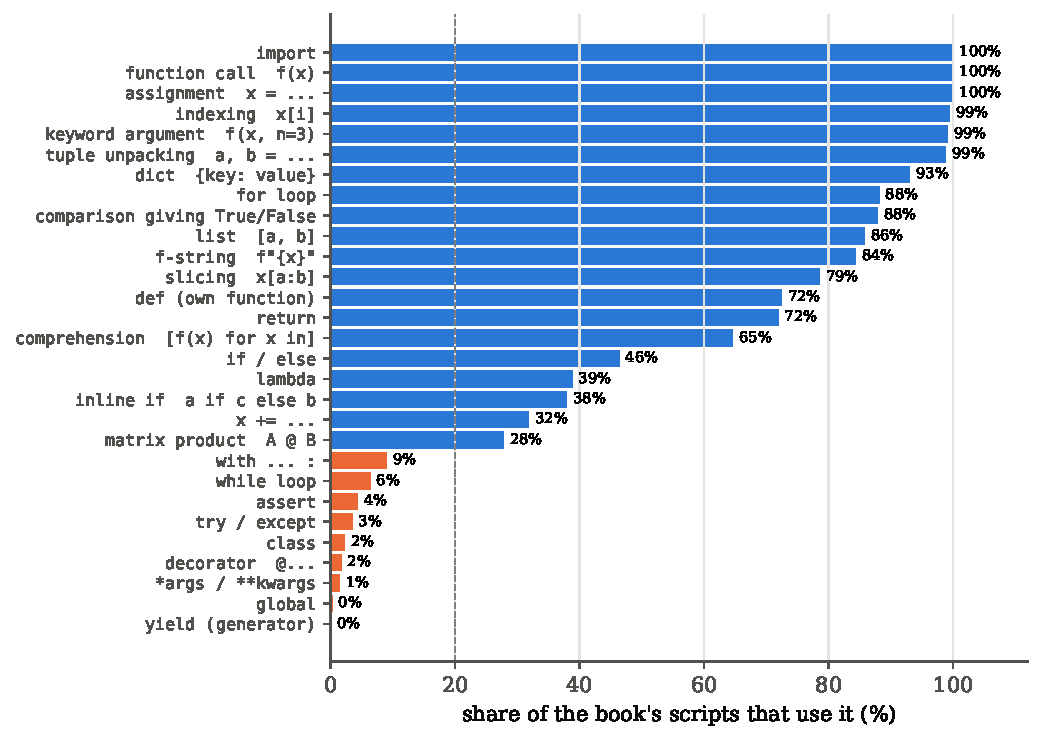
\includegraphics[width=11cm]{figures/chT0/01_census_syntax.pdf}
\caption{For each piece of Python syntax, the share of the book's scripts that use it at least once. Blue bars (at least $20\%$ of the scripts) are the core every reader needs; orange bars are rare and are collected in \cref{T0a:sec:rare}. The dashed line marks $20\%$.}
\label{T0a:fig:syntax}
\end{figure}

\paragraph{Libraries.} The import statements tell the same story. NumPy is imported by $\TzPctNumpy\%$ of the scripts and Matplotlib's plotting module by $\TzPctPlt\%$. SciPy is used by $\TzPctScipy\%$, almost always for one or two functions. healpy, the library for maps on the sphere, appears in $\TzPctHealpy\%$, and CAMB, the cosmology code, in $\TzPctCamb\%$; numba and the multiprocessing module in about $\TzPctNumba\%$ each. By number of calls, NumPy names make $\TzNumpyShare\%$ of all library calls, plotting calls about $\TzPlotShare\%$ and SciPy only $\TzScipyShare\%$: SciPy functions are powerful, so one call does a lot. The rest are Python's own built-in functions, such as \texttt{len}, \texttt{range}, \texttt{print}, and methods of arrays and lists, such as \texttt{x.mean()} or \texttt{results.append(\dots)}.

\Cref{T0a:fig:topcalls} lists the forty most used names, coloured by library. It is worth reading slowly once: together these forty names cover more than half of everything the book's code does, and each of them reappears below with an example.

\begin{figure}[htbp]
\centering
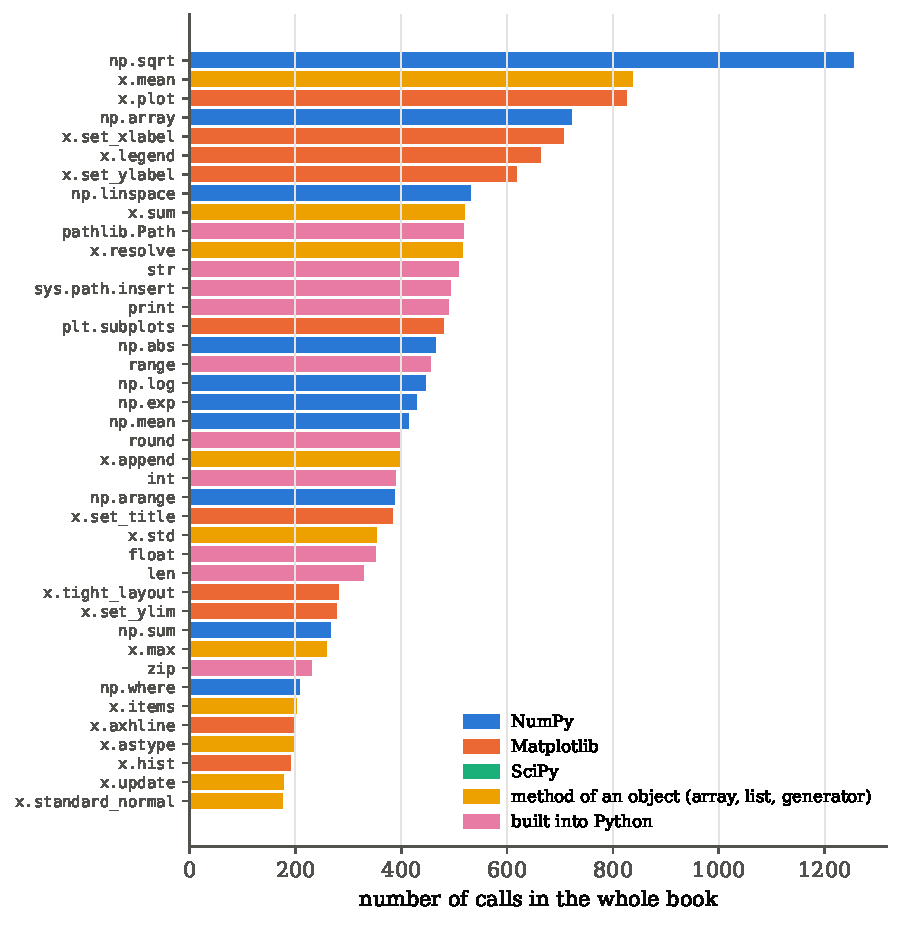
\includegraphics[width=10.5cm]{figures/chT0/01_census_topcalls.pdf}
\caption{The forty most used names in the book's code, by number of calls. \texttt{x.} stands for a method called on some object: \texttt{x.mean} is the mean of an array, \texttt{x.plot} draws on a set of axes, \texttt{x.append} adds an item to a list. Blue are NumPy functions, orange Matplotlib, green SciPy, yellow methods of arrays, lists and random generators, pink Python's built-in functions.}
\label{T0a:fig:topcalls}
\end{figure}

\begin{keyidea}[A small vocabulary does almost everything]
About $\TzNfifty$ names cover half of all the function calls in the book, about $\TzNeighty$ cover $80\%$, and the syntax needed is the core of the language: assignment, calls with keyword arguments, indexing and slicing, \texttt{for} and \texttt{if}, short functions, lists, tuples and dictionaries. Everything else is rare and can be looked up when met.
\end{keyidea}

That vocabulary is best learned in the order in which a reader meets it inside a script, each idea with its minimal syntax, a real excerpt from one of the book's scripts, and the one mistake most often made with it.
\section{Running a script and reading what it prints}
\label{T0a:sec:anatomy}

A script is a recipe for an experiment that the computer carries out. Like a lab procedure, it has a fixed shape: what it is for, what equipment it uses, the measurement itself, and where the results are written down. Every script in the book follows the same shape, so once one script has been read closely, the others look familiar. We read one closely here: \pyname{code/ch02/02_binomial.py}, which checks the binomial distribution of \cref{2a:sec:binomial} by simulation. Its question is: if we repeat a yes/no trial with success probability $p$ a number $n$ of times and count the successes, does the histogram of that count match the binomial formula $\binom nk p^k(1-p)^{n-k}$?

\paragraph{Running it.} From the top directory of the book (the folder \texttt{Notes}), one types in a terminal
\begin{center}
\texttt{python3 code/ch02/02\_binomial.py}
\end{center}
Python reads the file from the top and carries out its lines one after another. When it finishes, two new files exist: the figure \texttt{figures/ch02/02\_binomial.pdf} and the numbers file \texttt{results/ch02/02\_binomial.tex}. The terminal shows what the script chose to print, here two short lines naming those files. The book's own runs were made the same way, on a computing cluster, and the two files copied back. The random numbers are seeded by the script's name (\cref{0a:sec:code}), so the outputs are identical wherever the script runs.

\paragraph{When it fails.} If something goes wrong, Python stops and prints a \newterm{traceback}: a list of the lines that were being executed, innermost last, followed by one line naming the error. The last line is the one to read first. For example, adding an array of three numbers to an array of four numbers stops a script with
\begin{center}
\texttt{ValueError: operands could not be broadcast together with shapes (3,) (4,)}
\end{center}
which says exactly what is wrong: two arrays whose shapes do not fit (\cref{T0a:sec:broadcasting}). The line above it in the traceback gives the file and line number where it happened. Reading the traceback from the bottom up is the single most useful debugging habit.

\begin{figure}[htbp]
\centering
\begin{tikzpicture}[
  blk/.style={draw=accent,rounded corners=2pt,fill=ideabg,align=left,font=\footnotesize,
              text width=5.6cm,minimum height=0.75cm,inner sep=3pt},
  outfile/.style={draw=softgray,rounded corners=2pt,fill=codebg,align=center,font=\footnotesize\ttfamily,
              text width=3.6cm,minimum height=0.75cm},
  ln/.style={font=\scriptsize\ttfamily,softgray,anchor=east},
  arr/.style={->,thick,accent}]
  \node[blk] (doc) at (0,0) {\textbf{docstring}: Question, Computes, Writes};
  \node[blk] (imp) at (0,-1.0) {\textbf{imports}: the \texttt{sys.path} line, numpy, matplotlib, scipy, common};
  \node[blk] (set) at (0,-2.0) {\textbf{settings}: \texttt{setup()}, \texttt{rng = rng\_for(\dots)}, sizes};
  \node[blk] (fun) at (0,-3.0) {\textbf{own functions}: \texttt{def binomial\_by\_trials(\dots)}};
  \node[blk] (cmp) at (0,-4.0) {\textbf{the computation and the figure}: loop over cases};
  \node[blk] (num) at (0,-5.0) {\textbf{the numbers}: \texttt{save\_numbers(\dots)}};
  \node[ln] at (-3.0,0) {1--10};
  \node[ln] at (-3.0,-1.0) {11--15};
  \node[ln] at (-3.0,-2.0) {17--19};
  \node[ln] at (-3.0,-3.0) {21--24};
  \node[ln] at (-3.0,-4.0) {26--52};
  \node[ln] at (-3.0,-5.0) {54--60};
  \node[outfile] (fig) at (5.6,-3.5) {figures/ch02/\\02\_binomial.pdf};
  \node[outfile] (res) at (5.6,-5.0) {results/ch02/\\02\_binomial.tex};
  \draw[arr] (cmp.east) -- (fig.west);
  \draw[arr] (num.east) -- (res.west);
\end{tikzpicture}
\caption{The six blocks of every script in the book, with the line numbers they occupy in \pyname{02_binomial.py}. The two grey boxes are the files the script writes: the chapter text includes the figure and reads its numbers from the second file.}
\label{T0a:fig:anatomy}
\end{figure}

\paragraph{The whole script.} Here it is, all sixty lines.

\pyfile{code/ch02/02_binomial.py}{A complete book script: the binomial distribution by simulation}

We walk through it block by block (\cref{T0a:fig:anatomy}).

\emph{The docstring (lines 1--10).} Text between triple quotes at the top of a file is the file's \newterm{docstring}. Python stores it but does not execute it. Every script in the book states three things there: the \emph{Question} it answers, what it \emph{Computes}, and what it \emph{Writes}. Reading the docstring first tells us what to look for in the rest.

\emph{The imports (lines 11--15).} Line 11 is the same in every script and is explained once below. Lines 12--14 load NumPy under the short name \texttt{np}, Matplotlib's plotting module as \texttt{plt}, and the binomial distribution from SciPy. Line 15 loads four helpers from the book's own module \pyname{common.py}: \pyname{setup} (the figure style), \pyname{savefig} (write a figure into the right folder), \pyname{save_numbers} (write numbers for the text) and \pyname{rng_for} (a random generator seeded by the script's name). What each helper does inside is described in \cref{0a:sec:code}; here it is enough to know what goes in and what comes out.

\emph{The settings (lines 17--19).} \texttt{setup(6.4, 4.6)} sets the figure size in inches and the house style. \texttt{rng = rng\_for("ch02", "02\_binomial")} creates the random generator. Every random number in the script comes from \texttt{rng}. \texttt{reps = 20\_000} fixes the number of repetitions; the underscore only makes the number easier to read.

\emph{The script's own function (lines 21--24).} \texttt{binomial\_by\_trials(n, p, reps)} draws a table of uniform random numbers with \texttt{reps} rows and \texttt{n} columns, marks each entry \texttt{True} when it is below $p$ (a success), and counts the successes in each row. Line 24 does the counting with \texttt{trials.sum(axis=1)}: adding \texttt{True} as $1$ and \texttt{False} as $0$ along each row. Every idea in these four lines (arrays, comparisons that make masks, sums along an axis) appears again in \cref{T0a:sec:numpy}.

\emph{The computation and the figure (lines 26--52).} Line 27 lists six pairs $(n,p)$. Line 28 creates a figure with a $3\times2$ grid of panels. Line 29 walks through the panels and the pairs side by side: for each panel \texttt{ax} and each pair \texttt{(n, p)}, line 30 simulates, line 32 turns the counts into frequencies, and lines 33--34 draw the simulated bars and the exact probabilities as short black marks. Line 43 saves the figure. Lines 46--52 then compute two more checks: a trigger that fires when at least three of four detector layers fire, exactly and by simulation, and the mean and variance of the count.

\emph{The numbers (lines 54--60).} \texttt{save\_numbers} writes the five numbers to \texttt{results/\allowbreak ch02/\allowbreak 02\_binomial.tex}, each as a \LaTeX{} command, for example \verb|\twoaTrigExact|. The chapter text writes that command where the number belongs, so the number in the text is always the one the script printed.

\begin{figure}[htbp]
\centering
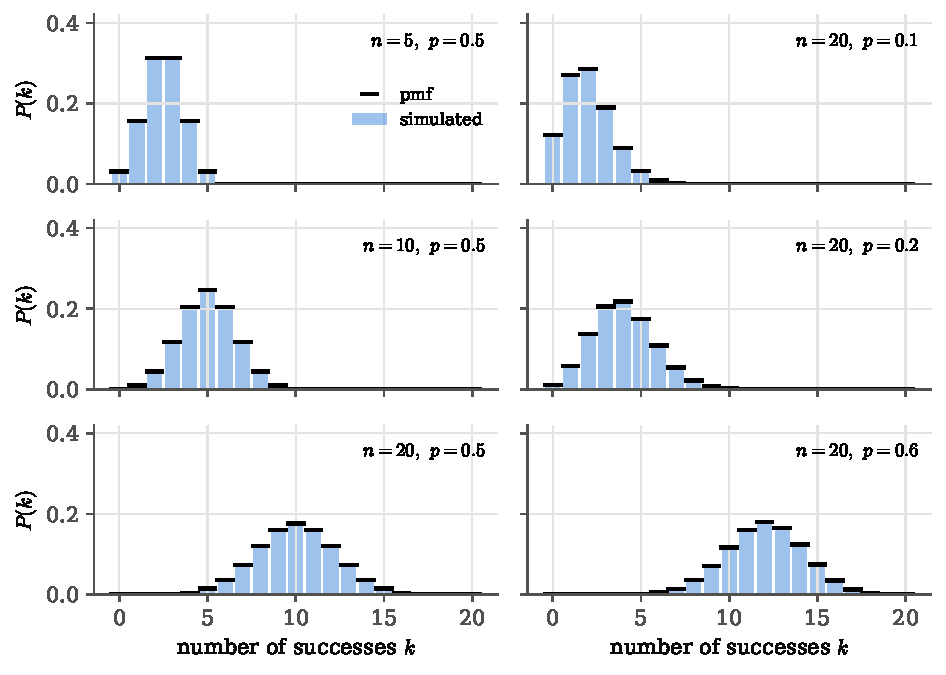
\includegraphics[width=9.5cm]{figures/ch02/02_binomial.pdf}
\caption{What \pyname{02_binomial.py} draws: for six choices of the number of trials $n$ and the success probability $p$, the frequencies of $k$ successes in $20\,000$ simulated experiments (blue bars) and the binomial probabilities (black marks). The left column grows $n$ at $p=0.5$; the right column grows $p$ at $n=20$.}
\label{T0a:fig:binomial-output}
\end{figure}

\paragraph{The one line that is the same everywhere.} Line 11 reads
\begin{center}
\texttt{import sys, pathlib; sys.path.insert(0, str(pathlib.Path(\_\_file\_\_).resolve().parents[1]))}
\end{center}
It looks cryptic, but it is a chain of small steps, each turning one thing into the next. Its job is to tell Python where \pyname{common.py} lives, so that line 15 can import it. Python looks for modules in a list of folders called \texttt{sys.path}, and the folder \texttt{code/} is not on that list by default. So the line computes the path of \texttt{code/} and puts it at the front of the list. For this script, read inside out:
\begin{align*}
  \texttt{\_\_file\_\_}
  &\eqby{1}\texttt{"code/ch02/02\_binomial.py"}\\
  \texttt{pathlib.Path(\_\_file\_\_).resolve()}
  &\eqby{2}\texttt{/\dots/Notes/code/ch02/02\_binomial.py}\\
  \texttt{\dots.parents[0]}
  &\eqby{3}\texttt{/\dots/Notes/code/ch02}\\
  \texttt{\dots.parents[1]}
  &\eqby{4}\texttt{/\dots/Notes/code}\\
  \texttt{sys.path.insert(0, str(\dots))}
  &\eqby{5}\text{put that folder first in the search list.}
\end{align*}
\begin{explain}
  \item Python sets \texttt{\_\_file\_\_} to the path by which the script was started.
  \item \texttt{pathlib.Path} turns the text into a path object, and \texttt{resolve()} makes it a full path from the root of the disk, whichever folder we started from.
  \item \texttt{parents[0]} is the folder that contains the file.
  \item \texttt{parents[1]} is one folder further up: \texttt{code/}, where \pyname{common.py} is.
  \item \texttt{str} turns the path object back into text, and \texttt{insert(0, \dots)} puts it at position $0$, the front, so it is searched first.
\end{explain}
The tour script \pyname{code/chT0/06_python_tour.py} prints the last names of these folders for itself: \texttt{here.parents[0].name} is \texttt{'chT0'} and \texttt{here.parents[1].name} is \texttt{'code'}. Because the path is computed from the script's own location, the script runs correctly whether it is started from \texttt{Notes}, from \texttt{Notes/code}, or from anywhere else. Library files of one chapter used by another (such as \pyname{code/ch07/lib_fields.py}) are reached the same way, with one more \texttt{sys.path.insert} line naming their folder.

\paragraph{Example: reading a printed summary.} Some scripts print a short report as they run. The census script of \cref{T0a:sec:census} prints three lines and keeps them in a text file:

\Tzout{results/chT0/01_census_out.txt}

The first line gives the size of the job (files, lines, calls, distinct names). The second gives $K_{0.5},K_{0.8},K_{0.9},K_{0.99}$ of \cref{T0a:fig:coverage}, in that order. The third gives the long tail. Printing a few such lines, with words next to the numbers, is what makes a script's output readable a month later.

\begin{pitfall}[Never edit a results file by hand]
The files in \texttt{results/} are written by the scripts. If a number in the text looks wrong, the fix is in the script: change it, rerun it, and the text updates itself. A number changed by hand in \texttt{results/} is silently overwritten at the next run, and until then the text disagrees with the code.
\end{pitfall}
\section{Plain Python: values, containers, loops and functions}
\label{T0a:sec:python}

Strip away the libraries and a script is a sequence of small instructions: give a number a name, collect several numbers together, repeat something for each item of a collection, do one thing or another depending on a condition, and package a recipe so that it can be used again. That is the whole of the plain Python the book needs. Every block below was run by \pyname{code/chT0/06_python_tour.py}, and each block shows a few lines of that script followed by exactly what they printed. The helper \texttt{say} prints a line and keeps a copy for the book; many lines use the f-string form \texttt{f"\{x = \}"}, which prints the expression itself followed by its value (\cref{T0a:sec:strings}).

\subsection{Numbers and names}
\label{T0a:sec:numbers}

The line \texttt{n = 20} does not state an equation. It is an instruction: compute the right-hand side and attach the name on the left to the result. The \newterm{assignment} \texttt{n = n + 1} is therefore perfectly sensible: take the current value of \texttt{n}, add one, and attach the name \texttt{n} to the new value.

Python has two kinds of number that matter here. An \newterm{integer} (type \texttt{int}) is a whole number, exact and of any size: a count of events, an index, a number of simulations. A \newterm{float} is a real number stored with about sixteen significant digits (\cref{T0a:sec:trust} says exactly how many and why). \texttt{20} is an integer, \texttt{20.0} and \texttt{0.2} are floats, and \texttt{1.5e-3} means $1.5\times10^{-3}$.

\pyfile[firstline=35,lastline=42,firstnumber=35]{code/chT0/06_python_tour.py}{The tour: numbers and names}
\noindent It prints:
\Tzout{results/chT0/06_numbers.txt}

The operators are \texttt{+ - * /}, \texttt{**} for powers ($2^{10}$ is \texttt{2 ** 10}, never \verb|2^10|, which means something else), \texttt{//} for whole-number division and \texttt{\%} for the remainder. Division with \texttt{/} always gives a float, even for two integers: $20/8=2.5$. Underscores inside a number are ignored, so \texttt{1\_000\_000} is a million written readably. The book uses this everywhere for sizes of simulations: \texttt{reps = 20\_000} in \cref{T0a:sec:anatomy}, \texttt{M = 200\_000} below.

\begin{pitfall}[The caret is not a power]
\texttt{2 ** 10} is $1024$. \verb|2 ^ 10| is $8$: the caret combines the bits of two integers, an operation the book never needs. A formula copied from paper with \verb|^| for powers runs without complaint and gives nonsense.
\end{pitfall}

\subsection{Text and f-strings}
\label{T0a:sec:strings}

Text is a \newterm{string}: characters between quotes, single or double. Strings are used for file names, labels on axes and lines of printed output. Two operations cover most uses. Strings can be joined with \texttt{+}, and single characters or pieces can be taken out by position, exactly as for lists (\cref{T0a:sec:containers}).

\pyfile[firstline=46,lastline=49,firstnumber=46]{code/chT0/06_python_tour.py}{The tour: text}
\noindent It prints:
\Tzout{results/chT0/06_strings.txt}

The operation that the book uses constantly is the \newterm{f-string}: a string with an \texttt{f} before the opening quote, in which anything between curly braces is computed and written into the text. A colon inside the braces sets the format: \texttt{:.3f} means three digits after the decimal point, \texttt{:.2e} scientific notation with two digits after the point, \texttt{:,} thousands separators. Writing \texttt{=} at the end, as in \verb|f"{n = }"|, prints the expression and its value; the tour script uses this for every line it prints.

\pyfile[firstline=53,lastline=57,firstnumber=53]{code/chT0/06_python_tour.py}{The tour: formatting numbers in f-strings}
\noindent It prints:
\Tzout{results/chT0/06_fstrings.txt}

Here is how a real script uses f-strings. \pyname{code/ch01/01_events_as_masks.py} (\cref{1a:sec:events}) sends its numbers to the text, rounding some of them to four digits on the way:

\pyfile[firstline=49,lastline=56,firstnumber=49]{code/ch01/01_events_as_masks.py}{Numbers sent to the text, some formatted by f-strings}

The keys on the left (\texttt{"OneAMaskExA"} and so on) become the names of \LaTeX{} commands. The values are either numbers, which \pyname{save_numbers} formats itself, or strings already formatted with f-strings, such as \verb|f"{pA:.4f}"|, which writes the probability \texttt{pA} with four decimals. Plot labels are f-strings too: line 35 of the binomial script writes \verb|f"$n={n},\\ p={p}$"|, which becomes the label $n=20,\ p=0.2$ in the figure.

\begin{pitfall}[Backslashes in labels]
A backslash inside an ordinary Python string starts a special character: \verb|"\n"| is a new line and \verb|"\t"| a tab. So the \LaTeX{} label \verb|"$\theta$"| arrives as a tab followed by \texttt{heta}. Either double every backslash (\verb|"$\\theta$"|) or put an \texttt{r} before the quote (\verb|r"$\theta$"|), which tells Python to leave backslashes alone. The book's scripts use both forms.
\end{pitfall}

\subsection{Lists, tuples and dictionaries}
\label{T0a:sec:containers}

Three containers hold several values under one name.

A \newterm{list} is an ordered sequence in square brackets, \texttt{[1, 2, 5, 30]}, which can grow. Its items are numbered from $0$, not from $1$, so \texttt{ns[0]} is the first item. Negative positions count from the end: \texttt{ns[-1]} is the last item. A \newterm{slice} \texttt{ns[a:b]} takes the items from position \texttt{a} up to, but not including, position \texttt{b}. \texttt{.append(x)} adds an item at the end. The method \texttt{.append} is called $\TzAppendCalls$ times in the book's code, almost always in one pattern: start with an empty list, and append one result each time round a loop.

\pyfile[firstline=61,lastline=69,firstnumber=61]{code/chT0/06_python_tour.py}{The tour: a list, and the start-empty-then-append pattern}
\noindent It prints:
\Tzout{results/chT0/06_lists.txt}

The rule ``from \texttt{a}, stopping before \texttt{b}'' becomes obvious once positions are pictured as the \emph{gaps between items}, not the items themselves (\cref{T0a:fig:slices}). Then \texttt{ns[1:3]} is everything between gap $1$ and gap $3$: two items. The length of a slice is \texttt{b - a}, and \texttt{ns[:k]} followed by \texttt{ns[k:]} gives back the whole list with nothing repeated and nothing lost.

\begin{figure}[htbp]
\centering
\begin{tikzpicture}[x=1.25cm,y=1cm,
  cell/.style={draw=accent,fill=ideabg,minimum width=1.25cm,minimum height=0.8cm,font=\small\ttfamily}]
  \foreach \v [count=\i from 0] in {1,2,5,30,100} {
    \node[cell] at (\i+0.5,0) {\v};
  }
  \foreach \i in {0,...,5} {
    \draw[softgray] (\i,0.55) -- (\i,0.8);
    \node[font=\footnotesize\ttfamily,accent] at (\i,1.05) {\i};
  }
  \foreach \i/\n in {0/-5,1/-4,2/-3,3/-2,4/-1} {
    \node[font=\footnotesize\ttfamily,fibreorange] at (\i+0.5,-0.75) {\n};
  }
  \node[font=\footnotesize,accent,anchor=east] at (-0.2,1.05) {gaps};
  \node[font=\footnotesize,fibreorange,anchor=east] at (-0.2,-0.75) {from the end};
  \draw[very thick,tangentgreen] (1,-1.25) -- (3,-1.25);
  \draw[tangentgreen] (1,-1.12) -- (1,-1.38);
  \draw[tangentgreen] (3,-1.12) -- (3,-1.38);
  \node[font=\footnotesize\ttfamily,tangentgreen,anchor=west] at (3.2,-1.25) {ns[1:3] = [2, 5]};
\end{tikzpicture}
\caption{The list \texttt{ns = [1, 2, 5, 30, 100]}. Blue numbers mark the gaps between items: a slice \texttt{ns[a:b]} runs from gap \texttt{a} to gap \texttt{b}, so \texttt{ns[1:3]} holds two items. An index \texttt{ns[i]} is the item just after gap \texttt{i}; orange numbers are the negative indices, counting back from the end.}
\label{T0a:fig:slices}
\end{figure}

A \newterm{tuple} is a fixed group of values in round brackets, \texttt{(20, 0.2)}, which cannot be changed after it is made. The book uses tuples to keep things together that belong together, such as the pair $(n,p)$ of a binomial distribution. Its most useful property is \newterm{unpacking}: \texttt{n, p = case} gives one name to each entry. Unpacking works in \texttt{for} loops too, and is used in practically every script.

\pyfile[firstline=73,lastline=78,firstnumber=73]{code/chT0/06_python_tour.py}{The tour: tuples and unpacking}
\noindent It prints:
\Tzout{results/chT0/06_tuples.txt}

A \newterm{dictionary} (\texttt{dict}) is a table that maps \emph{keys} to \emph{values}, written \texttt{\{"H0": 67.36, "ns": 0.9649\}}. A value is fetched by its key, \texttt{fid["H0"]}, not by a position. New entries are added by assignment, \texttt{fid["tau"] = 0.0544}, and \texttt{.items()} walks through the (key, value) pairs.

\pyfile[firstline=82,lastline=87,firstnumber=82]{code/chT0/06_python_tour.py}{The tour: a dictionary}
\noindent It prints:
\Tzout{results/chT0/06_dicts.txt}

All three containers appear together in the binomial script of \cref{T0a:sec:anatomy}, lines 27--30: a list of tuples \texttt{cases = [(5, 0.5), (10, 0.5), \dots]}, walked through with unpacking, \texttt{for ax, (n, p) in zip(\dots)}. The dictionary \texttt{\{...\}} handed to \pyname{save_numbers} on line 54 is the commonest dictionary in the book. A slightly richer use is in \pyname{code/ch03/01_sampling_distribution.py} (\cref{3a:sec:sampling-python}), which compares four ways of estimating $g$ from ten readings:

\pyfile[firstline=27,lastline=37,firstnumber=27]{code/ch03/01_sampling_distribution.py}{A dictionary of estimators, and a dictionary built from it}

The dictionary \texttt{est} maps a name (a string) to an array of $200\,000$ estimates, one per simulated experiment. Line 37 builds a second dictionary from the first: for every key \texttt{k} and value \texttt{v}, the standard deviation of \texttt{v}. That one-line construction is a \emph{comprehension} (\cref{T0a:sec:control}).

\paragraph{Example: why a dictionary and not a list?} The four estimators could be kept in a list, \texttt{[mean, median, midrange, first]}. Then the standard deviation of the median would be \texttt{sd[1]}, and anyone reading the code must remember that position $1$ is the median. With a dictionary it is \texttt{sd["sample median"]}: the code says what it means, and adding a fifth estimator does not shift the positions of the others. The rule of thumb is: a list when the items are of the same kind and their order matters (a sequence of sizes $N$), a dictionary when each item has a name (estimators, parameters, numbers for the text).

\begin{pitfall}[Counting from zero]
The first item is \texttt{x[0]} and the last is \texttt{x[len(x) - 1]}, also written \texttt{x[-1]}. \texttt{x[len(x)]} does not exist and stops the script with \texttt{IndexError}. When a formula on paper runs over $i=1,\dots,N$, the code runs over \texttt{i = 0, ..., N-1}.
\end{pitfall}

\subsection{Doing things repeatedly, and conditionally}
\label{T0a:sec:control}

A \texttt{for} loop repeats a block of lines once for each item of a collection. The block is marked by \newterm{indentation}: the lines that belong to the loop are shifted to the right by four spaces, and the first line that is not shifted is the first line after the loop. Python has no \texttt{end} statement; the indentation \emph{is} the structure.

\texttt{range(n)} produces the integers $0,1,\dots,n-1$ (\texttt{n} numbers, stopping before \texttt{n}), and \texttt{range(a, b)} those from \texttt{a} up to \texttt{b - 1}. \texttt{enumerate(xs)} gives the position together with each item, and \texttt{zip(xs, ys)} walks two collections side by side.

\pyfile[firstline=91,lastline=98,firstnumber=91]{code/chT0/06_python_tour.py}{The tour: three kinds of for loop}
\noindent It prints:
\Tzout{results/chT0/06_loops.txt}

An \texttt{if} statement runs a block only when a condition is true. \texttt{elif} (``else if'') adds further conditions, tried in order, and \texttt{else} catches everything left. Conditions are comparisons (\texttt{<}, \texttt{<=}, \texttt{==} for ``is equal to'', \texttt{!=} for ``is not equal to'') joined by \texttt{and}, \texttt{or}, \texttt{not}.

\pyfile[firstline=102,lastline=110,firstnumber=102]{code/chT0/06_python_tour.py}{The tour: if, elif, else}
\noindent It prints:
\Tzout{results/chT0/06_ifs.txt}

Both appear together in the dice script of \cref{1a:sec:events}, which colours the $36$ outcomes of two dice according to the two events ``first die even'' and ``sum at least $9$'':

\pyfile[firstline=62,lastline=73,firstnumber=62]{code/ch01/01_events_as_masks.py}{Two nested loops and a three-way condition}

Lines 62--63 are two loops, one inside the other: for each value \texttt{i} of the first die, for each value \texttt{j} of the second, so the inner block runs $6\times6=36$ times. Line 64 computes two true/false values. Lines 66--71 choose a colour: both events (green), only $A$ (blue), only $B$ (orange), and otherwise the white set on line 65 stays. Line 72 draws one square.

A \texttt{while} loop repeats as long as a condition holds, for when the number of repetitions is not known in advance. It is rare in the book ($\TzPctWhile\%$ of the scripts). A typical use is accept--reject sampling (\cref{ch:06}): keep drawing until enough draws have been accepted. \pyname{code/ch03/10_angular_ml.py} (\cref{3b:sec:newton}) does exactly that:

\pyfile[firstline=27,lastline=35,firstnumber=27]{code/ch03/10_angular_ml.py}{Draw until there are enough: a while loop}

Line 31 says: while fewer than \texttt{size} values have been collected, draw another batch of $2\times$\texttt{size} candidates, keep those that pass the test (line 33), and add them to the collection (line 34). Line 35 returns exactly \texttt{size} of them.

A \newterm{comprehension} is a loop that builds a list (or a dictionary) in one line: \texttt{[k ** 2 for k in range(5)]} is the list of the squares of $0,\dots,4$. An \texttt{if} at the end keeps only some items. The same construction inside \texttt{sum(\dots)} or \texttt{max(\dots)} needs no brackets.

\pyfile[firstline=142,lastline=148,firstnumber=142]{code/chT0/06_python_tour.py}{The tour: comprehensions}
\noindent It prints:
\Tzout{results/chT0/06_comprehensions.txt}

Comprehensions are in $\TzPctComp\%$ of the scripts. Line 37 of the sampling-distribution excerpt above, \verb|{k: v.std(ddof=1) for k, v in est.items()}|, is one. A one-line \texttt{if} also exists for values: \texttt{a if condition else b}. It is how the book's code writes a default, as in \texttt{rng = np.random.default\_rng() if rng is None else rng}.

\paragraph{Example: the same sum three ways.} The sum $\sum_{k=1}^{5}k$ is computed by an explicit loop in the tour (\texttt{total = 15}). With a comprehension it is \texttt{sum(k for k in range(1, 6))}. With NumPy (\cref{T0a:sec:numpy}) it is \texttt{np.arange(1, 6).sum()}. All three give $15$. The loop is the clearest; the NumPy form is the fastest for long sums, by a factor of about $\TzSpeedup$ for a million terms (\cref{T0a:sec:vectorise}).

\begin{pitfall}[Indentation is part of the program]
Moving a line four spaces to the left takes it out of the loop: it then runs once, after the loop, instead of once per item. Python cannot warn about this, because both versions are valid programs. When a result looks like ``only the last case was used'', check the indentation of the line that stores the result.
\end{pitfall}

\subsection{Functions}
\label{T0a:sec:functions}

A \newterm{function} packages a recipe with inputs and outputs, so that it can be used many times and read once. It starts with \texttt{def}, its name and its inputs (the \newterm{parameters}) in brackets; the indented block is the recipe; \texttt{return} hands back the result. A string on the first line of the block is the function's docstring. Parameters can have \newterm{default values}, used when the caller does not give them; and a caller can give any parameter by name, as a \newterm{keyword argument}, in any order. To return several results, a function returns them separated by commas, which makes a tuple, and the caller unpacks it.

\pyfile[firstline=123,lastline=138,firstnumber=123]{code/chT0/06_python_tour.py}{The tour: two functions and a lambda}
\noindent It prints:
\Tzout{results/chT0/06_functions.txt}

The first two lines call \texttt{gaussian(x, mu=0.0, sigma=1.0)}: once with both defaults, once giving \texttt{sigma} by name and leaving \texttt{mu} at its default. The third calls \texttt{mean\_and\_error}, which returns two values, unpacked into \texttt{m, e}. The last line uses a \newterm{lambda}: a one-line function without a name, \texttt{lambda t: t ** 2}, convenient when a function is needed only once, as an argument to another function.

Every one of these features is in daily use in the book. The log-likelihood of the decay-time example (\cref{3b:sec:curv-python}) is a two-line function, and the function whose root gives the likelihood interval is a lambda:

\pyfile[firstline=27,lastline=40,firstnumber=27]{code/ch03/09_mle_decay.py}{A function, and lambdas handed to SciPy}

Line 29 is the whole recipe: $\ln\Like(\tau)=-n\ln\tau-\sum_i t_i/\tau$ for decay times $t_i$, with \texttt{len(t)} giving $n$ and \texttt{t.sum()} the sum. Line 35 hands a lambda to SciPy's minimiser: ``the function of \texttt{s} that returns minus the log-likelihood at \texttt{s}''. Line 38 builds the function whose zeros are the points where $\ln\Like$ has dropped by $\tfrac12$ from its maximum, and lines 39--40 find those zeros (\cref{T0a:sec:scipy}).

Library functions in the book use defaults and keyword arguments to stay flexible. The Gaussian-field simulator of \cref{7a:sec:recipe} begins

\pyfile[firstline=45,lastline=53,firstnumber=45]{code/ch07/lib_fields.py}{Defaults and keyword arguments in a library function}

The parameters \texttt{d}, \texttt{rng} and \texttt{nsim} have defaults ($2$ dimensions, no generator given, one field), so the simplest call is \texttt{gaussian\_field(P, N, L)}, and a three-dimensional batch of fields is \texttt{gaussian\_field(P, N, L, d=3, nsim=100, rng=rng)}. The words after the colons (\texttt{N: int}, \texttt{L: float}) are \newterm{type hints}: notes for the reader saying what kind of value is expected. Python ignores them.

\begin{figure}[htbp]
\centering
\begin{tikzpicture}[
  fn/.style={draw=accent,thick,rounded corners=3pt,fill=ideabg,minimum width=4.6cm,minimum height=2.0cm,align=center,font=\small},
  inp/.style={font=\footnotesize\ttfamily,anchor=east},
  arr/.style={->,thick,accent}]
  \node[fn] (f) at (0,0) {\texttt{def mean\_and\_error(x):}\\[2pt] \footnotesize mean and standard error\\ \footnotesize of the readings \texttt{x}};
  \node[inp] (a) at (-3.6,0.5) {np.array([9.80, \dots])};
  \node[inp,softgray] (b) at (-3.6,-0.5) {(no other inputs)};
  \draw[arr] (a.east) -- (f.west |- a.east);
  \node[font=\footnotesize\ttfamily,anchor=west] (o1) at (3.6,0.45) {9.800};
  \node[font=\footnotesize\ttfamily,anchor=west] (o2) at (3.6,-0.45) {0.032};
  \draw[arr] (f.east |- o1.west) -- (o1.west);
  \draw[arr] (f.east |- o2.west) -- (o2.west);
  \node[font=\footnotesize,anchor=west,softgray] at (4.9,0.45) {$\to$ \texttt{m}};
  \node[font=\footnotesize,anchor=west,softgray] at (4.9,-0.45) {$\to$ \texttt{e}};
  \node[font=\footnotesize,align=center] at (0,-1.6) {\texttt{m, e = mean\_and\_error(readings)}};
\end{tikzpicture}
\caption{A function as a box with a name: an array of readings goes in, two numbers come out as a tuple, and the caller gives each a name by unpacking. Nothing inside the box is visible to the caller except what \texttt{return} hands back.}
\label{T0a:fig:function}
\end{figure}

\paragraph{Example: why a function at all?} The binomial script of \cref{T0a:sec:anatomy} simulates the binomial count three times: for the six panels (line 30), for the trigger (line 48) and for the moments (line 52). Without the function \texttt{binomial\_by\_trials}, its two lines would be written three times, and a correction (say, \texttt{<} instead of \texttt{<=}) would have to be made in three places. With the function, it is made once. This is the reason almost three quarters of the scripts ($\TzPctDef\%$) define at least one function of their own.

\begin{pitfall}[A function that forgets to return]
A function without a \texttt{return} line returns the special value \texttt{None}. The mistake looks like this: the last line computes the answer, \texttt{chi2 = np.sum(r ** 2)}, but never returns it. The caller then gets \texttt{None}, and the error appears later, somewhere else, as \texttt{TypeError: unsupported operand type(s) \dots{} 'NoneType'}. When that word appears in an error message, look for a missing \texttt{return}.
\end{pitfall}

\subsection{Modules and imports}
\label{T0a:sec:imports}

A \newterm{module} is a file of Python code whose functions can be used elsewhere. \texttt{import numpy as np} loads the module \texttt{numpy} and calls it \texttt{np} inside the script, so its square root is \texttt{np.sqrt}. \texttt{from scipy import stats} loads one part of SciPy under its own name, and \texttt{from math import comb} loads a single function. The book's short names are fixed: \texttt{np} for NumPy, \texttt{plt} for Matplotlib's plotting module, \texttt{hp} for healpy.

\pyfile[firstline=152,lastline=157,firstnumber=152]{code/chT0/06_python_tour.py}{The tour: imports}
\noindent It prints:
\Tzout{results/chT0/06_imports.txt}

The book's own modules (\pyname{common.py}, \pyname{camb_fiducial.py} and the \pyname{lib_*.py} files of each chapter) are imported the same way once their folder is on \texttt{sys.path} (\cref{T0a:sec:anatomy}). One more construction appears at the bottom of a few of them. \pyname{code/camb_fiducial.py} ends with

\pyfile[firstline=40,lastline=41,firstnumber=40]{code/camb_fiducial.py}{Run main() only when the file is started as a script}

Python sets the name \texttt{\_\_name\_\_} to \texttt{"\_\_main\_\_"} in the file that was started, and to the module's own name in a file that was imported. So \texttt{python3 code/camb\_fiducial.py} computes and saves the CAMB spectra, while \texttt{from camb\_fiducial import load\_fiducial} in another script only makes the function available, without running anything.
\section{NumPy: computing with whole arrays}
\label{T0a:sec:numpy}

A physicist writes $\chi^2=\sum_i (d_i-m_i)^2/\sigma_i^2$ without thinking about the order in which the terms are added. The formula is about whole vectors: the data vector $\data$, the model vector $\bm m$, the vector of errors. NumPy lets code be written the same way. Its central object is the \newterm{array}: a block of numbers, all of the same kind, laid out in a grid of one or more dimensions, on which arithmetic acts element by element. \texttt{(d - m) / s} is the vector of normalised residuals, and \texttt{np.sum(((d - m) / s) ** 2)} is $\chi^2$. NumPy names make $\TzNumpyShare\%$ of all library calls in the book, and NumPy is imported by $\TzPctNumpy\%$ of the scripts: this section is the heart of the toolkit. The printed lines below come from \pyname{code/chT0/07_numpy_tour.py}.

\subsection{Arrays, shape and type}
\label{T0a:sec:arrays}

An array is made from a list with \texttt{np.array([\dots])}, or directly by a function that fills it: \texttt{np.zeros}, \texttt{np.ones}, \texttt{np.full}, \texttt{np.arange}, \texttt{np.linspace}, or a random generator. Three attributes describe it. Its \newterm{shape} is a tuple giving the length along each dimension: \texttt{(4,)} for four readings, \texttt{(2, 3)} for two rows of three. \texttt{ndim} is the number of dimensions, and \texttt{dtype} the kind of number stored, almost always \texttt{float64} (a real number in double precision) or \texttt{int64} (a whole number). Arithmetic and functions such as \texttt{np.sqrt}, \texttt{np.exp}, \texttt{np.log} act on every element.

\Tzout{results/chT0/07_arrays.txt}

Three ways of making evenly spaced numbers need to be told apart, because they are used constantly. \texttt{np.arange(a, b, step)} starts at \texttt{a} and adds \texttt{step} until it reaches \texttt{b}, which it does \emph{not} include; it is meant for integers. \texttt{np.linspace(a, b, n)} gives \texttt{n} points from \texttt{a} to \texttt{b} \emph{including} both ends; it is the right choice for a grid of real numbers, such as the $x$ values at which a density is plotted. \texttt{np.logspace(p, q, n)} gives \texttt{n} points from $10^p$ to $10^q$, evenly spaced in the logarithm, and \texttt{np.geomspace(a, b, n)} the same between \texttt{a} and \texttt{b} themselves; they are the right choice for sample sizes, scales and frequencies that span several decades.

\paragraph{Example: how many points, and what spacing?} A grid of $\theta$ from $0$ to $1$ with steps of $0.1$ has eleven points, $0,0.1,\dots,1$. With \texttt{np.linspace(0, 1, 11)} the spacing is
\begin{align*}
  \Delta\theta
  &\eqby{1}\frac{b-a}{n-1}
   =\frac{1-0}{11-1}=0.1 ,
\end{align*}
\begin{explain}
  \item $n$ points with both ends included leave $n-1$ gaps between them.
\end{explain}
and the last point is exactly $1$. With \texttt{np.arange(0, 1, 0.1)} one gets only ten points, stopping at $0.9$; and because $0.1$ is not exactly representable in binary (\cref{T0a:sec:trust}), \texttt{np.arange} with a fractional step can occasionally include or exclude the end by rounding. Hence the rule: \texttt{arange} for integers, \texttt{linspace} for real grids.

\subsection{Indexing and slicing}
\label{T0a:sec:indexing}

Indexing an array works like indexing a list (\cref{T0a:fig:slices}), with one addition: an array with several dimensions takes one index per dimension, separated by commas. \texttt{A[1, 2]} is the element in row $1$, column $2$ (both counted from $0$). A colon on its own means ``all of this dimension'', so \texttt{A[:, 0]} is the first column and \texttt{A[1]} (or \texttt{A[1, :]}) the second row. A slice \texttt{a:b:step} can take every second or third element, and \texttt{::-1} reverses.

\Tzout{results/chT0/07_indexing.txt}

The book stores many repetitions of an experiment as the \emph{rows} of a two-dimensional array: one row per simulated experiment, one column per reading. Then \texttt{x[:, 0]} is ``the first reading of every experiment'', which is how the sampling-distribution script of \cref{3a:sec:sampling-python} builds its fourth estimator (line 34 of the excerpt in \cref{T0a:sec:containers}).

\subsection{Masks: selecting by a condition}
\label{T0a:sec:masks}

A comparison between an array and a number, such as \texttt{x > 0}, does not give one \texttt{True} or \texttt{False}. It gives an array of them, one per element: a \newterm{boolean mask}. A mask can do three things. Used as an index, \texttt{x[m]} keeps only the elements where the mask is \texttt{True}. Summed, \texttt{m.sum()} counts the \texttt{True} entries, because \texttt{True} counts as $1$ and \texttt{False} as $0$. Averaged, \texttt{m.mean()} is the fraction of \texttt{True} entries, which is how a simulated probability is computed. Masks combine with \texttt{\&} (and), \texttt{|} (or) and \texttt{\textasciitilde} (not). \texttt{np.where(m, a, b)} takes \texttt{a} where the mask is true and \texttt{b} elsewhere.

\Tzout{results/chT0/07_masks.txt}

Masks are the bridge between probability and code, and the very first script of \cref{ch:01} is built on them (\cref{1a:sec:events}). An event is a set of outcomes; in a simulation, an event \emph{is} a mask over the simulated outcomes:

\pyfile[firstline=20,lastline=40,firstnumber=20]{code/ch01/01_events_as_masks.py}{Events as boolean masks over $100\,000$ simulated rolls of two dice}

Lines 24--25 roll two dice $N=100\,000$ times: \texttt{rng.integers(1, 7, size=N)} draws integers from $1$ to $6$ (the upper end $7$ is excluded, as for \texttt{range}). Line 28 is the event ``first die even'' as a mask: \texttt{d1 \% 2 == 0} is \texttt{True} where the remainder on division by $2$ is zero. Lines 32--34 are intersection, union and complement, written \texttt{\&}, \texttt{|}, \texttt{\textasciitilde}. Line 40 checks the inclusion--exclusion identity $|A\cup B|=|A|+|B|-|A\cap B|$ on the counts, each count being a \texttt{.sum()} of a mask. The frequency of $A$ is then \texttt{A.mean()}, which estimates $\Prob(A)$.

\paragraph{Example: a probability as the mean of a mask.} Why is \texttt{A.mean()} an estimate of $\Prob(A)$? Write $I_i=1$ if roll $i$ lies in $A$ and $I_i=0$ otherwise; the mask \texttt{A} is the array $(I_1,\dots,I_N)$. Then
\begin{align*}
  \texttt{A.mean()}
  &\eqby{1}\frac1N\sum_{i=1}^N I_i
   \eqby{2}\frac{\#\{i:\ \text{roll } i\in A\}}{N},
  &
  \E[\texttt{A.mean()}]
  &\eqby{3}\frac1N\sum_{i=1}^N\E[I_i]
   \eqby{4}\Prob(A) .
\end{align*}
\begin{explain}
  \item \texttt{.mean()} adds the entries and divides by their number, with \texttt{True} counted as $1$.
  \item The sum of the indicators counts the rolls that land in $A$.
  \item The expectation of a sum is the sum of the expectations.
  \item Each indicator has expectation $1\cdot\Prob(A)+0\cdot(1-\Prob(A))=\Prob(A)$.
\end{explain}
So the mean of a mask is the relative frequency, an unbiased estimate of the probability, with the binomial standard error $\sqrt{\Prob(A)(1-\Prob(A))/N}$ (\cref{T0a:sec:trust}).

\begin{pitfall}[\texttt{and} is not \texttt{\&}]
For masks, write \texttt{(x > 0) \& (x < 1)}, with the brackets. The word \texttt{and} works only for single \texttt{True}/\texttt{False} values and stops with \texttt{ValueError: The truth value of an array with more than one element is ambiguous}. Without the brackets, \texttt{x > 0 \& x < 1} is read as \texttt{x > (0 \& x) < 1}, because \texttt{\&} binds more tightly than \texttt{>}.
\end{pitfall}

\subsection{Broadcasting: arrays of different shapes}
\label{T0a:sec:broadcasting}

\texttt{g * 2} multiplies every element of \texttt{g} by $2$: the single number is ``stretched'' to the shape of the array. NumPy generalises this to arrays of different shapes, and the generalisation, called \newterm{broadcasting}, is what lets the book write tables of pairs without loops.

\begin{workdef}[broadcasting]
Two arrays can be combined element by element when their shapes are compatible. Compare the shapes from the right (the last dimension first). Two lengths are compatible if they are equal or if one of them is $1$ \unpack{a length-$1$ dimension is copied as often as needed}. A missing dimension on the left counts as length $1$. The result has, in each dimension, the larger of the two lengths.
\end{workdef}

The tool for making a length-$1$ dimension on purpose is \texttt{None} as an index. If \texttt{r} has shape \texttt{(3,)}, then \texttt{r[:, None]} has shape \texttt{(3, 1)} (a column) and \texttt{r[None, :]} has shape \texttt{(1, 3)} (a row). Their difference has shape \texttt{(3, 3)}, and its entry $(i,j)$ is $r_i-r_j$ (\cref{T0a:fig:broadcast}).

\Tzout{results/chT0/07_broadcasting.txt}

\begin{figure}[htbp]
\centering
\begin{tikzpicture}[x=0.75cm,y=0.75cm,
  c/.style={draw=accent,fill=ideabg,minimum size=0.75cm,font=\footnotesize\ttfamily,inner sep=0},
  g/.style={draw=softgray,dashed,fill=white,minimum size=0.75cm,font=\footnotesize\ttfamily,text=softgray,inner sep=0}]
  \foreach \v [count=\i from 0] in {0,1,3} { \node[c] at (0,-\i) {\v}; }
  \foreach \v [count=\i from 0] in {0,1,3} { \node[g] at (1,-\i) {\v}; \node[g] at (2,-\i) {\v}; }
  \node[font=\footnotesize,align=center,anchor=south] at (1,0.6) {\texttt{r[:, None]}\\ $(3,1)\to(3,3)$};
  \node at (3.25,-1) {$-$};
  \foreach \v [count=\j from 0] in {0,1,3} { \node[c] at (4.5+\j,0) {\v}; }
  \foreach \v [count=\j from 0] in {0,1,3} { \node[g] at (4.5+\j,-1) {\v}; \node[g] at (4.5+\j,-2) {\v}; }
  \node[font=\footnotesize,align=center,anchor=south] at (5.5,0.6) {\texttt{r[None, :]}\\ $(1,3)\to(3,3)$};
  \node at (8.0,-1) {$=$};
  \foreach \row [count=\i from 0] in {{0,-1,-3},{1,0,-2},{3,2,0}} {
    \foreach \v [count=\j from 0] in \row { \node[c,fill=takebg] at (9.25+\j,-\i) {\v}; }
  }
  \node[font=\footnotesize,align=center,anchor=south] at (10.25,0.6) {all differences\\ $r_i-r_j$};
\end{tikzpicture}
\caption{Broadcasting a column against a row. The column of shape $(3,1)$ is copied sideways and the row of shape $(1,3)$ is copied downwards (dashed copies are never actually stored), so the difference is the full $3\times3$ table of $r_i-r_j$.}
\label{T0a:fig:broadcast}
\end{figure}

The book uses exactly this to build covariance matrices that depend on the distance between two points. The correlated one-dimensional field of \cref{6b:sec:cholesky} has covariance $C_{ij}=e^{-|x_i-x_j|/\ell}$ between grid points $x_i$ and $x_j$, and the whole $200\times200$ matrix is one line:

\pyfile[firstline=38,lastline=42,firstnumber=38]{code/ch06/23_cholesky_field.py}{A covariance matrix from all pairwise distances, by broadcasting}

Line 39 sets the sizes and line 40 makes the $200$ grid positions. In line 41, \texttt{xg[:, None] - xg[None, :]} is the $200\times200$ table of differences, \texttt{np.abs} takes their absolute values, and the exponential is applied to every entry. Line 42 factorises the matrix (\cref{T0a:sec:linalg}).

\paragraph{Example: when shapes do not fit.} Adding \texttt{r} of shape \texttt{(3,)} to \texttt{np.ones(4)} of shape \texttt{(4,)} compares the last lengths, $3$ and $4$. They differ and neither is $1$, so the operation is refused with the error quoted in \cref{T0a:sec:anatomy}. The error is a friend: NumPy refuses to guess what was meant. The dangerous case is the opposite one, when the shapes \emph{do} fit but not in the way intended. Subtracting a vector of $3$ column means from a $3\times3$ matrix, \texttt{A - A.mean(axis=0)}, subtracts each column's mean from its column, as intended; \texttt{A - A.mean(axis=1)} subtracts the \emph{row} means from the \emph{columns}, also without complaint. For square arrays, only the numbers reveal the mistake. Writing \texttt{A.mean(axis=1, keepdims=True)}, which keeps the reduced dimension with length $1$ (shape $(3,1)$), makes the intention explicit.

\subsection{Vectorisation: why loops are avoided}
\label{T0a:sec:vectorise}

Python can of course compute $\chi^2$ with a loop over the data points. The question is how much slower it is, and why. \pyname{code/chT0/02_vectorise.py} computes the same $\chi^2$ in both ways for $N$ from $10$ to $10^6$ or $10^7$:

\pyfile[firstline=19,lastline=29,firstnumber=19]{code/chT0/02_vectorise.py}{The same sum, one element at a time and as one array expression}

For $N=10^6$ the loop takes $\TzLoopMillion$\,s and the array expression $\TzVecMillionMs$\,ms, a factor of $\TzSpeedup$; the two answers agree to a relative difference of $\TzVecRelDiff$, which is rounding error from adding the terms in a different order (\cref{T0a:fig:vectorise}).

\begin{figure}[htbp]
\centering
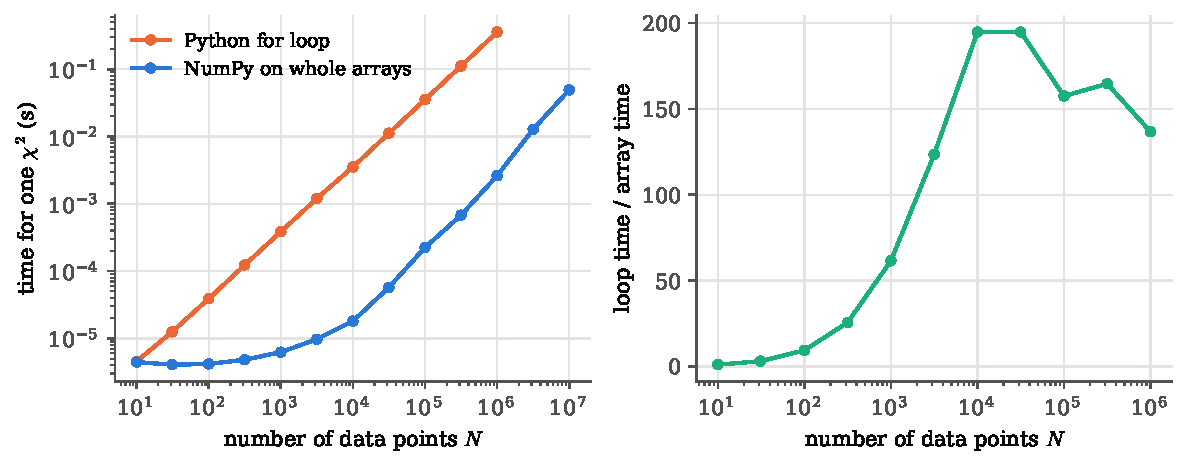
\includegraphics[width=12cm]{figures/chT0/02_vectorise.pdf}
\caption{Left: the time to compute one $\chi^2$ of $N$ data points with a Python loop (orange) and with one NumPy expression (blue). Both grow in proportion to $N$, but the loop pays far more per point. Right: the ratio of the two times, close to $1$ for a handful of points and about a hundred for large $N$.}
\label{T0a:fig:vectorise}
\end{figure}

\paragraph{Where the factor comes from.} Both versions do the same arithmetic, so the difference must be in the overhead around it. In the loop, Python handles each number as a separate object: it looks up \texttt{d[i]}, checks its type, creates a new object for each intermediate result, and only then does the floating-point operation, which itself takes a nanosecond or less. In the array expression, Python is consulted once per \emph{array}; the loop over elements runs inside NumPy's compiled code, on numbers stored side by side in memory. A simple cost model makes this quantitative. Let each version cost a fixed overhead plus a cost per element, $T_{\rm loop}=o_{\rm loop}+c_{\rm loop}N$ and $T_{\rm vec}=o_{\rm vec}+c_{\rm vec}N$. Then
\begin{align*}
  \frac{T_{\rm loop}}{T_{\rm vec}}
  &\eqby{1}\frac{o_{\rm loop}+c_{\rm loop}N}{o_{\rm vec}+c_{\rm vec}N}
   \;\xrightarrow{\;N\to\infty\;}\;\frac{c_{\rm loop}}{c_{\rm vec}}
   \eqby{2}\frac{\TzLoopNsPerElem\ \text{ns}}{\TzVecNsPerElem\ \text{ns}}
   \approx\TzSpeedup .
\end{align*}
\begin{explain}
  \item For large $N$ the overheads are negligible next to the terms proportional to $N$.
  \item The measured costs per element at $N=10^6$: the total times divided by $10^6$.
\end{explain}
For $N=10$ the ratio is about $\TzSpeedupSmall$: both versions are dominated by the fixed overhead of a function call, and vectorising buys nothing. The lesson is practical: a loop over a few dozen cases (six binomial panels, ten sample sizes) is fine and often clearest; a loop over a million data points or simulated values is written as an array expression.

\subsection{Reductions along an axis}
\label{T0a:sec:axis}

A \newterm{reduction} turns many numbers into fewer: \texttt{sum}, \texttt{mean}, \texttt{std}, \texttt{var}, \texttt{min}, \texttt{max}, \texttt{median}, \texttt{percentile}. On a two-dimensional array, the keyword \texttt{axis} says which dimension is reduced, that is, which dimension \emph{disappears}. With experiments in rows and readings in columns, \texttt{E.mean(axis=1)} averages along each row and leaves one mean per experiment; \texttt{E.mean(axis=0)} averages down each column and leaves one mean per reading slot; with no \texttt{axis}, all numbers are averaged (\cref{T0a:fig:axis}).

\Tzout{results/chT0/07_reductions.txt}

\begin{figure}[htbp]
\centering
\begin{tikzpicture}[x=0.8cm,y=0.6cm,
  c/.style={draw=accent,fill=ideabg,minimum width=0.8cm,minimum height=0.6cm,font=\scriptsize\ttfamily,inner sep=0},
  r/.style={draw=tangentgreen,fill=takebg,minimum width=0.8cm,minimum height=0.6cm,font=\scriptsize\ttfamily,inner sep=0}]
  \foreach \row [count=\i from 0] in {{9.80,9.71,9.86,9.83},{9.79,9.85,9.77,9.81},{9.90,9.74,9.82,9.80}} {
    \foreach \v [count=\j from 0] in \row { \node[c] at (\j,-\i) {\v}; }
  }
  \draw[->,thick,fibreorange] (-0.5,0.75) -- (3.5,0.75) node[right,font=\footnotesize] {\texttt{axis=1}: along each row};
  \foreach \v [count=\i from 0] in {9.800,9.805,9.815} { \node[r] at (5.2,-\i) {\v}; }
  \draw[->,thick,formblue] (-0.85,0.3) -- (-0.85,-2.3);
  \node[font=\footnotesize,formblue,anchor=east,align=right] at (-1.0,-1) {\texttt{axis=0}:\\ down each\\ column};
  \foreach \v [count=\j from 0] in {9.830,9.767,9.817,9.813} { \node[r] at (\j,-3.4) {\v}; }
  \node[font=\footnotesize,anchor=west] at (4.6,-3.4) {\texttt{E.mean(axis=0)}, shape $(4,)$};
  \node[font=\footnotesize,anchor=west] at (5.8,-1) {\texttt{E.mean(axis=1)}, shape $(3,)$};
\end{tikzpicture}
\caption{Reducing a $3\times4$ array of readings (three experiments in rows, four readings each). The axis named in the call is the one that disappears: \texttt{axis=1} leaves one mean per experiment, \texttt{axis=0} one mean per column.}
\label{T0a:fig:axis}
\end{figure}

This is how the book studies sampling distributions: simulate $M$ experiments of $N$ readings each as one $M\times N$ array, reduce along \texttt{axis=1} to get $M$ estimates, and histogram them. The $1/\sqrt N$ study of \cref{3a:sec:clt-python} does it for several parent distributions and several $N$:

\pyfile[firstline=34,lastline=41,firstnumber=34]{code/ch03/03_one_over_sqrtN.py}{Many experiments at once: an $M\times N$ array reduced along its rows}

Line 36 is the whole simulation for one parent distribution and one $N$: \texttt{draw((M, N))} returns $M=20\,000$ rows of $N$ draws, and \texttt{.mean(axis=1)} turns each row into its sample mean. Line 37 stores the variance of those $M$ means. Line 39 computes two percentiles at once from a list, \texttt{[25, 75]}. The loop over $N$ (line 34) and over the three parents (line 35) stays a Python loop, because it runs only $11\times3$ times; the $M\times N$ work inside it is vectorised.

\paragraph{Example: the standard error from one array.} Four readings of $g$ are in the first row of the array \texttt{E} above. Their mean and its standard error are
\begin{align*}
  \bar g=\texttt{E[0].mean()}, \qquad
  \sigma_{\bar g}
  &\eqby{1}\frac{s}{\sqrt n}
   \eqby{2}\texttt{E[0].std(ddof=1) / np.sqrt(E.shape[1])} .
\end{align*}
\begin{explain}
  \item The standard error of a mean of $n$ independent readings with sample standard deviation $s$ (\cref{ch:03}).
  \item \texttt{ddof=1} divides by $n-1$ instead of $n$ (the unbiased sample variance of \cref{2b:sec:nminus1}); \texttt{E.shape[1]} is the number of columns, $n=4$.
\end{explain}
Forgetting \texttt{ddof=1} is a common slip. NumPy's default is \texttt{ddof=0}, the divide-by-$n$ version, which is the maximum-likelihood estimate of the variance and is biased low by the factor $(n-1)/n$.

\subsection{Grids in two and more dimensions}
\label{T0a:sec:grids}

A function of two variables, such as a likelihood $\Like(a,b)$ or a Fourier-space amplitude $P(|\bm k|)$, is evaluated on a grid. \texttt{np.meshgrid(xs, ys, indexing="ij")} returns two arrays of the same two-dimensional shape: in the first, entry $(i,j)$ is \texttt{xs[i]}; in the second, it is \texttt{ys[j]}. Any formula in \texttt{XX} and \texttt{YY} is then evaluated at every grid point at once. The keyword \texttt{indexing="ij"} makes the first index run over \texttt{xs}, as in matrix notation; without it, NumPy uses the plotting convention, with the axes swapped, which is a classic source of transposed images.

\Tzout{results/chT0/07_grids.txt}

The Gaussian random fields of \cref{ch:07} need $|\bm k|$ on the grid of the fast Fourier transform. The library function that builds it is short:

\pyfile[firstline=24,lastline=31,firstnumber=24]{code/ch07/lib_fields.py}{The grid of wavenumbers for a $d$-dimensional box}

Line 26 gives the wavenumbers $k=2\pi n/L$ in the order the FFT uses (\cref{T0a:sec:fft}). Line 28 builds a list with one copy for each dimension: \texttt{[k1] * (d - 1)} repeats a list, and \texttt{+} joins two lists. Line 29 hands that list to \texttt{np.meshgrid}; the star in \texttt{*axes} unpacks the list into separate arguments. Line 30 computes $|\bm k|=\sqrt{k_x^2+k_y^2+\dots}$ at every grid point with a generator expression inside \texttt{sum}. Line 31 returns two things.
\section{Random numbers, linear algebra and Fourier transforms}
\label{T0a:sec:numpy-more}

Three parts of NumPy carry the physics of most chapters. Random numbers make the simulated experiments of every Monte Carlo study. Linear algebra handles covariance matrices, least-squares fits and Fisher matrices. The Fourier transform turns a field or a time series into its modes, where Gaussian random fields and detector noise become simple. Each takes only a few names.

\subsection{Random numbers with a seed}
\label{T0a:sec:random}

A computer cannot toss a coin. It runs a deterministic recipe, a \newterm{pseudo-random generator}, whose output passes every statistical test for independent uniform draws (\cref{ch:06} builds such generators from scratch). The whole sequence is fixed by one integer, the \newterm{seed}: the same seed gives the same sequence, every time, on every machine. NumPy packages a generator as an object of type \texttt{Generator}, and every random draw is a method of that object:
\begin{center}
\small
\begin{tabular}{@{}ll@{}}
\toprule
call & draws \\
\midrule
\texttt{rng.random(n)}, \texttt{rng.uniform(a, b, n)} & uniform on $[0,1)$ or $[a,b)$\\
\texttt{rng.standard\_normal(n)}, \texttt{rng.normal(mu, s, n)} & Gaussian, $\Normal(0,1)$ or $\Normal(\mu,s^2)$\\
\texttt{rng.integers(a, b, n)} & integers from \texttt{a} to \texttt{b-1}\\
\texttt{rng.poisson(lam, n)}, \texttt{rng.exponential(tau, n)} & Poisson counts, exponential waiting times\\
\texttt{rng.choice(x, n)}, \texttt{rng.permutation(x)} & resampling, shuffling\\
\bottomrule
\end{tabular}
\end{center}
The last argument may be a shape instead of a number: \texttt{rng.standard\_normal((M, N))} is an $M\times N$ array, the ``$M$ experiments of $N$ readings'' layout of \cref{T0a:sec:axis}.

The book never creates a generator by hand. It calls \texttt{rng\_for(chapter, name)} from \pyname{common.py}, which makes the seed from the script's own name (\cref{0a:sec:code}). The seeding script of \cref{ch:00} shows the consequence in four lines:

\pyfile[firstline=14,lastline=17,firstnumber=14]{code/ch00/06_reproducible_seeds.py}{Same name, same random numbers; different name, unrelated ones}

Lines 14 and 15 build two generators from the same name, so \texttt{a} and \texttt{b} are identical arrays. Line 16 uses another name, so \texttt{c} is unrelated. An optional third argument, the \newterm{stream}, gives one script several independent generators: \texttt{rng\_for("ch00", "05\_three\_detectors", 1)} is a different sequence from stream $0$ (\cref{6a:sec:seeds} shows why streams from one seed are independent).

\begin{figure}[htbp]
\centering
\begin{tikzpicture}[scale=0.9,transform shape,
  box/.style={draw=accent,rounded corners=2pt,fill=ideabg,align=center,font=\footnotesize,minimum height=0.9cm,inner sep=3pt},
  drawn/.style={draw=softgray,fill=codebg,font=\scriptsize\ttfamily,minimum width=1.05cm,minimum height=0.55cm,inner sep=1pt},
  arr/.style={->,thick,accent}]
  \node[box,text width=3.0cm] (name) at (0,0) {\texttt{"ch02/02\_binomial"}\\ the script's name};
  \node[box,text width=2.0cm] (seed) at (3.4,0) {seed\\ (a 64-bit integer)};
  \node[box,text width=2.2cm] (gen) at (6.5,0) {\texttt{rng}\\ a Generator};
  \draw[arr] (name) -- (seed);
  \draw[arr] (seed) -- (gen);
  \foreach \v [count=\i from 0] in {0.732,0.106,0.513,0.890} {
    \node[drawn] at (8.6+1.15*\i,0.0) {\v};
  }
  \node[font=\scriptsize,anchor=west] at (13.1,0) {\dots};
  \draw[arr] (gen) -- (8.0,0);
  \node[box,text width=2.0cm,fill=takebg,draw=tangentgreen] (seed2) at (3.4,-1.6) {seed\\ + stream $1$};
  \node[box,text width=2.2cm,fill=takebg,draw=tangentgreen] (gen2) at (6.5,-1.6) {\texttt{rng}\\ a second Generator};
  \draw[arr] (name.south) |- (seed2.west);
  \draw[arr] (seed2) -- (gen2);
  \foreach \v [count=\i from 0] in {0.248,0.977,0.031,0.664} {
    \node[drawn] at (8.6+1.15*\i,-1.6) {\v};
  }
  \node[font=\scriptsize,anchor=west] at (13.1,-1.6) {\dots};
  \draw[arr] (gen2) -- (8.0,-1.6);
\end{tikzpicture}
\caption{Where the random numbers of a script come from. The script's name fixes a seed, the seed fixes a generator, and the generator's sequence of draws (the numbers shown are only illustrative) is the same on every run. A stream number mixed into the seed gives a second, independent sequence.}
\label{T0a:fig:seeds}
\end{figure}

The census checks that the book keeps this rule. Of the $\TzDrawFiles$ files that draw random numbers, $\TzSeededDrawFiles$ create their generator with \pyname{rng_for}; nearly all of the rest are library files (\pyname{lib_*.py}, $\TzLibDrawFiles$ of them) that receive a generator from the script that calls them, as \texttt{gaussian\_field(\dots, rng=rng)} does in \cref{T0a:sec:functions}. A generator without a seed, \texttt{np.random.default\_rng()}, appears $\TzBareRng$ times, almost always as the fallback \texttt{if rng is None}. The old style of NumPy, a global generator set by \texttt{np.random.seed(\dots)} and used through \texttt{np.random.normal(\dots)}, appears $\TzLegacySeed$ times.

\paragraph{Example: why a fixed seed matters for a comparison.} Suppose we change the mask of a CMB simulation and the estimated variance of $\hat C_{100}$ moves by $2\%$. Is that the mask, or just different random skies? If both runs use the same seed, every sky is the same in the two runs, so the random part of the two estimates is largely shared and cancels in the difference; what remains is the mask effect plus whatever random part the two estimators do not share. If they use unrelated seeds, the $2\%$ is the mask plus the Monte Carlo noise of two independent runs, of the same order. Fixed seeds do not make the comparison exact. They make the two runs share their noise, which shrinks the noise of the difference, and \cref{T0a:sec:trust-mc} shows the size of the gain.

\begin{pitfall}[A generator made inside a loop]
Writing \texttt{rng = rng\_for(...)} \emph{inside} a loop restarts the sequence at every pass, so every ``independent'' repetition gets the same random numbers. The generator is made once, at the top of the script, and then drawn from repeatedly. (When fresh but reproducible streams are wanted per repetition, pass the repetition number as the stream: \texttt{rng\_for(chapter, name, i)}.)
\end{pitfall}

\subsection{Linear algebra}
\label{T0a:sec:linalg}

Matrices are two-dimensional arrays, and the matrix product is the operator \texttt{@}: \texttt{A @ B}, \texttt{A @ x}, \texttt{x @ C @ x} for $\bm x\T\Cmat\bm x$ (\texttt{x.T} or \texttt{A.T} is the transpose, which does nothing to a one-dimensional array). It appears in $\TzPctMatmul\%$ of the scripts. The star \texttt{A * B} is \emph{not} the matrix product: it multiplies element by element. Four functions from \texttt{np.linalg} do the rest:
\begin{itemize}[leftmargin=1.5em,itemsep=1pt]
  \item \texttt{np.linalg.solve(A, b)} returns the $\bm x$ with $A\bm x=\bm b$;
  \item \texttt{np.linalg.cholesky(C)} returns the lower-triangular $L$ with $LL\T=\Cmat$, for a symmetric positive-definite $\Cmat$ such as a covariance matrix;
  \item \texttt{np.linalg.eigh(C)} returns the eigenvalues (in increasing order) and the eigenvectors (as columns) of a symmetric matrix;
  \item \texttt{np.linalg.inv(A)} returns the inverse matrix.
\end{itemize}

\Tzout{results/chT0/07_linalg.txt}

\paragraph{Cholesky: making correlated noise.} The commonest use of \texttt{cholesky} in the book is to draw correlated Gaussian vectors with a given covariance $\Cmat$. Draw a vector $\bm z$ of independent standard Gaussians and set $\bm x=L\bm z$. Why does $\bm x$ have covariance $\Cmat$? Because
\begin{align*}
  \Cov(\bm x)
  &\eqby{1}\E[\bm x\bm x\T]
   \eqby{2}\E[L\bm z\bm z\T L\T]
   \eqby{3}L\,\E[\bm z\bm z\T]\,L\T
   \eqby{4}L\,\Id\,L\T
   \eqby{5}\Cmat .
\end{align*}
\begin{explain}
  \item $\bm x$ has zero mean, because $\bm z$ does, so its covariance is $\E[\bm x\bm x\T]$.
  \item $\bm x\T=(L\bm z)\T=\bm z\T L\T$.
  \item $L$ is a fixed matrix, so it comes out of the expectation.
  \item Independent standard Gaussians have unit variances and zero covariances.
  \item The defining property of the Cholesky factor.
\end{explain}
In code, with many draws stored as the rows of an array \texttt{z}, the product $L\bm z$ for every row at once is \texttt{z @ L.T}. That is exactly line 32 of the correlated-field script of \cref{6b:sec:cholesky}:

\pyfile[firstline=29,lastline=33,firstnumber=29]{code/ch06/23_cholesky_field.py}{Correlated Gaussian pairs from independent ones}

Line 31 draws $50\,000$ rows of two independent Gaussians, line 32 turns each row into a correlated pair, and line 33 checks the result with \texttt{np.cov(\dots, rowvar=False)}, the sample covariance when the variables are the columns.

\paragraph{Solve, do not invert.} The quantity $\bm d\T\Cmat^{-1}\bm d$ appears in every Gaussian likelihood and every Fisher matrix. It is tempting to write \texttt{d @ np.linalg.inv(C) @ d}. The better form is \texttt{d @ np.linalg.solve(C, d)}: it asks for $\bm y=\Cmat^{-1}\bm d$ by solving $\Cmat\bm y=\bm d$, without ever forming the inverse. The Fisher matrix of the CMB forecast in \cref{10a:sec:cmb-derive} is written this way:

\pyfile[firstline=183,lastline=195,firstnumber=183]{code/ch10/lib_fisher10.py}{A Fisher matrix summed over multipoles, with solve instead of inv}

For each multipole $\ell$ (line 187), lines 190--192 build the $3\times3$ covariance of the estimated $TT$, $EE$ and $TE$ spectra, line 193 stacks the derivatives of the three spectra with respect to the six parameters into a $3\times6$ array \texttt{d}, and line 194 adds $\bm d\T\Cmat^{-1}\bm d$, a $6\times6$ matrix, to the running sum.

Why is \texttt{solve} better? There are two reasons. The first is speed: solving needs one factorisation of $\Cmat$, about $\tfrac23n^3$ operations, while inverting needs about $2n^3$ and then a matrix product. The tour measured, for $n=2000$, $\TzTsolve$\,ms for \texttt{solve} against $\TzTinv$\,ms for \texttt{inv} followed by a product. The second is accuracy, and it matters for badly conditioned matrices, where small rounding errors are amplified. The tour tried both on the Hilbert matrices $H_{ij}=1/(i+j+1)$, which become nearly singular as their size grows (\cref{T0a:fig:linalg-fft}, left). For $n=10$, with condition number $\kappa\approx\TzHilbCond$ (\cref{T0a:sec:trust-linalg} explains this number), \texttt{solve} returns an $\bm x$ that satisfies the equations to $\TzHilbResSolve$ in relative terms, the best that double precision allows, while \texttt{inv} leaves a residual of $\TzHilbResInv$. Neither recovers $\bm x$ itself better than $\TzHilbErr$, because no method can beat the conditioning of the problem.

So when is \texttt{inv} right? When the inverse matrix itself is the answer wanted. Turning a Fisher matrix $\Fish$ into the covariance of the parameters, $\Fish^{-1}$, is the commonest case, and it accounts for most of the $\TzInv$ calls of \texttt{np.linalg.inv} in the book (against $\TzSolve$ of \texttt{solve}, $\TzChol$ of \texttt{cholesky} and $\TzEigh$ of \texttt{eigh}). Those matrices are small ($6\times6$ or so) and well conditioned, and there \texttt{inv} is harmless. The rule is: \texttt{inv} when the matrix $A^{-1}$ is the result, \texttt{solve} (or \texttt{cholesky}) when $A^{-1}$ only stands inside a formula such as $A^{-1}\bm b$ or $\bm b\T A^{-1}\bm b$.

\paragraph{Example: eigenvectors as the axes of an ellipse.} For the covariance $\Cmat=\bigl(\begin{smallmatrix}4&1.8\\1.8&1\end{smallmatrix}\bigr)$ of the tour, \texttt{eigh} returns the eigenvalues $\lambda_1\approx0.157$ and $\lambda_2\approx4.843$. Their sum is $5=\tr\Cmat$ and their product $0.76=\det\Cmat=4-1.8^2$, as they must be. The $1\sigma$ contour of a two-dimensional Gaussian with this covariance is an ellipse whose axes point along the eigenvectors, with half-lengths $\sqrt{\lambda_1}\approx0.40$ and $\sqrt{\lambda_2}\approx2.20$. \Cref{1b:sec:covariance} draws it with exactly this recipe (the function \texttt{ellipse} in \pyname{code/ch01/18_covariance_transform.py}).

\subsection{The fast Fourier transform}
\label{T0a:sec:fft}

The discrete Fourier transform of $N$ numbers $x_0,\dots,x_{N-1}$ is
\[
  X_k=\sum_{n=0}^{N-1}x_n\,e^{-2\pi i kn/N},\qquad k=0,\dots,N-1,
\]
the same sign convention as $\tilde h(f)=\int h(t)e^{-2\pi ift}\,\dd t$. Computed term by term it costs $N^2$ operations. The \newterm{fast Fourier transform} (FFT) computes the same numbers in about $N\log_2N$ operations, by splitting the sum into its even and odd terms again and again; for a million points that is fifty thousand times less work, which is why every power-spectrum calculation of the book is done in Fourier space. NumPy's functions live in \texttt{np.fft}:
\begin{itemize}[leftmargin=1.5em,itemsep=1pt]
  \item \texttt{np.fft.fft(x)} gives all $N$ complex $X_k$; \texttt{np.fft.ifft} inverts it.
  \item For real data, $X_{N-k}=X_k^*$, so half of the numbers are redundant. \texttt{np.fft.rfft(x)} returns only $k=0,\dots,N/2$, that is $N/2+1$ numbers, and \texttt{np.fft.irfft} inverts it. \texttt{rfftn} and \texttt{irfftn} do the same in several dimensions (the random fields of \cref{ch:07}).
  \item \texttt{np.fft.rfftfreq(N, d=dt)} gives the frequency of each entry, $f_k=k/(N\,\Delta t)$, and \texttt{fftfreq} the same for the full transform, with the negative frequencies in the second half.
\end{itemize}

\Tzout{results/chT0/07_fft.txt}

The tour puts a weak tone, amplitude $0.5$ at $50$\,Hz, into Gaussian noise of standard deviation $1$, samples it at $1000$\,Hz for $2$\,s, and transforms (\cref{T0a:fig:linalg-fft}, right). Two numbers follow from the sampling alone. The frequency step is $\Delta f=1/T=0.5$\,Hz and the highest frequency is the Nyquist frequency $f_s/2=500$\,Hz, which is why \texttt{f[1] = 0.5} and \texttt{f[-1] = 500.0}. The tone, invisible by eye in the time series, stands out at $\TzFftPeak$\,Hz, about $\TzFftSnr$ times above the median noise power. The last printed line checks Parseval's theorem in NumPy's convention, $\sum_n x_n^2=\frac1N\sum_k|X_k|^2$: the factor $1/N$ is where conventions differ between libraries and books, and checking Parseval is the quickest way to find out which one a function uses.

\begin{figure}[htbp]
\centering
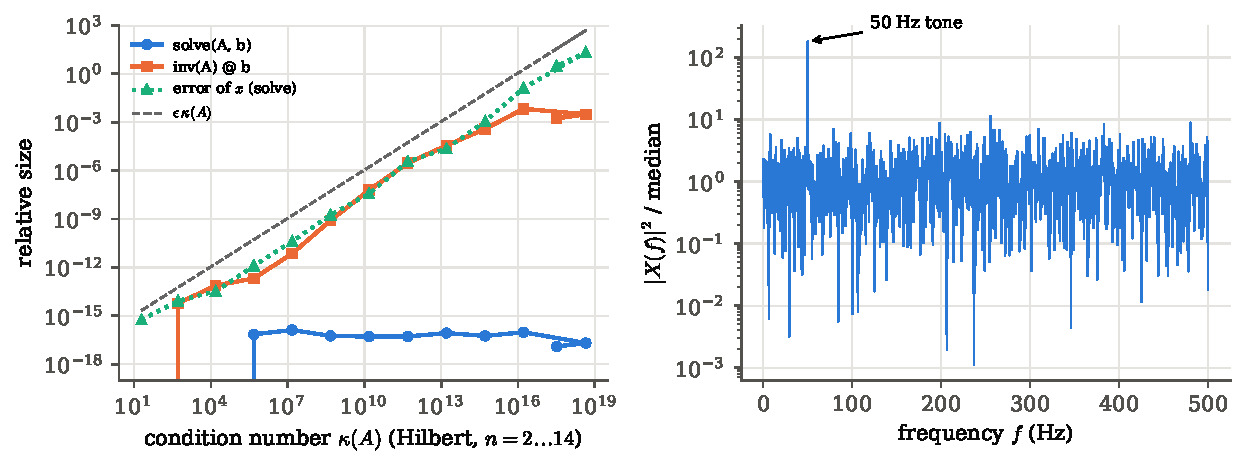
\includegraphics[width=12cm]{figures/chT0/07_numpy_tour.pdf}
\caption{Left: solving $A\bm x=\bm b$ for Hilbert matrices of growing size. With \texttt{solve} (blue) the residual stays at the rounding level for every condition number; with \texttt{inv} followed by a product (orange) it grows with the condition number. The error of $\bm x$ itself (green) follows $\epsilon\kappa$ (dashed) whatever the method. Right: the power spectrum of $2$\,s of noise containing a weak $50$\,Hz tone, normalised to its median: one Fourier coefficient carries the tone.}
\label{T0a:fig:linalg-fft}
\end{figure}

In the book, a typical FFT is two lines inside a larger recipe. The autocorrelation of a Markov chain (\cref{9b:sec:tau}) is computed with the Wiener--Khinchin theorem: the autocorrelation is the inverse transform of the power spectrum.

\pyfile[firstline=74,lastline=81,firstnumber=74]{code/ch09/lib_mcmc9c.py}{The autocorrelation of a chain through two FFTs}

Line 76 subtracts the mean. Line 78 transforms with \texttt{n=2 * n}, which pads the series with zeros to twice its length, so that the circular wrap-around of the discrete transform does not mix the end of the chain with its beginning. Line 79 multiplies the transform by its complex conjugate (the power) and transforms back; the first $n$ entries are the autocovariance at lags $0,\dots,n-1$. Line 80 divides by the value at lag $0$, so that $\rho(0)=1$. Done directly, this would cost $n^2$ operations, about $10^{10}$ for a chain of $10^5$ steps; through the FFT it takes milliseconds.
\section{SciPy: distributions, integrals, roots and minima}
\label{T0a:sec:scipy}

NumPy does arithmetic on arrays. SciPy adds the classic numerical recipes that a physicist would otherwise copy from a handbook: the densities and tail probabilities of the standard distributions, numerical integration, root finding, minimisation, special functions and interpolation. It is used in $\TzPctScipy\%$ of the scripts but makes only $\TzScipyShare\%$ of the calls, because one SciPy call does a lot of work. Six tools cover almost all of it. Each is shown answering one small physics question in \pyname{code/chT0/03_scipy_tour.py}, with an answer we can check by hand, and then in a real script.

\subsection{Probability distributions}
\label{T0a:sec:stats}

\texttt{scipy.stats} contains one object per distribution: \texttt{stats.norm}, \texttt{stats.poisson}, \texttt{stats.binom}, \texttt{stats.chi2}, \texttt{stats.t}, \texttt{stats.expon}, and about a hundred more. Every object answers the same five questions, which are the five things the earlier chapters ask of a distribution (\cref{T0a:fig:scipy}, left):
\begin{center}
\begin{tabular}{@{}lll@{}}
\toprule
method & question & formula \\
\midrule
\texttt{pdf(x)} (\texttt{pmf} if discrete) & how dense is the probability at $x$? & $p(x)$\\
\texttt{cdf(x)} & how likely is a value at most $x$? & $F(x)=\Prob(X\le x)$\\
\texttt{sf(x)} & how likely is a value above $x$? & $1-F(x)$, computed directly\\
\texttt{ppf(q)} & below which value lies a fraction $q$? & $F^{-1}(q)$\\
\texttt{rvs(size=n)} & give me $n$ random draws & \\
\bottomrule
\end{tabular}
\end{center}
Shape parameters come first (\texttt{stats.poisson.pmf(k, mu)}, \texttt{stats.chi2.sf(x, df)}), and every continuous distribution also takes \texttt{loc} and \texttt{scale}, which shift and stretch it: \texttt{stats.norm.pdf(x, loc=mu, scale=sigma)} is the Gaussian of mean $\mu$ and standard deviation $\sigma$. The logarithmic versions \texttt{logpdf}, \texttt{logpmf} and \texttt{logsf} are what likelihoods use, because a product of many small densities underflows while a sum of their logarithms does not (\cref{T0a:sec:precision}).

\pyfile[firstline=24,lastline=29,firstnumber=24]{code/chT0/03_scipy_tour.py}{One distribution object, several questions}

Line 25 asks where the Gaussian cdf reaches $0.975$: the answer, $\TzZninetyfive$, is the familiar ``$1.96\sigma$'' of a two-sided $95\%$ interval, and \texttt{cdf} of it gives back $\TzBackCdf$. Line 26 asks for the probability of a fluctuation above $5\sigma$: $\TzPfive$, the discovery threshold of particle physics. Line 27 draws $10^4$ values from $\Normal(2,0.5^2)$ using the book's generator (\texttt{random\_state=rng}); their sample mean and standard deviation are $\TzRvsMean$ and $\TzRvsStd$.

The same two functions do the work of the $p$-value-to-sigma conversion of \cref{4a:sec:p-to-z}:

\pyfile[firstline=23,lastline=25,firstnumber=23]{code/ch04/09_p_to_z.py}{Sigmas to one- and two-sided $p$-values}

\texttt{stats.norm.sf(Z)} acts on the whole array \texttt{Z} $=1,\dots,6$ at once, like any NumPy function. The reverse direction, from a $p$-value to a number of sigmas, is \texttt{stats.norm.isf(p)}, the inverse of \texttt{sf}.

\begin{pitfall}[\texttt{1 - cdf} in the tail]
For $x$ far in the upper tail, $F(x)$ is a number like $0.9999999997$, and $1-F(x)$ keeps only the few digits that differ from $1$. \texttt{sf(x)} computes the tail directly and keeps all sixteen. At $5\sigma$ the difference is still small; beyond about $8\sigma$, \texttt{1 - cdf} returns exactly $0$ while \texttt{sf} is still accurate (\cref{T0a:sec:precision}).
\end{pitfall}

\subsection{Integrals}
\label{T0a:sec:quad}

\texttt{integrate.quad(f, a, b)} integrates a function of one variable from \texttt{a} to \texttt{b} (either limit may be \texttt{np.inf}) and returns \emph{two} numbers: the value and an estimate of its absolute error. It evaluates \texttt{f} at cleverly chosen points, compares two rules of different order on each piece of the interval, and keeps subdividing the pieces where they disagree. The tour checks it against the $5\sigma$ tail of line 26:

\pyfile[firstline=31,lastline=33,firstnumber=31]{code/chT0/03_scipy_tour.py}{The $5\sigma$ tail again, by integrating the density}

\texttt{quad} returns $\TzQuadTail$ with an error estimate of $\TzQuadErr$, and the value differs from \texttt{sf(5)} by a relative $\TzQuadRel$. The comma on the left, \texttt{tail, tail\_err = \dots}, unpacks the two returned numbers. Many scripts keep only the value, writing \texttt{quad(\dots)[0]}, as the detector-smearing check of \cref{1b:sec:joint} does:

\pyfile[firstline=60,lastline=62,firstnumber=60]{code/ch01/13_detector_smearing.py}{Expected counts per histogram bin from integrals of a density}

Line 62 is a list comprehension that integrates the density over every bin, \texttt{zip(edges[:-1], edges[1:])} pairing each left edge with the next one. \Cref{T0a:sec:trust-boxes} shows how the error estimate can be wrong, and what to do about it.

\subsection{Roots}
\label{T0a:sec:roots}

Many statistical answers are the solution of one equation in one unknown: the parameter value where $\ln\Like$ has dropped by $\tfrac12$, the mean $\mu$ at which observing so few events would have probability $5\%$, the Lagrange multiplier of a maximum-entropy problem. \texttt{optimize.brentq(f, a, b)} finds a zero of \texttt{f} between \texttt{a} and \texttt{b}. It requires a \newterm{bracket}: \texttt{f(a)} and \texttt{f(b)} must have opposite signs, so that a continuous \texttt{f} must cross zero in between. It then shrinks the bracket, combining halving (always safe) with interpolation steps (fast when $f$ is smooth), until the zero is pinned to about $10^{-12}$ (\cref{T0a:fig:brentq}).

\begin{figure}[htbp]
\centering
\begin{tikzpicture}
\begin{axis}[width=8.5cm,height=5.0cm,xmin=0,xmax=2.05,ymin=-2.5,ymax=2.3,
  axis lines=middle,xlabel={$x$},ylabel={$f(x)=x^2-2$},
  xlabel style={anchor=north west},ylabel style={anchor=south},
  xtick={0,0.5,1,1.5,2},ytick={-2,-1,0,1,2},tick label style={font=\scriptsize},
  label style={font=\small}]
  \addplot[domain=0:2,samples=100,thick,formblue] {x^2-2};
  \addplot[only marks,mark=*,mark size=1.6pt,bdryred] coordinates {(0,-2) (2,2)};
  \addplot[only marks,mark=*,mark size=1.6pt,fibreorange] coordinates {(1,-1) (1.5,0.25)};
  \addplot[only marks,mark=*,mark size=2pt,tangentgreen] coordinates {(1.41421356,0)};
  \node[font=\scriptsize,anchor=west,bdryred] at (axis cs:0.08,-2.3) {$f(0)<0$};
  \node[font=\scriptsize,anchor=east,bdryred] at (axis cs:1.95,2.0) {$f(2)>0$};
  \node[font=\scriptsize,anchor=north west,fibreorange] at (axis cs:1.03,-1.08) {midpoint $1$};
  \node[font=\scriptsize,anchor=south east,fibreorange] at (axis cs:1.5,0.6) {midpoint $1.5$};
  \node[font=\scriptsize,anchor=south east,tangentgreen] at (axis cs:1.40,0.05) {$\sqrt2$};
\end{axis}
\end{tikzpicture}
\caption{A bracket and its shrinking. $f(0)=-2<0$ and $f(2)=2>0$ (red points), so a zero lies in $[0,2]$. The midpoint $1$ has $f<0$, so the zero is in $[1,2]$; the next midpoint $1.5$ has $f>0$, so it is in $[1,1.5]$ (orange points). \texttt{brentq} mixes such halvings with faster interpolation steps and stops at $\sqrt2$ (green) to twelve digits. On $[0,1]$ there is no sign change and \texttt{brentq} refuses to start.}
\label{T0a:fig:brentq}
\end{figure}

The tour computes the $95\%$ upper limit on a Poisson mean after observing $n$ events: the $\mu$ at which $\Prob(N\le n\given\mu)=0.05$.

\pyfile[firstline=35,lastline=39,firstnumber=35]{code/chT0/03_scipy_tour.py}{An upper limit as the root of an equation}

For $n=0$ the equation is $e^{-\mu}=0.05$, whose exact root is $\ln20=\TzUpperZeroExact$; \texttt{brentq} gives $\TzUpperZero$. For $n=3$ it gives $\TzUpperThree$ (\cref{T0a:fig:scipy}, right). The likelihood interval of the decay-time example (\cref{T0a:sec:functions}, lines 39--40 there) is the same pattern, with two brackets, one on each side of the maximum.

\subsection{Minima}
\label{T0a:sec:minimize}

{\sloppy Maximum likelihood means finding the parameters that make $-\ln\Like$ smallest. \texttt{optimize.minimize(f, x0)} starts at the guess \texttt{x0} and walks downhill. It returns a result object whose most useful entries are \texttt{res.x} (the minimising parameters), \texttt{res.fun} (the value there), \texttt{res.success} (whether the method believes it converged) and \texttt{res.nit} (how many iterations it took). The \texttt{method} keyword chooses the walk: \texttt{"Nelder-Mead"} needs only function values and is robust; \texttt{"BFGS"} and \texttt{"L-BFGS-B"} use gradients (estimated numerically if not given) and are faster on smooth problems; \texttt{"L-BFGS-B"} also accepts \texttt{bounds}. Extra fixed inputs, such as the data, are handed over with \texttt{args=(\dots,)}.\par}

\pyfile[firstline=41,lastline=48,firstnumber=41]{code/chT0/03_scipy_tour.py}{Maximum likelihood for Gaussian data by minimisation}

Two habits are visible here. The width is fitted as $\ln\sigma$ (line 43), so that any real number is an allowed value and the minimiser cannot wander to a negative $\sigma$. And the result is checked against an answer known in closed form: for Gaussian data the maximum-likelihood estimates are the sample mean and the divide-by-$n$ standard deviation. The minimiser finds $\hat\mu=\TzMinMu$ and $\hat\sigma=\TzMinSig$ in $\TzMinIters$ iterations; the closed forms give $\TzMeanCheck$ and $\TzStdCheck$.

The Poisson-binned fit of \cref{3b:sec:poisson-python} wraps \texttt{minimize} in a small function, so that three different goodness-of-fit functions can be minimised with the same call:

\pyfile[firstline=57,lastline=61,firstnumber=57]{code/ch03/12_poisson_bins.py}{A minimiser wrapped in a function, with tightened tolerances}

The function to minimise, \texttt{fun}, is itself an argument (functions can be passed around like numbers). \texttt{options=dict(xatol=\dots, fatol=\dots, maxiter=\dots)} tightens the stopping rules, because the default tolerances of Nelder--Mead are loose for a study that compares estimators to many digits. \Cref{T0a:sec:trust-boxes} shows what happens when a minimiser stops too early, and how \texttt{res.success} reports it.

\subsection{Special functions and interpolation}
\label{T0a:sec:special}

\texttt{scipy.special} contains the functions of mathematical physics: $\Gamma$ and its logarithm \texttt{gammaln}, the beta function, binomial coefficients \texttt{comb}, error functions, Bessel functions, the Voigt profile. The one the book uses most is \texttt{gammaln}, because likelihoods of counts contain factorials, and factorials overflow: $200!\approx10^{375}$ is far beyond the largest double, about $1.8\times10^{308}$. Its logarithm is a modest number:

\pyfile[firstline=50,lastline=57,firstnumber=50]{code/chT0/03_scipy_tour.py}{$\ln 200!$ is fine; $200!$ as a float is not}

$\ln200!=\ln\Gamma(201)=\TzLnFact$, and Python's own \texttt{math.lgamma} agrees ($\TzLnFactCheck$). Converting $200!$ itself to a float overflows (\texttt{OverflowError}: \TzFactOverflow); the \texttt{try}/\texttt{except} block of lines 52--56 catches that error and records it instead of stopping (\cref{T0a:sec:rare}). The de Moivre--Laplace check of \cref{2b:sec:dml-python} uses \texttt{special.gammaln(n\_st + 1)} for exactly this reason.

\newterm{Interpolation} estimates a function between tabulated points. \texttt{np.interp(x, xt, yt)} joins the table $(x_t,y_t)$ by straight lines; \texttt{interpolate.CubicSpline(xt, yt)} by smooth cubic pieces whose first and second derivatives are continuous. For a coarse table of six values of $\sin x$ on $[0,\pi]$ the tour finds a largest error of $\TzInterpLinErr$ for straight lines and $\TzInterpSplErr$ for the spline (lines 59--66). Straight lines are the right choice when the table is fine and the curve may have kinks; a spline when the table is coarse and the curve is smooth. \texttt{np.interp} is the one the book calls most often, typically to read a tabulated CAMB spectrum or a transfer function at new multipoles.

\begin{figure}[htbp]
\centering
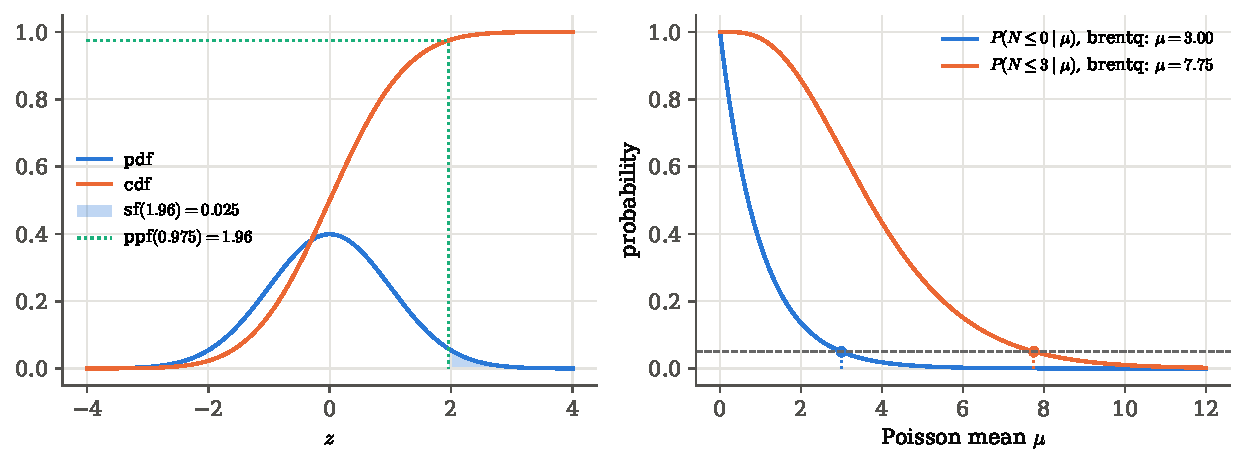
\includegraphics[width=12cm]{figures/chT0/03_scipy_tour.pdf}
\caption{Left: the standard Gaussian's density (pdf) and cumulative distribution (cdf). The shaded tail above $1.96$ is \texttt{sf(1.96)} $=0.025$, and the dotted path from $0.975$ on the cdf down to the axis is \texttt{ppf(0.975)} $=1.96$. Right: the probability of observing at most $n$ events as a function of the Poisson mean, for $n=0$ and $3$; \texttt{brentq} finds where each curve crosses $0.05$ (dashed), the $95\%$ upper limits.}
\label{T0a:fig:scipy}
\end{figure}
\section{Matplotlib, files and folders}
\label{T0a:sec:plots}

Every figure drawn from data in the book is made by a dozen Matplotlib calls, and every expensive result is kept on disk by two NumPy calls. Both are learned once.

\subsection{A figure is a canvas holding axes}
\label{T0a:sec:matplotlib}

Matplotlib thinks of a picture in two layers (\cref{T0a:fig:mpl}). The \newterm{figure} is the whole canvas, the thing saved to a PDF file. On it sit one or more \newterm{axes}: rectangular panels, each with its own coordinate system, ticks, labels and legend. Everything that is drawn is drawn \emph{on an axes}. The book always creates both at once,
\begin{center}
\texttt{fig, ax = plt.subplots()} \qquad or \qquad \texttt{fig, axes = plt.subplots(2, 3)}
\end{center}
which returns the figure and one axes, or the figure and a $2\times3$ array of axes, \texttt{axes[row, column]}. Everything else is a method of \texttt{ax}:
\begin{center}
\small
\begin{tabular}{@{}ll@{}}
\toprule
call & draws \\
\midrule
\texttt{ax.plot(x, y)}, \texttt{ax.plot(x, y, "o")} & a line through the points, or markers only\\
\texttt{ax.loglog}, \texttt{ax.semilogx}, \texttt{ax.semilogy} & the same with logarithmic axes\\
\texttt{ax.hist(data, bins=40, density=True)} & a histogram, normalised to a density\\
\texttt{ax.errorbar(x, y, yerr=s, fmt="o")} & points with error bars\\
\texttt{ax.fill\_between(x, lo, hi, alpha=0.3)} & a shaded band\\
\texttt{ax.imshow(image, origin="lower")} & a two-dimensional array as an image\\
\texttt{ax.axhline(y)}, \texttt{ax.axvline(x)} & a horizontal or vertical reference line\\
\texttt{ax.set\_xlabel}, \texttt{set\_ylabel}, \texttt{set\_title}, \texttt{set\_xlim} & labels and ranges\\
\texttt{ax.legend()} & a key built from the \texttt{label=\dots} of each curve\\
\bottomrule
\end{tabular}
\end{center}
Finally \texttt{fig.tight\_layout()} packs the panels so that labels do not overlap, and the book's \texttt{savefig(fig, "chNN", "name")} writes the PDF into \texttt{figures/chNN/} (\cref{0a:sec:code}). Colours come from the house palette set by \texttt{setup()}, and every analytic curve is drawn by \texttt{theory\_line(ax, x, y)} as a black dashed line on top of the simulation it is compared with.

\begin{figure}[htbp]
\centering
\begin{tikzpicture}[x=1cm,y=1cm]
  \draw[thick,softgray,fill=white] (0,0) rectangle (10.2,4.6);
  \node[font=\footnotesize\ttfamily,softgray,anchor=north west] at (0.05,4.6) {fig};
  \foreach \xo/\lab in {0.9/{axes[0]},5.9/{axes[1]}} {
    \begin{scope}[shift={(\xo,0.8)}]
      \draw[accent,fill=ideabg] (0,0) rectangle (3.6,3.0);
      \node[font=\footnotesize\ttfamily,accent,anchor=south west] at (0,3.0) {\lab};
    \end{scope}
  }
  \begin{scope}[shift={(0.9,0.8)}]
    \draw[formblue,thick,domain=0.1:3.5,samples=60] plot (\x,{1.5+1.1*exp(-\x/1.5)*cos(deg(2.2*\x))});
    \foreach \t in {0.3,0.7,...,3.3} { \fill[fibreorange] (\t,{1.5+1.1*exp(-\t/1.5)*cos(deg(2.2*\t))+0.12*sin(deg(7*\t))}) circle (1.3pt); }
    \node[font=\scriptsize,anchor=north] at (1.8,-0.05) {\texttt{ax.set\_xlabel("time")}};
    \node[font=\scriptsize,rotate=90,anchor=south] at (-0.05,1.5) {\texttt{set\_ylabel}};
    \draw[softgray] (2.25,2.35) rectangle (3.5,2.9);
    \node[font=\scriptsize,anchor=west] at (2.28,2.62) {\texttt{legend}};
  \end{scope}
  \begin{scope}[shift={(5.9,0.8)}]
    \foreach \i/\h in {0/0.25,1/0.6,2/1.25,3/2.0,4/2.4,5/2.1,6/1.3,7/0.65,8/0.3} {
      \fill[formblue!45] ({0.2+0.35*\i},0) rectangle ({0.5+0.35*\i},\h);
    }
    \draw[black,thick,dashed,domain=0.1:3.4,samples=60] plot (\x,{2.45*exp(-((\x-1.75)^2)/(2*0.62^2))});
    \node[font=\scriptsize,anchor=north] at (1.8,-0.05) {\texttt{ax.hist} + \texttt{theory\_line}};
  \end{scope}
\end{tikzpicture}
\caption{The two layers of a Matplotlib picture. The figure (\texttt{fig}) is the canvas that is saved; each axes is one panel with its own coordinates, and everything is drawn by a method of an axes. \texttt{plt.subplots(1, 2)} creates this layout and returns the figure and the array of the two axes.}
\label{T0a:fig:mpl}
\end{figure}

The gallery script \pyname{code/chT0/04_plot_gallery.py} draws one panel of each common kind from simulated data (\cref{T0a:fig:gallery}). A real figure of the book is the same calls in a slightly longer sequence. Here is the log-likelihood plot of the decay-time example (\cref{3b:sec:curv-python}):

\pyfile[firstline=42,lastline=53,firstnumber=42]{code/ch03/09_mle_decay.py}{A complete figure: curve, theory, reference lines, labels, legend, save}

Line 42 makes one axes of $5.2\times3.2$ inches. Line 44 plots $\ln\Like(\tau)-\ln\Like_{\max}$ on a grid of $400$ values of $\tau$, with a \LaTeX{} label for the legend (the \texttt{r} before the string keeps the backslashes, \cref{T0a:sec:strings}). Line 45 overlays the parabola that has the same curvature at the maximum. Lines 46--48 add a dotted horizontal line at $-\tfrac12$ and vertical lines at the two roots found by \texttt{brentq}. Lines 49--51 set the range, the axis labels and the legend; line 53 saves.

\begin{figure}[htbp]
\centering
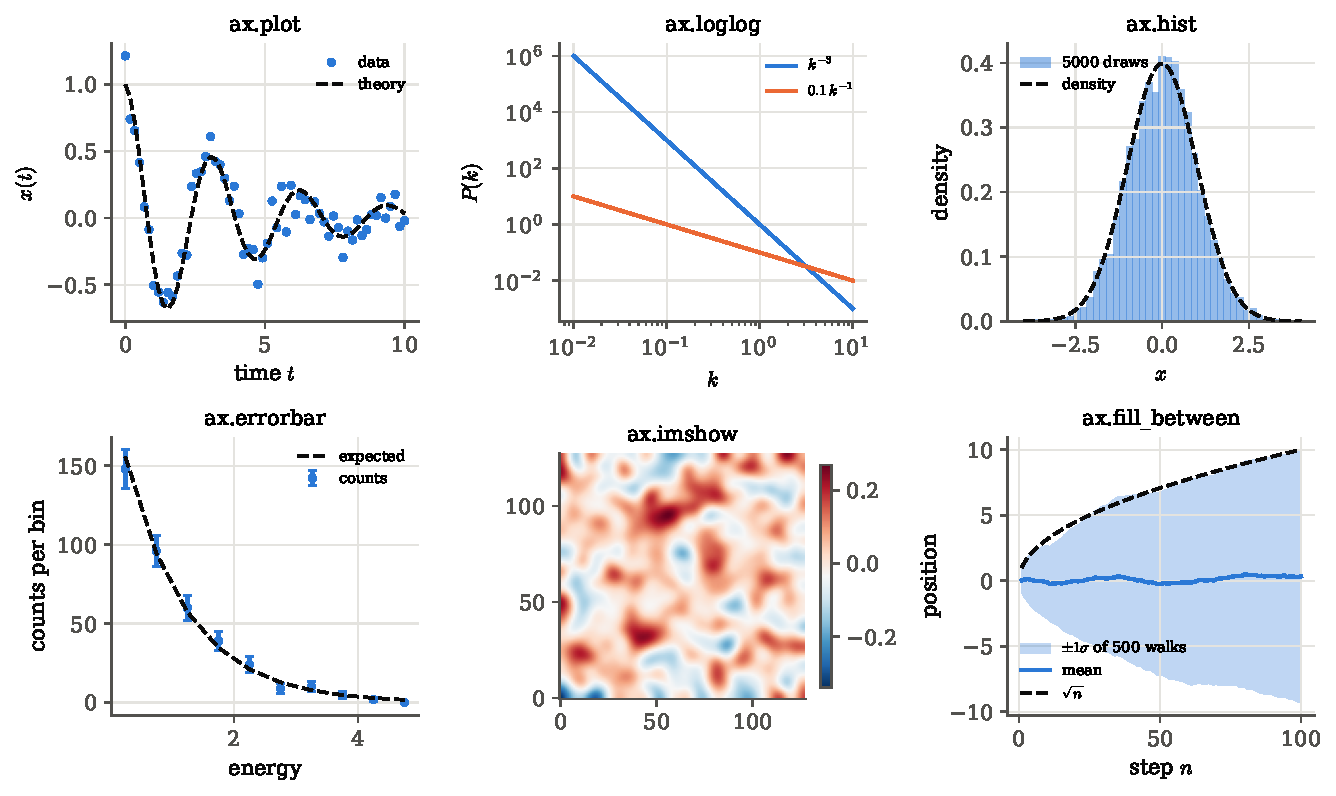
\includegraphics[width=\linewidth]{figures/chT0/04_plot_gallery.pdf}
\caption{Six kinds of panel and the call that draws each, from simulated data: noisy samples of a damped oscillation with the curve they scatter around (\texttt{plot}), two power laws as straight lines on logarithmic axes (\texttt{loglog}), $5000$ Gaussian draws against their density (\texttt{hist}), Poisson counts with $\sqrt n$ error bars (\texttt{errorbar}), a smoothed random field (\texttt{imshow}), and the $\pm1\sigma$ band of $500$ random walks around their mean, against $\sqrt n$ (\texttt{fill\_between}).}
\label{T0a:fig:gallery}
\end{figure}

\paragraph{Example: why a histogram needs \texttt{density=True}.} A histogram of $5000$ draws in bins of width $\Delta x$ has heights $n_j$ that add up to $5000$. A density $p(x)$ integrates to $1$. To compare them, the heights must be divided by the number of draws and by the bin width:
\begin{align*}
  \hat p_j
  &\eqby{1}\frac{n_j}{N\,\Delta x},
  &
  \sum_j\hat p_j\,\Delta x
  &\eqby{2}\frac{1}{N}\sum_j n_j
   \eqby{3}1 .
\end{align*}
\begin{explain}
  \item The fraction of draws in bin $j$, $n_j/N$, estimates $\int_{\text{bin}}p\,\dd x\approx p(x_j)\,\Delta x$; divide by $\Delta x$.
  \item Multiply each height by its bin width and add.
  \item Every draw falls in some bin (if the bins cover the data), so the counts add up to $N$.
\end{explain}
\texttt{ax.hist(x, bins=40, density=True)} does exactly this division, which is why the histogram and the black dashed density in the third panel of \cref{T0a:fig:gallery} lie on top of each other. Without \texttt{density=True} the bars would be $N\,\Delta x\approx5000\times0.2=1000$ times taller than the curve (for $40$ bins over a range of about $8$, $\Delta x\approx0.2$).

\begin{pitfall}[\texttt{plt} versus \texttt{ax}]
Many examples on the internet draw with \texttt{plt.plot(\dots)}, which draws on ``the current axes'' that Matplotlib keeps in the background. With several panels, ``current'' is easily not the panel intended. The book always draws with \texttt{ax.plot(\dots)} on an axes it holds by name, and calls \texttt{plt} only to create the figure.
\end{pitfall}

\subsection{Files, folders and caches}
\label{T0a:sec:files}

Some results cost minutes or hours: a thousand simulated CMB skies, a long Markov chain, a hundred calls of a Boltzmann code. They are computed once and kept in the folder \texttt{data/}, in NumPy's own file format. Two calls do it. \texttt{np.savez(path, name1=array1, name2=array2)} writes several arrays into one \texttt{.npz} file, each under a name. \texttt{z = np.load(path)} opens it, and \texttt{z["name1"]} gives back the first array, bit for bit.

Paths are handled by Python's \texttt{pathlib}. A \texttt{Path} is a file or folder name that knows its structure: \texttt{NOTES / "data" / "ch08"} joins names with the operator \texttt{/}, whatever the operating system's separator; \texttt{path.exists()} asks whether the file is there; \texttt{path.mkdir(parents=True, exist\_ok=True)} creates a folder (and any missing folders above it) unless it already exists; \texttt{path.parents[1]} is two levels up (\cref{T0a:sec:anatomy}).

The two combine into the \newterm{cache} pattern: if the file exists, load it; otherwise compute, save, and return. The Monte Carlo library of \cref{8a:sec:pipeline} writes it once, as a function that takes the computation itself as an argument:

\pyfile[firstline=252,lastline=262,firstnumber=252]{code/ch08/lib_cmbsim.py}{Compute once, then load: a cache in eleven lines}

\texttt{make} is a function that returns a dictionary of arrays (line 252 receives it without calling it). Line 254 makes sure \texttt{data/ch08} exists. If the file is already there and recomputing was not forced (line 256), lines 257--258 load it and turn it back into a dictionary with a comprehension over \texttt{z.files}, the list of the names stored in it. Otherwise line 259 calls \texttt{make()}, line 260 saves every entry of the dictionary with \texttt{**d} (which hands each key--value pair to \texttt{np.savez} as a keyword argument), and line 262 returns the result. A thousand skies are simulated the first time; every later run of every script that needs them reads them in a fraction of a second (\cref{T0a:fig:cache}).

\begin{figure}[htbp]
\centering
\begin{tikzpicture}[
  box/.style={draw=accent,rounded corners=2pt,fill=ideabg,align=center,font=\footnotesize,
              text width=2.7cm,minimum height=0.9cm,inner sep=3pt},
  q/.style={draw=accent,diamond,aspect=2.2,fill=white,font=\footnotesize,align=center,inner sep=1pt},
  arr/.style={->,thick,accent}]
  \node[box] (call) at (0,0) {\texttt{cached("mc", make)}};
  \node[q] (ex) at (3.9,0) {file\\ exists?};
  \node[box,fill=takebg,draw=tangentgreen] (load) at (8.0,0.85) {\texttt{np.load}: seconds};
  \node[box,fill=warnbg,draw=bdryred] (make) at (8.0,-0.85) {\texttt{make()}: minutes or hours};
  \node[box] (save) at (11.4,-0.85) {\texttt{np.savez}};
  \draw[arr] (call) -- (ex);
  \draw[arr] (ex.north) |- node[pos=0.75,above,font=\scriptsize] {yes} (load.west);
  \draw[arr] (ex.south) |- node[pos=0.75,below,font=\scriptsize] {no} (make.west);
  \draw[arr] (make) -- (save);
\end{tikzpicture}
\caption{The cache pattern of \texttt{lib\_cmbsim.cached}. The expensive branch (red) runs once and leaves a file behind; every later call takes the cheap branch (green). Deleting the file, or passing \texttt{force=True}, forces a fresh computation.}
\label{T0a:fig:cache}
\end{figure}

The fiducial CMB spectra shared by the whole book are cached the same way, in \pyname{code/camb_fiducial.py}:

\pyfile[firstline=25,lastline=37,firstnumber=25]{code/camb_fiducial.py}{Load the cached CAMB spectra, computing them on first use}

\texttt{load\_fiducial()} computes and saves the spectra only if \texttt{data/camb\_fiducial.npz} is missing (lines 26--27), and otherwise loads them (line 28) and returns the multipoles and the requested spectrum (line 29). Line 36 shows one more use of \texttt{**}: it unpacks a dictionary built on the spot, so that the parameters of the fiducial model are stored in the same file as \texttt{param\_H0}, \texttt{param\_ombh2}, and so on, and anyone opening the file can see which model produced it.

\begin{pitfall}[A stale cache]
A cache does not know that the code which produced it has changed. If a simulation is corrected but its cache file is left in place, every script keeps reading the old, wrong results. After changing a computation that feeds a cache, delete the file (or run once with \texttt{force=True}).
\end{pitfall}
\section{Seen a few times: rare features and two black boxes}
\label{T0a:sec:rare}

The census (\cref{T0a:fig:syntax}) found a sharp drop after the core of the language: a few constructions appear in fewer than one script in ten. They can be skipped on a first reading and looked up here when met. The same holds for the two physics libraries, healpy and CAMB, which the book uses as black boxes: we need to know what goes in and what comes out, not how they work inside.

\subsection{Classes and data classes}
\label{T0a:sec:classes}

A \newterm{class} bundles data together with the functions that act on it. The book defines classes in only $\TzPctClass\%$ of its scripts, always for the same reason: a group of settings that belong together and some quantities derived from them. The clearest example is the description of a CMB experiment in the Monte Carlo library of \cref{8a:sec:beam}:

\pyfile[firstline=68,lastline=92,firstnumber=68]{code/ch08/lib_cmbsim.py}{An experiment as a data class: settings, and quantities derived from them}

Read it as a form with blanks. Line 68, \texttt{@dataclass}, is a \newterm{decorator}: a line starting with \texttt{@} that modifies the definition below it, here by writing the routine parts of the class automatically. Lines 71--75 list the settings, each with a type hint and a default value: the HEALPix resolution, the beam width, the noise level, the band limit, and whether to include the pixel window. Then \texttt{exp = Experiment(nside=128, fwhm\_arcmin=10.0)} creates one experiment with two settings changed and the rest left at their defaults, and \texttt{exp.nside} reads a setting back. Lines 77--91 define quantities computed from the settings. The decorator \texttt{@property} makes each of them look like a setting: \texttt{exp.npix} or \texttt{exp.sigma\_pix} without brackets, recomputed every time it is read, so it can never disagree with the settings. Inside the class, \texttt{self} means ``this particular experiment''. Lines 92 onwards are ordinary functions of the experiment, called as \texttt{exp.nl()}.

\subsection{Errors on purpose, and \texttt{with}}
\label{T0a:sec:try-with}

\texttt{try:} followed by \texttt{except SomeError:} runs a block and, if that particular error occurs, runs the second block instead of stopping. It appears in $\TzPctTry\%$ of the scripts, typically to record that something failed. The SciPy tour uses it to show that $200!$ cannot be a float (\cref{T0a:sec:special}), and \cref{T0a:sec:trust-linalg} uses it to detect a matrix that is not positive definite. Catching errors to hide them is never done: a script that fails should fail loudly.

\texttt{with \dots{} as name:} sets something up for the duration of an indented block and tidies it away afterwards, even if the block fails. It appears in $\TzPctWith\%$ of the scripts, in three forms: opening a file, starting a pool of worker processes (below), and \texttt{with np.errstate(divide="ignore"):}, which silences NumPy's warning about a division by zero that the code is about to repair anyway (line 54 of \pyname{lib_fields.py}, where $P(k)$ is evaluated at $k=0$ and then set to zero).

\subsection{Several cores at once}
\label{T0a:sec:pool}

A Monte Carlo study runs the same function on many independent random seeds, and those runs can go on different processor cores at the same time. Python's \texttt{multiprocessing.Pool} does this with one call: \texttt{pool.map(f, jobs)} applies \texttt{f} to every item of the list \texttt{jobs}, spreads the items over the workers, and returns the results in the original order. The topology study of \cref{12c:sec:model} is the clearest case:

\pyfile[firstline=50,lastline=69,firstnumber=50]{code/ch12/c02_mc_fnl.py}{Hundreds of independent simulations spread over four cores}

Each job (lines 64--66) is a tuple: a stream number and a list of non-Gaussianity amplitudes $\epsilon$. The function \texttt{one} (lines 50--60) makes its own generator from the stream number (line 52), draws one Gaussian field, and measures it at every $\epsilon$ in the list. Line 68 starts four workers, and line 69 runs all the jobs. Two details make this safe. Every job builds its generator from its own stream number, so the result does not depend on which worker ran which job or in what order (\cref{T0a:sec:random}); a generator shared between workers would make the results depend on the scheduling. And the function given to \texttt{pool.map} is defined at the top level of the module, because each worker process imports the script to find it.

\begin{figure}[htbp]
\centering
\begin{tikzpicture}[
  job/.style={draw=softgray,fill=codebg,font=\scriptsize\ttfamily,minimum width=1.0cm,minimum height=0.5cm,inner sep=0.5pt},
  wk/.style={draw=accent,rounded corners=2pt,fill=ideabg,font=\footnotesize,minimum width=1.9cm,minimum height=0.6cm},
  arr/.style={->,accent}]
  \foreach \i in {0,...,7} { \node[job] (j\i) at (1.1*\i,0) {(\i,\dots)}; }
  \node[font=\footnotesize,anchor=east] at (-0.7,0) {\texttt{jobs}};
  \foreach \w in {0,...,3} { \node[wk] (w\w) at (0.25+2.4*\w,-1.6) {worker \w}; }
  \foreach \i/\w in {0/0,1/1,2/2,3/3,4/0,5/1,6/2,7/3} { \draw[arr] (j\i.south) -- (w\w.north); }
  \foreach \i in {0,...,7} { \node[job,fill=takebg,draw=tangentgreen] (r\i) at (1.1*\i,-3.2) {res \i}; }
  \foreach \i/\w in {0/0,1/1,2/2,3/3,4/0,5/1,6/2,7/3} { \draw[arr,tangentgreen] (w\w.south) -- (r\i.north); }
  \node[font=\footnotesize,anchor=east] at (-0.7,-3.2) {\texttt{out}};
\end{tikzpicture}
\caption{\texttt{pool.map(one, jobs)} with four workers. Each job carries its own stream number, so it produces the same result whichever worker runs it, and the list of results comes back in the order of the jobs.}
\label{T0a:fig:pool}
\end{figure}

\subsection{Compiled loops: numba}
\label{T0a:sec:numba}

Vectorisation (\cref{T0a:sec:vectorise}) needs the elements to be independent, so that one operation can act on all of them. Some algorithms are sequential by nature: in a Metropolis sweep of the Ising model each spin's update depends on its neighbours' \emph{current} values, which earlier steps of the same sweep may have just changed. Such a loop cannot be written as one array expression. The library numba solves this by compiling a Python function into machine code the first time it is called: the decorator \texttt{@njit} on top of the function is the only change. Five files use it ($\TzPctNumba\%$). The Ising sweep of \cref{9b:sec:ising} is one:

\pyfile[firstline=19,lastline=35,firstnumber=19]{code/ch09/20_ising.py}{A sequential Metropolis sweep, compiled by numba}

Apart from line 19 this is plain Python with two nested loops: visit every site, sum its four neighbours with periodic wrap-around (the \texttt{\% L} on line 28), compute the energy change, and accept the flip with the Metropolis probability. Uncompiled, the $L^2$ inner steps would run at Python's speed of a few hundred nanoseconds each; compiled, at a few nanoseconds. A compiled function accepts only NumPy arrays and plain numbers, which is why the random numbers \texttt{u} are drawn outside, by the book's generator, and passed in.

\subsection{healpy and CAMB as black boxes}
\label{T0a:sec:blackbox}

Two libraries do physics that the book does not reimplement. \newterm{healpy} handles maps on the sphere in the HEALPix pixelisation \cite{Gorski2005}: $12N_{\rm side}^2$ pixels of equal area, and the spherical-harmonic transforms between a map and its coefficients $\alm$. \newterm{CAMB} \cite{CAMB2000} solves the linearised Boltzmann equations of a cosmological model and returns its predicted spectra. Neither needs to be understood inside. Each can be used as a box with known inputs and outputs (\cref{T0a:fig:blackbox}), and checked from outside on a case with a known answer.

\begin{figure}[htbp]
\centering
\begin{tikzpicture}[
  bb/.style={draw=black!70,thick,fill=black!8,rounded corners=2pt,minimum width=2.6cm,minimum height=1.1cm,font=\small\bfseries,align=center},
  io/.style={font=\footnotesize,align=left},
  arr/.style={->,thick,accent}]
  \node[bb] (camb) at (0,0) {CAMB};
  \node[io,anchor=east] (ci) at (-2.0,0) {$H_0,\ \omega_b,\ \omega_c,\ \tau,\ A_s,\ n_s$\\ \texttt{lmax}};
  \node[io,anchor=west] (co) at (2.0,0) {$\Cell^{TT},\ \Cell^{EE},\ \Cell^{BB},\ \Cell^{TE}$\\ $\ell=0,\dots,\ell_{\max}$, in $\mu$K$^2$};
  \draw[arr] (ci.east) -- (camb.west);
  \draw[arr] (camb.east) -- (co.west);
  \node[bb] (hp1) at (0,-2.0) {\texttt{hp.alm2map}};
  \node[io,anchor=east] (hi) at (-2.0,-2.0) {$\alm$ ($\ell\le\ell_{\max}$), $N_{\rm side}$};
  \node[io,anchor=west] (ho) at (2.0,-2.0) {a map: $12N_{\rm side}^2$ pixel values};
  \draw[arr] (hi.east) -- (hp1.west);
  \draw[arr] (hp1.east) -- (ho.west);
  \node[bb] (hp2) at (0,-3.6) {\texttt{hp.anafast}};
  \node[io,anchor=east] (ai) at (-2.0,-3.6) {a map, \texttt{lmax}};
  \node[io,anchor=west] (ao) at (2.0,-3.6) {$\Chat=\frac1{2\ell+1}\sum_m|\alm|^2$};
  \draw[arr] (ai.east) -- (hp2.west);
  \draw[arr] (hp2.east) -- (ao.west);
\end{tikzpicture}
\caption{Three black boxes and what crosses their walls. CAMB turns six cosmological parameters into the predicted CMB spectra. healpy's \texttt{alm2map} turns harmonic coefficients into a pixelised map, and \texttt{anafast} turns a map back into the estimated power spectrum. A round trip through the last two must return the spectrum that went in, which is how the book checks them.}
\label{T0a:fig:blackbox}
\end{figure}

The whole CAMB interface the book uses is three calls in \pyname{code/camb_fiducial.py}:

\pyfile[firstline=16,lastline=22,firstnumber=16]{code/camb_fiducial.py}{Six parameters in, four spectra out}

Line 18 collects the parameters into one object (the \texttt{**params} unpacks the dictionary \texttt{FIDUCIAL} of line 13 into keyword arguments such as \texttt{H0=67.36}); \texttt{lmax} is set $200$ above the multipoles wanted, because the lensing calculation needs a margin. Line 19 runs the Boltzmann code, which takes several seconds. Line 20 asks for the spectra in $\mu$K$^2$ as raw $\Cell$ (not $D_\ell$), and line 21 keeps the total (lensed) spectra, an array with one row per $\ell$ and four columns $TT$, $EE$, $BB$, $TE$. Because this costs seconds per call, the result is cached (\cref{T0a:sec:files}) and CAMB is called again only by the few scripts that vary the parameters (\cref{T1a:sec:cl-response}, \cref{10a:sec:numderiv-camb}).

healpy calls look like this round trip, from \cref{7b:sec:camb}:

\pyfile[firstline=61,lastline=67,firstnumber=61]{code/ch07/24_camb_healpix.py}{From $\alm$ to a map and back: healpy as two black boxes}

Line 63 draws the coefficients with the book's own generator (\texttt{lh.synalm}, written from scratch in \cref{7b:sec:alm}). Line 64 is \texttt{hp.alm2map}: coefficients in, map of $N_{\rm side}=256$ out. Line 66 is \texttt{hp.anafast}: map in, $\Chat$ out; \texttt{iter} sets how many refinement passes it makes on the transform. Line 67 compares the result with the spectrum of the input coefficients. The few other healpy calls in the book are of the same kind: \texttt{hp.nside2npix} (pixels from resolution), \texttt{hp.map2alm} (map to coefficients), \texttt{hp.smoothing} (convolve with a beam), \texttt{hp.pixwin} (the pixel window), \texttt{hp.mollview} (draw the sphere on a page). Each is a documented box, and the book checks each once against a case with a known answer before relying on it.
\providecommand{\TzoutPart}[2]{\lstinputlisting[style=py,language={},numbers=none,
  backgroundcolor=\color{white},frame=leftline,framexleftmargin=0.6em,xleftmargin=1.2em,
  basicstyle=\ttfamily\footnotesize\color{black!75},#1]{#2}}

\section{Seven traps that catch everyone once}
\label{T0a:sec:pitfalls}

A program does exactly what it says, which is not always what its author meant. Most mistakes stop the script with an error message, and those are the friendly ones: Python names the line, and the fix is usually obvious. The dangerous mistakes are the ones that run to the end and print a plausible number. Take the smallest example. A script estimates the variance of each of $M$ simulated experiments, stored as the rows of an $M\times N$ array \texttt{x}, by subtracting each row's mean. If it writes \texttt{x - x.mean(axis=1)}, the means form an array of shape \texttt{(M,)}, and NumPy lines that shape up against the \emph{columns} of \texttt{x}, not its rows (\cref{T0a:sec:broadcasting}). When $M\neq N$ the shapes do not fit and the script stops; when by bad luck $M=N$, it subtracts the mean of experiment $j$ from reading $j$ of every experiment, runs to the end, and prints a variance that is simply wrong. The good version, \texttt{x - x.mean(axis=1, keepdims=True)}, keeps the means as a column of shape \texttt{(M, 1)} and is correct for every $M$ and $N$; its price is eleven characters. The lesson: the traps worth knowing are the silent ones.

There are seven of them, and each is a fact about how Python or NumPy stores numbers. The script \pyname{code/chT0/05_pitfalls.py} runs each one in two or three lines and prints what happens, and the book's own scripts show how each is avoided.

\subsection{Comparing real numbers}
\label{T0a:sec:pit-float}

A computer stores a real number in binary with a fixed number of digits, so most decimal fractions are stored only approximately. $0.1$ in binary is $0.000110011001100\ldots$, repeating for ever, and it is cut off after $53$ binary digits. The first lines of the script show the consequence:

\TzoutPart{firstline=1,lastline=4}{results/chT0/05_pitfalls_out.txt}

The stored $0.1+0.2$ and the stored $0.3$ differ by $\TzFloatGap$, so the test \texttt{==} says they are different. Nothing is broken: each number is correct to about sixteen significant digits, and they disagree in the seventeenth. The consequence is a rule. Real numbers computed in two different ways are compared with a tolerance, never with \texttt{==}. \texttt{np.isclose(a, b)} asks whether $\abs{a-b}\le 10^{-8}+10^{-5}\abs b$ (both tolerances can be changed with \texttt{atol=} and \texttt{rtol=}), and \texttt{np.allclose} asks the same of every element of two arrays.

The book's scripts compare in exactly this way when they check one method against another. The exact binomial confidence interval of \cref{4b:sec:ci-intentions} is found twice, once by solving two equations with \texttt{brentq} and once from a closed formula that uses the beta distribution:

\pyfile[firstline=40,lastline=45,firstnumber=40]{code/ch04/11_test_inversion.py}{Two routes to the same interval, compared with a tolerance}

Line 45 is the comparison: the two lower ends must agree to within $10^{-6}$, and so must the two upper ends. The tolerance is set by the less accurate of the two routes, here the root finder, whose default stopping rule pins the root to about $10^{-12}$; $10^{-6}$ leaves a wide margin while still catching any real mistake, which would show up in the second or third digit. How large a tolerance must be in general, and why, is the subject of \cref{T0a:sec:trust-float}.

\subsection{Whole numbers and real numbers}
\label{T0a:sec:pit-int}

Python and NumPy keep two kinds of number apart: integers (\texttt{int}, whole numbers, exact) and floating-point numbers (\texttt{float}, real numbers, approximate). Two consequences surprise newcomers:

\TzoutPart{firstline=5,lastline=7}{results/chT0/05_pitfalls_out.txt}

The first line is the dangerous one. \texttt{np.array([1, 2, 3])} is made from integers, so its \texttt{dtype} is \texttt{int64}, and an integer array can only hold integers: writing $0.7$ into it silently stores $0$, the integer part. The second line is the reassuring one: in Python~3, \texttt{/} always divides as real numbers, \texttt{7 / 2} is $3.5$, and only the explicit floor division \texttt{//} throws the fraction away.

Integer arrays arise naturally in the book, because counts are integers: \texttt{rng.poisson} and \texttt{rng.integers} return them, and so does \texttt{np.histogram} for its counts. The iterative unfolding of \cref{6b:sec:unf-bayes} works on simulated Poisson counts, and converts them to real numbers the moment they are drawn:

\pyfile[firstline=172,lastline=183,firstnumber=172]{code/ch06/30_unfolding.py}{Counts converted to real numbers before any arithmetic, and a default of \texttt{None}}

Line 183 draws $1000$ toy data sets of Poisson counts and immediately applies \texttt{.astype(float)}, which returns a copy of the array with \texttt{dtype} \texttt{float64}. The update of line 178 then divides these counts by the predicted ones and multiplies by efficiencies; with real numbers there is no risk that an intermediate result is cut to an integer anywhere along the way. (Lines 172 and 174 show another habit, the default value \texttt{None}, which \cref{T0a:sec:pit-default} explains.) The rule: when an array will hold real numbers, make it a float array from the start, with \texttt{np.zeros(n)} (which is float by default), \texttt{np.array(\dots, float)} or \texttt{.astype(float)}.

\subsection{Views and copies}
\label{T0a:sec:pit-view}

A slice of a NumPy array is not a new array. It is a \newterm{view} \unpack{a second name for part of the same block of memory}: \texttt{y = x[1:3]} makes \texttt{y} a window onto elements $1$ and $2$ of \texttt{x}, and writing through the window changes \texttt{x} (\cref{T0a:fig:view}). NumPy does this on purpose, because slicing a large array would otherwise copy it every time. The script shows both behaviours:

\TzoutPart{firstline=8,lastline=10}{results/chT0/05_pitfalls_out.txt}

With the view, the two nines appear inside \texttt{x}; with \texttt{.copy()}, \texttt{y} is an independent array and \texttt{x} stays zero. The same is true of plain assignment: \texttt{y = x} gives the same array a second name and copies nothing. Python lists behave the same way for assignment, though their slices \emph{are} copies.

\begin{figure}[htbp]
\centering
\begin{tikzpicture}[
  cell/.style={draw=black!60,minimum width=0.8cm,minimum height=0.6cm,font=\footnotesize\ttfamily},
  nm/.style={font=\small\ttfamily},
  arr/.style={->,thick,accent}]
  \node[font=\small,anchor=west] at (-0.4,1.35) {\texttt{y = x[1:3]}: a view};
  \foreach \i/\v in {0/0.,1/9.,2/9.,3/0.,4/0.} {
    \node[cell,fill=white] (a\i) at (0.8*\i,0) {\v};
    \node[font=\tiny,black!55] at (0.8*\i,-0.48) {\i};
  }
  \draw[thick,fibreorange,rounded corners=1pt] ($(a1.north west)+(-0.04,0.05)$) rectangle ($(a2.south east)+(0.04,-0.05)$);
  \node[nm,anchor=east] (x1) at (-0.75,0) {x};
  \draw[arr] (x1.east) -- (a0.west);
  \node[nm,fibreorange] (y1) at (1.2,0.95) {y};
  \draw[arr,fibreorange] (y1.south) -- ($(a1.north east)+(0,0.06)$);
  \begin{scope}[xshift=5.6cm]
  \node[font=\small,anchor=west] at (-0.4,1.35) {\texttt{y = x[1:3].copy()}};
  \foreach \i/\v in {0/0.,1/0.,2/0.,3/0.,4/0.} {
    \node[cell,fill=white] (b\i) at (0.8*\i,0) {\v};
    \node[font=\tiny,black!55] at (0.8*\i,-0.48) {\i};
  }
  \node[nm,anchor=east] (x2) at (-0.75,0) {x};
  \draw[arr] (x2.east) -- (b0.west);
  \node[cell,fill=takebg] (c0) at (1.2,-1.35) {9.};
  \node[cell,fill=takebg] (c1) at (2.0,-1.35) {9.};
  \node[nm,anchor=east,tangentgreen!60!black] (y2) at (0.25,-1.35) {y};
  \draw[arr,tangentgreen!60!black] (y2.east) -- (c0.west);
  \end{scope}
\end{tikzpicture}
\caption{Two names for one block of memory, or two blocks. Left: the slice \texttt{y} is a window (orange) onto elements $1$ and $2$ of \texttt{x}, so \texttt{y[:] = 9} writes into \texttt{x}. Right: \texttt{.copy()} makes a new block (green) for \texttt{y}, and \texttt{x} is untouched.}
\label{T0a:fig:view}
\end{figure}

Where does this matter in practice? When a loop records the history of something it keeps changing. Newton's method for the maximum-likelihood angle fit of \cref{3b:sec:newton} stores every step it takes, so that the path can be drawn:

\pyfile[firstline=62,lastline=71,firstnumber=62]{code/ch03/10_angular_ml.py}{Recording the path of an iteration: a copy at every step}

Line 63 makes the starting point a float array (the previous trap) and starts the list \texttt{path} with a \emph{separate} copy of it. Line 66 computes the Newton step, line 67 moves to the new point, and line 68 appends a copy of it to the list. Here line 67 happens to build a new array, because \texttt{th + step} always creates one, so the copy is a safeguard rather than a necessity. It becomes a necessity the moment someone ``simplifies'' line 67 to \texttt{th += step}: the operator \texttt{+=} updates the existing array in place, and without the copy every entry of \texttt{path} would be the same array, so the plotted path would collapse to its final point. The rule: when an array is stored and then changed, store a \texttt{.copy()}.

\subsection{Where ranges and slices stop}
\label{T0a:sec:pit-range}

Python counts from zero and stops \emph{before} the end:

\TzoutPart{firstline=11,lastline=15}{results/chT0/05_pitfalls_out.txt}

\texttt{range(5)} is $0,1,2,3,4$: five numbers, and $5$ is not among them. A slice \texttt{v[2:5]} takes elements $2,3,4$. \texttt{np.arange(0, 1, 0.1)} stops before $1$ and has ten points, while \texttt{np.linspace(0, 1, 11)} includes both ends and has eleven. The convention has a reward: \texttt{v[a:b]} has exactly $b-a$ elements, and \texttt{v[:k]} and \texttt{v[k:]} split \texttt{v} into two pieces without overlap or gap. Its cost is that every formula written on paper with $i=1,\dots,N$ must be translated to \texttt{i = 0, \dots, N-1}.

The commonest form of the trap in the book is the \newterm{fencepost} \unpack{$n$ bins need $n+1$ edges, as $n$ fence panels need $n+1$ posts} of every histogram (\cref{T0a:fig:fencepost}). The density-histogram script of \cref{1b:sec:pdf} builds its bins like this:

\pyfile[firstline=34,lastline=37,firstnumber=34]{code/ch01/11_density_histogram.py}{Bin edges with \texttt{arange}, and the centres between them}

Line 35 wants edges from $\mu-4\sigma$ to $\mu+4\sigma$ \emph{inclusive}, in steps of the bin width $w$. Because \texttt{np.arange} stops before its end point, and because $8\sigma/w$ steps of a fractional $w$ may land a hair above or below $\mu+4\sigma$ by rounding, the end is given as $\mu+4\sigma+w/2$: half a step beyond the last edge wanted, so that the last edge is included and nothing beyond it is. Line 36 returns the counts, one per bin, and the edges, one more than the counts. Line 37 makes the bin centres by averaging each edge with the next: \texttt{edges[1:]} drops the first edge and \texttt{edges[:-1]} drops the last, so the two arrays have the same length, the number of bins, and their average is the midpoint of every bin.

\begin{figure}[htbp]
\centering
\begin{tikzpicture}[x=1.65cm]
  \foreach \i in {0,...,5} {
    \draw[thick,black!70] (\i,0) -- (\i,0.9);
    \node[font=\scriptsize,anchor=north] at (\i,-0.05) {\texttt{edges[\i]}};
  }
  \foreach \i/\h in {0/0.45,1/0.75,2/0.6,3/0.35,4/0.2} {
    \fill[formblue!25] (\i+0.04,0) rectangle (\i+0.96,\h);
    \fill[fibreorange] (\i+0.5,0.04) circle (1.6pt);
    \node[font=\scriptsize,anchor=south,formblue!70!black] at (\i+0.5,0.92) {\texttt{counts[\i]}};
  }
  \draw[black!70] (-0.2,0) -- (5.2,0);
  \node[font=\footnotesize,anchor=west] at (5.3,0.5) {5 bins, 6 edges};
  \node[font=\footnotesize,anchor=west,fibreorange!80!black] at (5.35,0.05) {centres};
\end{tikzpicture}
\caption{The fencepost. Five bins (blue) are bounded by six edges (black). \texttt{np.histogram} returns five counts and six edges; the five centres (orange dots) are the averages of \texttt{edges[:-1]} (the left edges) and \texttt{edges[1:]} (the right edges).}
\label{T0a:fig:fencepost}
\end{figure}

\subsection{Shapes that do not fit, or fit by accident}
\label{T0a:sec:pit-shape}

Broadcasting (\cref{T0a:sec:broadcasting}) compares the shapes of two arrays from the right, and stretches any axis of length one. Two outcomes are printed by the script:

\TzoutPart{firstline=16,lastline=18}{results/chT0/05_pitfalls_out.txt}

Subtracting a column (shape \texttt{(3, 1)}, made by \texttt{r[:, None]}) from a row (shape \texttt{(3,)}) gives the $3\times3$ table of all differences, which is often exactly what is wanted. Adding arrays of lengths $3$ and $4$ fails with a message that names both shapes. The failure is the friendly case. The unfriendly case is the one of the opening paragraph: two axes that happen to have the same length, so that the shapes fit even though the meaning does not.

The sample-variance study of \cref{3a:sec:var-python} has exactly that structure, $M$ simulated experiments of $N$ readings each, stored as an $M\times N$ array, with $N$ running over a list of sample sizes:

\pyfile[firstline=29,lastline=33,firstnumber=29]{code/ch03/04_sample_variance.py}{Each row minus its own mean: \texttt{keepdims=True}}

Line 31 subtracts each row's mean from that row. \texttt{x.mean(axis=1)} alone would have shape \texttt{(M,)}, a row of $M$ means, which broadcasting would line up against the $N$ columns: an error if $M\neq N$, and a silently wrong answer if $M=N$. With \texttt{keepdims=True} the result keeps the averaged axis with length one, shape \texttt{(M, 1)}, a column, and broadcasting stretches it across each row. The habit that catches the rest: print \texttt{.shape} of every array in a new formula once, and check that it is what the paper formula says.

\subsection{A default value that remembers}
\label{T0a:sec:pit-default}

A default value in a function definition (\cref{T0a:sec:functions}) is created \emph{once}, when Python reads the \texttt{def} line, and shared by every call that does not supply that argument. For a number or a string this never matters, because they cannot be changed in place. For a list it does:

\TzoutPart{firstline=19,lastline=21}{results/chT0/05_pitfalls_out.txt}

\texttt{append\_bad(value, store=[])} appends to its default list, and since that list is the same object at every call, the second call returns $[1,2]$: it remembers the first. \texttt{append\_good(value, store=None)} uses the conventional cure: the default is the special value \texttt{None}, and the first line of the function makes a fresh list whenever \texttt{store} is \texttt{None}. The unfolding function \texttt{ibu} of the excerpt in \cref{T0a:sec:pit-int} uses the same pattern for an array: \texttt{prior=None} on line 172, and on line 174 a flat prior made fresh at each call when none is given. The book never uses a list, a dictionary or an array as a default value.

\subsection{Forgetting the seed}
\label{T0a:sec:pit-seed}

A generator made without a seed takes one from the computer's clock and its internal noise, so its numbers differ at every run:

\TzoutPart{firstline=22,lastline=24}{results/chT0/05_pitfalls_out.txt}

Two generators made with \texttt{np.random.default\_rng()} give different first draws; two made with \texttt{rng\_for} and the same name give the same draw, $\TzSeedDraw$, at every run and on every machine (\cref{T0a:sec:random}). The difference matters for three reasons. A number quoted in the text must be the number the script prints, every time it is rerun. A bug that appears for one random sample can be chased only if the same sample can be produced again. And two settings can be compared on the same random numbers, which makes their difference far more precise than either one (\cref{T0a:sec:trust-mc}).

The census counts of \cref{T0a:sec:random} show how faithfully the book keeps the rule: of the $\TzDrawFiles$ files that draw random numbers, $\TzSeededDrawFiles$ make their generator with \texttt{rng\_for}, and nearly all of the others are libraries that receive a generator from the script that calls them. The script above is one of the very few places where an unseeded generator is made on purpose, to show what it does.

\begin{pitfall}[A trap that hides in an average]
Each of the seven traps can hide inside a Monte Carlo average, where a wrong number looks like noise. The cure is the same for all of them: run the code once on a case whose answer is known, and compare with a tolerance (\cref{T0a:sec:trust-valid}).
\end{pitfall}
\providecommand{\TzZcv}{\pgfmathparse{(\SBvrTwo-1)/\SBerrTwo}\pgfmathprintnumber[fixed,precision=1]{\pgfmathresult}}

\section{Is this number real? Numerical noise and how to check}
\label{T0a:sec:trust}

A script finishes and prints a number. It ran without an error, the number has the right size, and it carries twelve digits. How many of those digits mean anything? The question is not idle, because every number a computer produces has passed through three filters that each blur it. Every real number is stored with about sixteen significant digits and rounded after every operation. Every method that replaces calculus by arithmetic (a derivative by a difference, an integral by a sum, an equation by an iteration) makes an error of its own that depends on a step size or a tolerance. And every Monte Carlo number is an average of random draws, which a different seed would change.

\paragraph{The smallest example.} The probability that a standard Gaussian variable exceeds $2$ is $\Prob(Z>2)=\TzQexact$. A script estimates it from $N=10^4$ draws as the fraction of draws above $2$, and with the first seed prints $\TzQfirst$. Read naively, that is a number with three significant digits, and it does not match the truth to all three. Which of the three filters set the error? Rounding contributes about one part in $10^{16}$, and the method (counting) is exact. The Monte Carlo filter is the whole story: the count of draws above $2$ is binomial, so the fraction has standard deviation $\sqrt{q(1-q)/N}=\TzQsigFour$ for $q=\TzQexact$. The printed value should therefore be read as $\TzQfirst\pm\TzQsigFour$: one and a half significant digits, and entirely consistent with the truth: the difference is $\TzQzFirst$ standard deviations. The naive reading would call a correct computation wrong; with only $10^2$ draws it would just as readily call a wrong one right. The good habit, quoting every number with its error, costs one more line of code. \emph{The lesson: a number without an error estimate has not yet been measured.}

The checks are a short list, one for each source of error: the floating-point facts that set the limit of every computation, the step-size balance of numerical derivatives, the reports and silences of SciPy's integrators, root finders and minimisers, the condition number of a matrix, the $1/\sqrt N$ of Monte Carlo, convergence studies, validation against known answers, and finally a single rule for deciding whether a difference between two numbers is real. Every one of them is already used somewhere in the book, and each is shown at work on a small problem by \pyname{code/chT0/08_trust.py}.

\subsection{Sixteen digits, and how to lose them}
\label{T0a:sec:trust-float}

\paragraph{How a real number is stored.} NumPy's \texttt{float64}, Python's \texttt{float}, is a number in binary scientific notation, packed into $64$ bits (\cref{T0a:fig:float64}):
\begin{equation}
  x=(-1)^{s}\,\Bigl(1+\sum_{k=1}^{52}b_k\,2^{-k}\Bigr)\,2^{e},
  \qquad b_k\in\{0,1\},\quad -1022\le e\le1023 .
  \label{T0a:eq:float64}
\end{equation}
One bit holds the sign $s$, eleven the exponent $e$, and fifty-two the binary digits $b_k$ of the fraction, the \newterm{mantissa}. Between $1$ and $2$ (that is, $e=0$) the numbers that can be stored are $1$, $1+2^{-52}$, $1+2\cdot2^{-52}$, and so on: they are evenly spaced, and the gap is
\begin{equation}
  \epsilon=2^{-52}\approx2.22\times10^{-16},
  \label{T0a:eq:eps}
\end{equation}
the \newterm{machine epsilon} \unpack{the gap between $1$ and the next larger storable number}. Between $2^e$ and $2^{e+1}$ the same $2^{52}$ steps are stretched by $2^e$, so the gap is $\epsilon\,2^e$: the \emph{relative} spacing is about $\epsilon$ everywhere. A real number is rounded to the nearest storable one, so its stored value is $x(1+\delta)$ with $\abs\delta\le\epsilon/2$, and so is the result of every arithmetic operation. That is what ``sixteen significant digits'' means: $\log_{10}(1/\epsilon)\approx15.7$ \cite{GoldbergFloat1991}. NumPy reports these facts itself, through \texttt{np.finfo(np.float64)}:

\TzoutPart{firstline=1,lastline=3}{results/chT0/08_trust_out.txt}

$1+\epsilon$ is the next number after $1$, so it differs from $1$; $1+\epsilon/2$ lies exactly halfway and is rounded back to $1$. The largest storable number is about $\TzMaxFloat$ and the smallest with full precision about $\TzTiny$, so overflow and underflow are rare in practice, though not impossible (\cref{T0a:sec:precision}).

\begin{figure}[htbp]
\centering
\begin{tikzpicture}[x=0.135cm]
  \fill[bdryred!30] (0,0) rectangle (1,0.6);
  \fill[fibreorange!35] (1,0) rectangle (12,0.6);
  \fill[formblue!25] (12,0) rectangle (64,0.6);
  \foreach \i in {0,...,64} { \draw[black!35,line width=0.2pt] (\i,0) -- (\i,0.6); }
  \draw[black!70] (0,0) rectangle (64,0.6);
  \node[font=\scriptsize,anchor=north] at (0.5,-0.05) {$s$};
  \node[font=\scriptsize,anchor=south] at (6.5,0.65) {exponent $e$ (11 bits)};
  \node[font=\scriptsize,anchor=south] at (38,0.65) {mantissa $b_1\dots b_{52}$ (52 bits)};
  \begin{scope}[yshift=-1.4cm,x=1cm]
    \draw[->,black!70] (-0.2,0) -- (8.9,0);
    \foreach \x in {0,0.5,1,1.5,2,2.5,3,3.5} { \draw[formblue,thick] (\x,-0.1) -- (\x,0.1); }
    \foreach \x in {4,5,6,7,8} { \draw[formblue,thick] (\x,-0.1) -- (\x,0.1); }
    \node[font=\scriptsize,anchor=north] at (0,-0.12) {$1$};
    \node[font=\scriptsize,anchor=north] at (4,-0.12) {$2$};
    \node[font=\scriptsize,anchor=north] at (8,-0.12) {$4$};
    \draw[<->,tangentgreen!60!black] (0,0.3) -- (0.5,0.3);
    \node[font=\scriptsize,anchor=south,tangentgreen!60!black] at (0.25,0.32) {$\epsilon$};
    \draw[<->,tangentgreen!60!black] (4,0.3) -- (5,0.3);
    \node[font=\scriptsize,anchor=south,tangentgreen!60!black] at (4.5,0.32) {$2\epsilon$};
  \end{scope}
\end{tikzpicture}
\caption{A \texttt{float64}. Top: one sign bit, eleven exponent bits and fifty-two mantissa bits. Bottom: the storable numbers near $1$, with the spacing exaggerated (there are really $2^{52}$ of them between $1$ and $2$). The gap is $\epsilon$ between $1$ and $2$ and doubles at every power of two, so the relative gap stays near $\epsilon$.}
\label{T0a:fig:float64}
\end{figure}

\paragraph{Comparing with a tolerance.} Because every result carries a relative error of order $\epsilon$, two routes to the same quantity agree to about $\epsilon$ times its size, not exactly, and the comparison must be relative. The dark-matter halo of \cref{T2a:sec:dm} is built from its virial mass and radius, and the script checks that the mass enclosed by the profile at $r_{200}$ really is the mass put in:

\pyfile[firstline=40,lastline=42,firstnumber=40]{code/chT2/04_dm_profile.py}{A relative comparison: the ratio minus one}

Line 41 is the enclosed mass of the profile, from its closed form, and line 42 compares the ratio of the two masses with $1$. Written as $\abs{M/M_{200}-1}<10^{-10}$ the test is relative: it does not care whether masses are measured in grams or in solar masses, while \texttt{abs(M - M200) < 1e-10} would be meaningless for numbers of order $10^{12}$. The tolerance sits well above the rounding level (a cube root, two logarithms and a few products, each adding about $\epsilon$) and far below any error that would matter.

\paragraph{Cancellation.} Rounding errors of order $\epsilon$ are harmless as long as they stay of order $\epsilon$. One operation can magnify them enormously: the subtraction of two nearly equal numbers. Suppose $a$ and $b$ are stored as $a(1+\delta_a)$ and $b(1+\delta_b)$, with $\abs{\delta_a},\abs{\delta_b}\le\epsilon/2$. What is the relative error of the computed difference?
\begin{align}
  \frac{\abs{a(1+\delta_a)-b(1+\delta_b)-(a-b)}}{\abs{a-b}}
  &\eqby{1}\frac{\abs{a\delta_a-b\delta_b}}{\abs{a-b}}
   \relby{2}{\le}\frac{\epsilon}{2}\,\frac{\abs a+\abs b}{\abs{a-b}} .
  \label{T0a:eq:cancel}
\end{align}
\begin{explain}
  \item Expand: the exact $a-b$ cancels, and the two rounding errors remain.
  \item The triangle inequality, $\abs{a\delta_a-b\delta_b}\le\abs a\abs{\delta_a}+\abs b\abs{\delta_b}$, and $\abs\delta\le\epsilon/2$.
\end{explain}
The inputs' relative error $\epsilon/2$ is multiplied by $(\abs a+\abs b)/\abs{a-b}$, which is about $2a/(a-b)$ when $a\approx b$. If $a$ and $b$ agree in their first ten digits, ten of the sixteen digits are lost: the result is the difference of two numbers whose leading digits cancelled, leaving the uncertain trailing ones. This is \newterm{catastrophic cancellation}, and it needs no long calculation: a single subtraction is enough.

\paragraph{Example: $1-\cos x$ for small $x$.} The ratio $(1-\cos x)/x^2$ tends to $\tfrac12$ as $x\to0$. At $x=10^{-5}$, $\cos x\approx1-5\times10^{-11}$, so the subtraction $1-\cos x$ cancels ten digits. Since $1$ is stored exactly and $\cos x$ with a relative error of at most $\epsilon/2$, \eqref{T0a:eq:cancel} bounds the relative error of the result by $(\epsilon/2)/(x^2/2)=\epsilon/x^2\approx2\times10^{-6}$. The script prints:

\TzoutPart{firstline=4,lastline=5}{results/chT0/08_trust_out.txt}

At $x=10^{-5}$ the naive formula gives $\TzCancNaive$, wrong in the eighth digit, within the bound. At $x=10^{-8}$ it gives exactly $0$. There $\cos x=1-5\times10^{-17}$; just below $1$ the storable numbers are spaced by $\epsilon/2\approx1.1\times10^{-16}$, and $5\times10^{-17}$ is less than half of that spacing, so $\cos x$ is stored as exactly $1$ and the difference vanishes. The cure is to rewrite the formula so that nothing nearly equal is subtracted. The double-angle identity $\cos x=1-2\sin^2(x/2)$ gives $1-\cos x=2\sin^2(x/2)$, a product of small numbers each known to sixteen digits, and the rewritten form returns $\TzCancGood$ at both values. \Cref{T0a:fig:trust-digits} (left) shows the relative error of both forms against $x$: the naive one follows the bound $\epsilon/x^2$ up to order one, and the rewritten one stays at the rounding floor.

\paragraph{Example: the variance in one pass.} The variance of a set of readings is $\langle x^2\rangle-\langle x\rangle^2$, and that formula needs only one pass through the data. Try it on $10^4$ readings $10^8+z_i$, with $z_i$ standard Gaussian: times in nanoseconds measured from some epoch would look like this. Both $\langle x^2\rangle$ and $\langle x\rangle^2$ are about $10^{16}$, and near $10^{16}$ the storable numbers are spaced by $\epsilon\cdot2^{53}=2$ (since $2^{53}\approx9\times10^{15}$). Each of the two terms is therefore known only to the nearest even number, and their difference, which should be about $1$, can only come out as a multiple of $2$:

\TzoutPart{firstline=6,lastline=6}{results/chT0/08_trust_out.txt}

The one-pass formula returns $\TzVarOnePass$; the two-pass form, which first subtracts the mean and then squares, returns $\TzVarTwoPass$, and so does \texttt{np.var}, which works the same way. By \eqref{T0a:eq:cancel} the amplification factor is about $2\times10^{16}$, enough to destroy all sixteen digits. The book always computes variances in two passes: the sample-variance excerpt of \cref{T0a:sec:pit-shape} subtracts each row's mean before squaring (line 31 there), and elsewhere \texttt{np.var} and \texttt{np.cov} do it internally. \emph{The lesson: never subtract two large, nearly equal numbers; rewrite the formula, or subtract the large common part first.}

\begin{figure}[htbp]
\centering
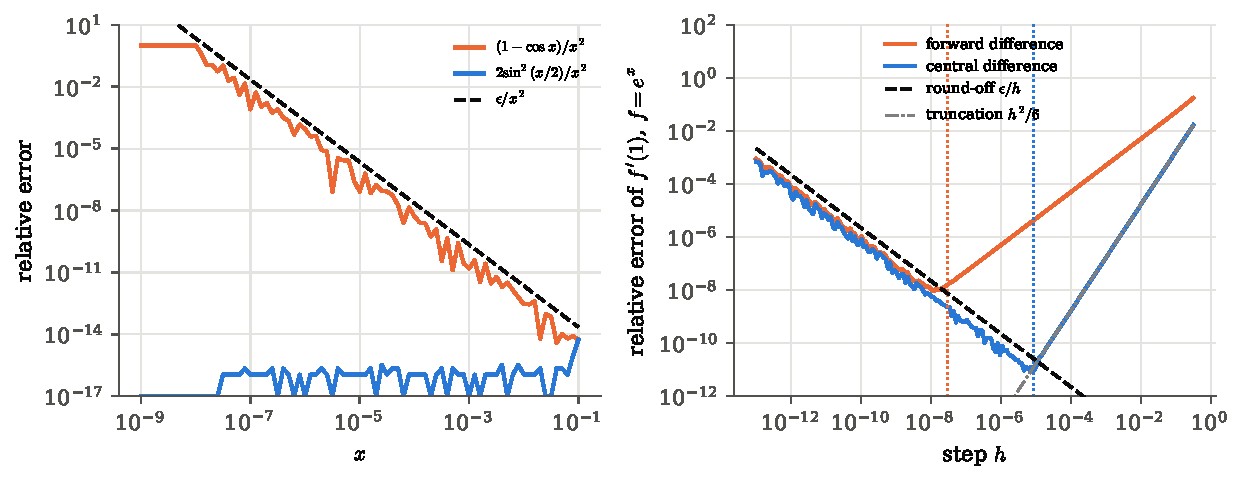
\includegraphics[width=\linewidth]{figures/chT0/08_trust_digits.pdf}
\caption{Where digits go. Left: relative error of $(1-\cos x)/x^2$ computed naively (orange) and as $2\sin^2(x/2)/x^2$ (blue). The naive form loses digits along the dashed line $\epsilon/x^2$ and is useless below $x\approx10^{-8}$; the rewritten form stays at the rounding floor. Right: relative error of the numerical derivative of $e^x$ against the step $h$, for the forward and central differences, as the root-mean-square over $101$ points between $0.5$ and $1.5$. To the right of each minimum the truncation error grows (grey line, $h^2/6$ for the central difference); to the left the round-off error grows as $\epsilon/h$ (dashed). Dotted verticals: the best steps predicted by \eqref{T0a:eq:hopt-central} and its forward analogue.}
\label{T0a:fig:trust-digits}
\end{figure}

\subsection{Derivatives: the step that is neither too large nor too small}
\label{T0a:sec:trust-deriv}

Fisher matrices (\cref{ch:10}), emulators (\cref{9c:sec:emu}) and Newton's method all need derivatives of functions that are known only as code. The obvious approach is the definition of the derivative with a small but finite step $h$. How small? Intuition says ``as small as possible'', and \cref{T0a:fig:trust-digits} (right) shows that intuition to be wrong: the error falls as $h$ shrinks, reaches a minimum, and then rises again. Two errors compete, and the best step is where they balance.

\paragraph{The truncation error.} Take the \newterm{central difference} $D(h)=[f(x+h)-f(x-h)]/2h$. Taylor's theorem gives $f(x\pm h)=f\pm hf'+\tfrac12h^2f''\pm\tfrac16h^3f'''+\dots$, all derivatives at $x$. Subtracting the two expansions cancels the even powers, and dividing by $2h$ leaves
\begin{equation}
  D(h)=f'(x)+\frac{h^2}{6}f'''(x)+O(h^4).
  \label{T0a:eq:central}
\end{equation}
The error $h^2f'''/6$ shrinks as $h$ shrinks: this is the part intuition sees.

\paragraph{The round-off error.} The two function values are computed with relative errors of order $\epsilon$, so each is off by up to about $\epsilon\abs f$, and in the worst case the two errors have opposite signs and add. Their difference is then off by $2\epsilon\abs f$, and dividing by $2h$ leaves $\epsilon\abs f/h$. This part \emph{grows} as $h$ shrinks: for a tiny $h$, $f(x+h)$ and $f(x-h)$ are nearly equal, and their difference is the cancellation of \eqref{T0a:eq:cancel}.

\paragraph{The balance.} The total error and its minimum follow in three lines:
\begin{align}
  E(h)&\eqby{1}\frac{\epsilon\abs f}{h}+\frac{h^2}{6}\abs{f'''},
  \nonumber\\
  \frac{\dd E}{\dd h}&\eqby{2}-\frac{\epsilon\abs f}{h^2}+\frac{h}{3}\abs{f'''}=0
  \quad\Longrightarrow\quad
  h_{\rm opt}\eqby{3}\Bigl(\frac{3\epsilon\abs f}{\abs{f'''}}\Bigr)^{1/3}\sim\epsilon^{1/3},
  \nonumber\\
  E(h_{\rm opt})&\eqby{4}\frac32\,\frac{\epsilon\abs f}{h_{\rm opt}}\sim\epsilon^{2/3}.
  \label{T0a:eq:hopt-central}
\end{align}
\begin{explain}
  \item Round-off plus truncation, the two estimates above.
  \item The smallest error is where the slope of $E$ vanishes.
  \item Multiply by $3h^2/\abs{f'''}$: $h^3=3\epsilon\abs f/\abs{f'''}$, and take the cube root.
  \item At $h_{\rm opt}$, $\frac{h^2}6\abs{f'''}=\frac{h^3}{6h}\abs{f'''}=\frac{3\epsilon\abs f}{6h}=\frac12\,\frac{\epsilon\abs f}{h}$: the truncation term is half the round-off term, and the sum is $\tfrac32$ of it. Since $h_{\rm opt}\sim\epsilon^{1/3}$, this is $\epsilon/\epsilon^{1/3}=\epsilon^{2/3}$.
\end{explain}
For $f=e^x$, where $f=f'''$, the best step is $(3\epsilon)^{1/3}=\TzHcenPred$ and the best relative error about $\epsilon^{2/3}\approx\TzErrCenPred$: two-thirds of the sixteen digits, about ten, survive. The same reasoning for the \newterm{forward difference} $[f(x+h)-f(x)]/h=f'+\tfrac12hf''+\dots$, whose truncation error is first order in $h$, gives $E=2\epsilon\abs f/h+\tfrac12h\abs{f''}$, $h_{\rm opt}=2\sqrt{\epsilon\abs f/\abs{f''}}\sim\epsilon^{1/2}$ and an error of order $\epsilon^{1/2}$: only eight digits. The script scans $h$ and finds:

\TzoutPart{firstline=7,lastline=8}{results/chT0/08_trust_out.txt}

The measured best steps sit where \eqref{T0a:eq:hopt-central} puts them. The measured errors are a few times smaller than predicted, because the prediction assumed the worst case, with the two rounding errors adding; on average they partly cancel.

\paragraph{The plateau check.} For a function whose third derivative is unknown, \eqref{T0a:eq:hopt-central} cannot be evaluated. The practical test is to compute the derivative for steps a factor of ten apart and look for a \newterm{plateau}, a range of $h$ over which the result does not change:

\TzoutPart{firstline=9,lastline=16}{results/chT0/08_trust_out.txt}

The exact value is $e=\TzExactE$. From $h=10^{-2}$ to $10^{-4}$ the digits settle (truncation shrinking a hundredfold per step); at $h=10^{-5}$ and $10^{-6}$ the results agree with each other to ten digits; below that, round-off takes over, and at $h=10^{-12}$ only four digits survive. The digits that stay fixed while $h$ changes by a factor of ten are the ones to trust.

The book chooses its steps in exactly this spirit. The emulator of \cref{9c:sec:emu-build} replaces CAMB by a second-order Taylor expansion in the six cosmological parameters, and its first derivatives are central differences with a fixed step for each parameter:

\pyfile[firstline=57,lastline=60,firstnumber=57]{code/ch09/lib_cmbemu.py}{Central differences of $\ln C_\ell$, one parameter at a time}

Line 57 builds a diagonal matrix whose row $i$ moves parameter $i$ alone by its step (the array \texttt{STEPS}, set on line 29 of the same file to $0.02$ in $\ln(10^{10}A_s)$, $0.01$ in $n_s$, $0.5$ in $H_0$, and so on). Lines 58--59 run CAMB at each shifted point, and line 60 is \eqref{T0a:eq:central}. These steps are far larger than $\epsilon^{1/3}$, and rightly so. CAMB's output is not accurate to sixteen digits but to perhaps six, so its $\epsilon$ is about $10^{-6}$, and \eqref{T0a:eq:hopt-central} then asks for steps of order $10^{-2}$ in relative terms. \Cref{10a:sec:numderiv-errors} redoes the balance with such a ``code noise'' and with the four-point rule, and \cref{10a:sec:numderiv-camb} runs the plateau check on CAMB itself, multiplying all six steps by factors from $\tfrac1{64}$ to $4$ and confirming that the forecast does not move over the middle of that range. \emph{The lesson: a numerical derivative is trustworthy only on a plateau; find it by changing $h$ by factors of ten.}

\subsection{Integrals, roots and minima: what the black boxes report}
\label{T0a:sec:trust-boxes}

\texttt{quad}, \texttt{brentq} and \texttt{minimize} (\cref{T0a:sec:scipy}) are iterations that stop when an internal test is satisfied. Each one reports something about its own reliability, and each can be fooled. The three ways they go wrong are different: \texttt{quad} can be confidently wrong, \texttt{brentq} refuses loudly, and \texttt{minimize} stops quietly.

\paragraph{\texttt{quad} is only as good as the points it looked at.} \texttt{quad} returns a value and an error estimate (\cref{T0a:sec:quad}). The estimate is the disagreement between two integration rules applied to the same function values, and so it says nothing about regions where the function was never evaluated. The script integrates a Gaussian of width $0.01$ centred at $37.3$, whose integral is exactly $1$, over $[0,100]$, and then tries four remedies:

\TzoutPart{firstline=17,lastline=17}{results/chT0/08_trust_out.txt}

Over $[0,100]$ \texttt{quad} first applies a $21$-point rule to the whole interval. No point lands within the peak, every value is zero or astronomically small, both rules agree on zero, and \texttt{quad} reports $\TzQuadMiss$ with a claimed error of $\TzQuadMissErr$. Tightening the tolerance changes nothing, because by \texttt{quad}'s own estimate the answer is already exact. Telling it that something happens at $37.3$, with \texttt{points=[37.3]}, still fails, and instructively: the peak now sits on the boundary between two pieces, and the integration rules never evaluate the function at the ends of a piece. An interval exactly as wide as the peak, \texttt{points=[37.25, 37.35]}, nearly works, and yet the answer is too small by $5.7\times10^{-7}$ while the claimed error is $10^{-9}$: the missing amount is the probability beyond $\pm5\sigma$ (twice the $\TzPfive$ of \cref{T0a:sec:stats}), which lives in the two long outer pieces where \texttt{quad} once again saw nothing. Only an interval that contains the whole peak with room to spare gives $\TzQuadHit$.

The book's integrals are chosen with this in mind: the limits and break points are put where the function lives. The posterior mean of a location parameter with a Student-$t$ likelihood, in the self-normalised importance-sampling study of \cref{6b:sec:self-norm}, is one ratio of two integrals:

\pyfile[firstline=114,lastline=117,firstnumber=114]{code/ch06/27_importance.py}{Integration limits wide enough for heavy tails, and a larger subdivision limit}

Line 115 is the likelihood of three data points at $-4$, $0.5$ and $1$, a product of three $t$ densities with three degrees of freedom. The range $[-60,60]$ is far wider than the data, because $t$ tails fall only as a power of the distance and a short range would cut off a noticeable part of the integral; \texttt{limit=400} lets \texttt{quad} subdivide up to $400$ times instead of the default $50$, so that it can resolve the structure near the data within that wide range. The checks for any \texttt{quad} result follow from the example: plot the integrand once; tighten \texttt{epsabs} and \texttt{epsrel} and see whether the value moves; split the range or change its ends and see whether the value moves. A value that moves was never as accurate as claimed.

\paragraph{\texttt{brentq} needs a bracket, and says so.} \texttt{brentq(f, a, b)} requires $f(a)$ and $f(b)$ to have opposite signs (\cref{T0a:sec:roots}). If they do not, it stops at once:

\TzoutPart{firstline=18,lastline=19}{results/chT0/08_trust_out.txt}

On $[0,1]$ the function $x^2-2$ is negative at both ends, so there is no guaranteed root and \texttt{brentq} refuses; on $[0,2]$ it finds $\sqrt2$ to fourteen digits. This failure is friendly. The care goes into choosing the bracket so that it contains exactly the root wanted: the exact binomial interval of \cref{T0a:sec:pit-float} (lines 40--41 of that excerpt) brackets the lower end between $10^{-6}$ and the estimate $z/N$, and the upper end between $z/N$ and $1-10^{-6}$, because each tail probability crosses its target exactly once on its own side of the estimate.

\paragraph{\texttt{minimize} can stop early, and reports it only if asked.} A minimiser stops when its steps become small, when it runs out of iterations, or when it can no longer find a way downhill. Only the first is success. The script minimises the five-dimensional Rosenbrock function, a long curved valley whose minimum is at $(1,1,1,1,1)$, twice:

\pyfile[firstline=105,lastline=112,firstnumber=105]{code/chT0/08_trust.py}{A minimiser stopped early, and one allowed to finish}

Line 107 runs Nelder--Mead with at most $200$ iterations, line 108 runs BFGS with the exact gradient, and lines 109--112 print, for each, the flag \texttt{success}, the point found, and the length of the gradient there:

\TzoutPart{firstline=20,lastline=21}{results/chT0/08_trust_out.txt}

The first result looks like an answer, a point with a function value of $\TzNMfun$, but \texttt{success} is \texttt{False}, the message says the iteration limit was reached, and the gradient there has length $\TzNMgrad$, far from zero. At a true minimum the gradient vanishes, as it does for BFGS, $\TzBFGSgrad$. Three checks catch an early stop: read \texttt{res.success} and \texttt{res.message}; evaluate the gradient (numerically if need be) at \texttt{res.x}; and restart from \texttt{res.x}, or from a different starting point, to see whether the answer moves. For a likelihood, also check that the curvature there gives a sensible error bar (\cref{ch:03}).

\subsection{Linear algebra: the condition number}
\label{T0a:sec:trust-linalg}

\paragraph{The question.} Solving $A\bm x=\bm b$ is the most common linear-algebra task in the book: every $\chi^2$, every Gaussian likelihood and every Fisher matrix contains one. The data $\bm b$ is never exact: it carries at least rounding error, usually measurement noise. How much does a small relative change of $\bm b$ change $\bm x$?

\paragraph{The smallest example.} Take $A=\mathrm{diag}(1,\,10^{-6})$. The equation splits into $x_1=b_1$ and $x_2=10^6\,b_2$. A change of $\bm b$ by $10^{-16}$ in its second component changes $x_2$ by $10^{-10}$, while $\bm x$ itself may be of order $1$: a relative change $10^{6}$ times that of $\bm b$. The matrix stretches some directions a million times more than others, and inverting it magnifies whatever lies along the weak direction. That ratio of stretches is the whole story.

\paragraph{The general bound.} For any perturbation $\delta\bm b$ the solution changes by $\delta\bm x=A^{-1}\delta\bm b$. Write $\norm{A}$ for the largest factor by which $A$ stretches any vector (its largest singular value, which for a symmetric positive-definite matrix is its largest eigenvalue), so that $\norm{A^{-1}}$ is one over the smallest. Then
\begin{align}
  \frac{\norm{\delta\bm x}}{\norm{\bm x}}
  &\eqby{1}\frac{\norm{A^{-1}\delta\bm b}}{\norm{\bm x}}
   \relby{2}{\le}\frac{\norm{A^{-1}}\,\norm{\delta\bm b}}{\norm{\bm x}}
   \relby{3}{\le}\norm{A^{-1}}\,\norm{A}\,\frac{\norm{\delta\bm b}}{\norm{\bm b}}
   \equiv\kappa(A)\,\frac{\norm{\delta\bm b}}{\norm{\bm b}} .
  \label{T0a:eq:cond}
\end{align}
\begin{explain}
  \item $A(\bm x+\delta\bm x)=\bm b+\delta\bm b$ and $A\bm x=\bm b$ give $\delta\bm x=A^{-1}\delta\bm b$.
  \item No vector is stretched by $A^{-1}$ more than $\norm{A^{-1}}$.
  \item $\norm{\bm b}=\norm{A\bm x}\le\norm A\,\norm{\bm x}$, so $1/\norm{\bm x}\le\norm A/\norm{\bm b}$.
\end{explain}
The \newterm{condition number} $\kappa(A)=\norm A\,\norm{A^{-1}}$ is the ratio of the largest to the smallest stretch, $\lambda_{\max}/\lambda_{\min}$ for a symmetric positive-definite matrix, and $10^6$ in the example. NumPy computes it as \texttt{np.linalg.cond(A)}. Since $\delta\bm b$ is at least rounding, of relative size $\epsilon$, the solution can carry a relative error up to $\kappa\epsilon$. In digits: \emph{about $\log_{10}\kappa$ of the sixteen digits are lost}. The tour of \cref{T0a:sec:linalg} solved a $10\times10$ Hilbert system, whose condition number is $\TzHilbCond$: thirteen digits lost, three left. The recovered $\bm x$ was indeed wrong by $\TzHilbErr$, inside the bound $\kappa\epsilon/2\approx2\times10^{-3}$, whether computed with \texttt{solve} or with \texttt{inv}. No algorithm can do better than the problem allows. What \texttt{solve} does achieve is a tiny residual, $\TzHilbResSolve$: its $\bm x$ solves a problem extremely close to the one posed, which is the most any method can promise. \texttt{inv} followed by a product does not even achieve that ($\TzHilbResInv$), the second reason, after speed, for the rule ``solve, do not invert''.

The book measures condition numbers where it matters. The mode-coupling matrix of the pseudo-$C_\ell$ method (\cref{8b:sec:invert}) must be inverted for every mask, and the script that builds it records its condition number for each:

\pyfile[firstline=74,lastline=75,firstnumber=74]{code/ch08/22_coupling.py}{The condition number of the coupling matrix, measured}

Line 74 keeps the multipoles $\ell\ge2$ (the monopole and dipole are removed from the maps), and line 75 computes $\kappa$. For the full sky it is $\EightBcondFull$, for the $70\%$ cap $\EightBcondCapSeventy$: harmless. For the $30\%$ and $10\%$ caps it is $\EightBcondCapThirty$ and $\EightBcondCapTen$, beyond $1/\epsilon$: all sixteen digits lost, the matrix singular to machine precision. \Cref{8b:sec:invert} explains why, and what is done instead (binning, which keeps only the well-determined combinations).

\paragraph{Cholesky failing is a message.} \texttt{np.linalg.cholesky} succeeds only for a symmetric matrix whose eigenvalues are all positive, and stops with \texttt{LinAlgError} otherwise. When a covariance matrix fails it, the matrix is telling us something. The script estimates the covariance of a $50$-bin data vector from $30$ and from $200$ simulations:

\TzoutPart{firstline=22,lastline=23}{results/chT0/08_trust_out.txt}

Why does $30$ fail? The sample covariance $\hat\Cmat=\frac1{n-1}\sum_{i=1}^n(\bm x_i-\bar{\bm x})(\bm x_i-\bar{\bm x})\T$ is a sum of $n$ matrices of the form $\bm u\bm u\T$, each of which stretches only along its own vector $\bm u$. And the $n$ vectors $\bm x_i-\bar{\bm x}$ are not independent: they sum to zero, so any one is minus the sum of the others. So $\hat\Cmat$ stretches at most $n-1$ directions and is exactly zero along the remaining $p-(n-1)$. With $n=30$ and $p=50$ the rank is $29$, twenty-one eigenvalues are zero (computed as $\pm10^{-15}$, rounding around zero), and the Cholesky factor does not exist. With $n=200$ all $50$ eigenvalues are positive and it succeeds. The failure says: not enough simulations to estimate this covariance. Even when $n>p$ the inverse of $\hat\Cmat$ is biased, and the Hartlap factor $(n-p-2)/(n-1)$ of \cref{8b:sec:hartlap} corrects it; \cref{8b:sec:nsims} asks how many simulations are enough.

A script that might meet such a matrix catches the error instead of crashing. The bootstrap of Hubble's 1929 galaxies (\cref{11c:sec:hubble-compare}) refits a model with a solar-motion term to each resampled set of twenty-four galaxies:

\pyfile[firstline=119,lastline=126,firstnumber=119]{code/ch11/08_hubble1929.py}{A resample whose fit is singular is recorded as missing, not hidden}

Line 120 draws $N$ galaxy indices with replacement, and line 121 refits the simple model. A resample can repeat a few galaxies so often that their directions on the sky no longer determine the four parameters of the fit, and the linear solve inside \texttt{fit\_solar} (\texttt{np.linalg.solve} on the normal equations) then fails. Lines 122--125 catch exactly that error and record the resample as \texttt{np.nan}; line 126 removes those before any statistic is formed, and the number removed can be printed. \emph{The lesson: $\log_{10}\kappa$ digits are lost to the matrix; a failed Cholesky factor is a diagnosis, not a nuisance.}

\subsection{Monte Carlo noise: every simulated number has an error bar}
\label{T0a:sec:trust-mc}

A Monte Carlo estimate is an average of $N$ independent draws, so its standard deviation is $\sigma/\sqrt N$, with $\sigma$ the standard deviation of a single draw: the variance of an average is the single-draw variance divided by $N$, derived in \cref{6b:sec:sqrtN}. The rule that follows is simple: every simulated number is quoted with its $\sigma/\sqrt N$, which is estimated from the same draws. The first Monte Carlo of the book, the estimate of $\pi$ from random points in a square (\cref{0a:sec:code}), does exactly that:

\pyfile[firstline=21,lastline=26,firstnumber=21]{code/ch00/06_reproducible_seeds.py}{A Monte Carlo estimate and its standard error, side by side}

Line 24 is the fraction of points inside the quarter disc, line 25 the estimate $\hat\pi=4\times$fraction, and line 26 its standard error: a fraction of $N$ independent yes/no draws has variance $q(1-q)/N$, and multiplying by $4$ multiplies the standard deviation by $4$. With $N=10^6$ the script finds $\hat\pi=\PiHat\pm\PiErr$, which is within one standard error of $\pi$.

\paragraph{Rerunning with a different seed.} The error bar is a prediction: other seeds should scatter by about that much. That prediction can be tested directly. The script estimates $\Prob(Z>2)$ with $N=10^4$ draws for eight different streams:

\TzoutPart{firstline=24,lastline=24}{results/chT0/08_trust_out.txt}

The eight estimates scatter by $\TzQobsFour$ against the predicted $\TzQsigFour$, the agreement expected for eight values, whose own standard deviation is uncertain by about $1/\sqrt{2\times7}\approx27\%$ (\cref{7b:sec:mc-var}). \Cref{T0a:fig:trust-mc} (left) shows the same for $N$ from $10^2$ to $10^6$: the estimates converge onto the exact value inside a band that narrows as $1/\sqrt N$. Each factor of ten in accuracy costs a factor of a hundred in draws.

\paragraph{Common random numbers.} Often the question is not a number but a difference: how much does a probability change when a parameter changes? Two independent Monte Carlo runs each carry their own noise, and the noise of the difference is larger than either. The cure is to run both settings on the \emph{same} random draws. Why that helps follows from the variance of a difference of two estimates $A$ and $B$:
\begin{align}
  \Var(A-B)
  &\eqby{1}\Var A+\Var B-2\Cov(A,B).
  \label{T0a:eq:crn}
\end{align}
\begin{explain}
  \item Expand $\E[(A-B-\E A+\E B)^2]$: the two squares give the variances, and the cross term gives $-2\Cov(A,B)$.
\end{explain}
With independent draws, $\Cov(A,B)=0$ and the variances add. With the same draws, the two estimates rise and fall together, $\Cov(A,B)$ is positive and nearly as large as the variances, and most of the noise cancels in the difference. This is the method of \newterm{common random numbers}. The script compares $\Prob(X>2)$ for $X\sim\Normal(\mu,1)$ at $\mu=0$ and at $\mu=0.1$, repeating the comparison $\TzCrnR$ times with $\TzCrnM$ draws each:

\pyfile[firstline=147,lastline=153,firstnumber=147]{code/chT0/08_trust.py}{The same change estimated with fresh draws, and with the same draws shifted}

Line 151 draws two independent sets of standard Gaussians. Line 152 estimates the change with fresh draws for the second setting; line 153 uses the first set for both settings, shifting it by $\delta=0.1$ for the second. The exact change is $\TzCrnTrue$. Its scatter over the repetitions is $\TzCrnInd$ with independent draws and $\TzCrnCrn$ with common ones, a variance $\TzCrnGain$ times smaller, worth $\TzCrnGain$ times as many draws (\cref{T0a:fig:trust-mc}, right). With independent draws a single comparison measures the change at only $\TzCrnZind$ standard deviations; with common random numbers, at $\TzCrnZcrn$.

The book uses common random numbers wherever it compares settings. The CMB pipeline of \cref{8a:sec:pipeline} computes seven different spectra from the \emph{same} simulated sky, so that the bias of one estimator relative to another is measured to a fraction of a per cent. The simulated Fisher matrices of \cref{12w:sec:mc-fisher} and \cref{12c:sec:deriv} take each derivative from maps that share their random seed, so that the maps differ only through the change of cosmology. \emph{The lesson: quote $\sigma/\sqrt N$ with every simulated number, and compare settings on the same random numbers.}

\begin{figure}[htbp]
\centering
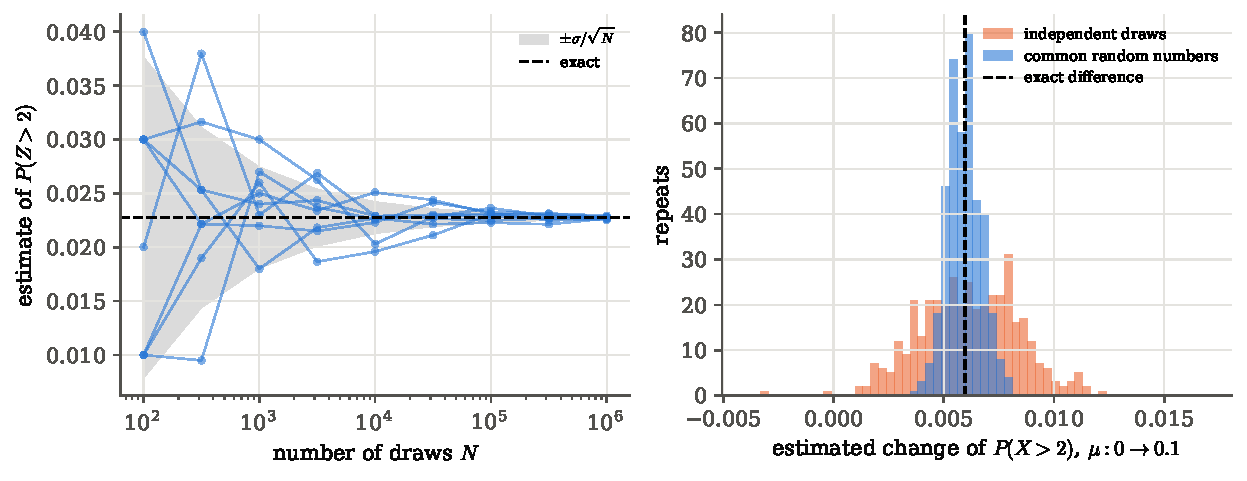
\includegraphics[width=\linewidth]{figures/chT0/08_trust_mc.pdf}
\caption{Monte Carlo noise. Left: estimates of $\Prob(Z>2)$ from eight independent streams (blue lines) against the number of draws; the grey band is the predicted $\pm\sigma/\sqrt N$ around the exact value (dashed). Right: the estimated change of $\Prob(X>2)$ when the mean moves from $0$ to $0.1$, over $400$ repetitions of $10^4$ draws each. Independent draws for the two settings (orange) scatter about three times more widely than common random numbers (blue) around the exact change (dashed).}
\label{T0a:fig:trust-mc}
\end{figure}

\subsection{Convergence: change the resolution until nothing changes}
\label{T0a:sec:trust-conv}

Every computation in the book has a resolution: a grid spacing, a number of points per axis, a HEALPix $N_{\rm side}$, a maximum multipole $\ell_{\max}$, a number of simulations or of chain steps. The answer at finite resolution differs from the answer the resolution is meant to approximate. The test is a \newterm{convergence study}: compute at two or three resolutions, and accept the answer only when it changes by less than its other errors.

\paragraph{Example: the trapezoid rule.} The integral $\int_0^\pi\sin x\,\dd x=2$ computed by the trapezoid rule with $n$ intervals:

\TzoutPart{firstline=26,lastline=28}{results/chT0/08_trust_out.txt}

Each halving of the step divides the error by $\TzTrapRatio$, almost exactly $4$. That number is itself information: an error that falls as $h^2$ is what the trapezoid rule should give (for a smooth function the trapezoid value exceeds the integral by $\frac{(b-a)h^2}{12}\overline{f''}$, with $\overline{f''}$ an average of the second derivative, here $-\sin x<0$, hence the negative errors), so the code behaves as its theory says. An error ratio far from the expected one is the sign of a bug or of a function that is not smooth.

\paragraph{Richardson extrapolation.} Knowing that the error falls as $h^2$ allows it to be removed. Write the result with step $h$ as its limit plus the leading error, and do the same for $h/2$:
\begin{align}
  T(h)&\eqby{1}I+ch^2+O(h^4),
  \qquad
  T(h/2)\eqby{2}I+\tfrac14ch^2+O(h^4),
  \nonumber\\
  \frac{4T(h/2)-T(h)}{3}&\eqby{3}\frac{4I+ch^2-I-ch^2}{3}+O(h^4)=I+O(h^4).
  \label{T0a:eq:richardson}
\end{align}
\begin{explain}
  \item The trapezoid error expanded in powers of the step. For a smooth function only even powers appear.
  \item The same with $h$ replaced by $h/2$: the coefficient $c$ is the same, so the $h^2$ term is a quarter as large.
  \item Four times the second line minus the first: the $h^2$ terms cancel and $3I$ remains; divide by $3$.
\end{explain}
The script prints the result:

\TzoutPart{firstline=29,lastline=29}{results/chT0/08_trust_out.txt}

From the two cheap values at $n=8$ and $16$, whose errors are $\TzTrapErrEight$ and $\TzTrapErrSixteen$, the combination gives an error of $\TzRichErr$: about four hundred times smaller than at $n=16$, for no new function evaluations. The four-point derivative of \cref{10a:sec:numderiv-errors} is the same trick applied to \eqref{T0a:eq:central}.

The book's convergence studies follow this pattern. The brute-force evidence of a four-parameter model in \cref{5c:sec:grid-cost} is computed with $n$ points per axis for seven values of $n$:

\pyfile[firstline=50,lastline=57,firstnumber=50]{code/ch05/27_grid_cost.py}{The same integral at seven resolutions, each timed}

Line 50 lists the resolutions, and the loop of lines 52--57 computes the log Bayes factor at each, timing it with \texttt{time.perf\_counter} (\cref{T0a:sec:cost}). The answer moves from $\FiveCGcLnBsmall$ at $n=\FiveCGcNsmall$ to $\FiveCGcLnBmid$ at $n=\FiveCGcNmid$ and $\FiveCGcLnBmax$ at $n=\FiveCGcNmax$, against the exact $\FiveCGcExact$: only the finest grids have converged. \Cref{8a:sec:res-conv} does the same with the number of simulated skies, watching the estimated bias and error bar settle inside the band $\pm\sigma/\sqrt N$. \emph{The lesson: an answer is converged when doubling the resolution changes it by less than its other errors.}

\subsection{Validation: test the code where the answer is known}
\label{T0a:sec:trust-valid}

The checks so far estimate the size of an error. None of them catches a plain mistake in the code: a sign, a factor of two, a wrong index. Those are caught by one habit, used throughout the book: before a method is trusted on a problem with no known answer, it is run on a problem with one. The Monte Carlo variance of simulated $\Chat$ is compared with the cosmic variance $2\Cell^2/(2\ell+1)$ before simulations are used for masked skies (\cref{7b:sec:mc-var}); the exact binomial interval found by root finding is compared with the closed formula in terms of the beta distribution (\cref{T0a:sec:pit-float}); the healpy round trip of \cref{T0a:sec:blackbox} must return the spectrum that went in; the Fisher forecast is checked against an MCMC run on the same likelihood (\cref{ch:10}).

A comparison can be written into the script as an \texttt{assert}: \texttt{assert condition} does nothing when the condition is true and stops the script with an error when it is false. The tiny-image study of \cref{12c:sec:tiny} enumerates every one of the $2^9=512$ black-and-white $3\times3$ images and checks three facts about each:

\pyfile[firstline=29,lastline=38,firstnumber=29]{code/ch12/c01_tiny.py}{Three identities checked on every one of 512 images}

Line 30 runs through all $512$ patterns of nine bits, line 31 turns each into a $3\times3$ image, and lines 32--33 count its pieces and holes and compute its Euler characteristic with the book's own functions. Line 34 asserts the Euler relation $\chi=\beta_0-\beta_1$; lines 36--37 assert that scikit-image's independent implementation finds the same number of pieces and the same $\chi$. If any of the $1536$ checks failed, the script would stop at that image. These are exact integer comparisons, so \texttt{==} is right here; between real numbers the comparison is made with a tolerance (\cref{T0a:sec:trust-float}).

The census of \cref{T0a:sec:census} counts how often the book writes such checks into its code: $\TzAsserts$ \texttt{assert} statements in $\TzAssertFiles$ files, and $\TzCheckCalls$ calls of \texttt{np.isclose}, \texttt{np.allclose} and similar comparison functions in $\TzCheckFiles$. That is a small number, and it understates the validation, because most of the book's checks are not asserts. They are a figure in which the simulation is drawn over the analytic curve (the black dashed \texttt{theory\_line} of \cref{T0a:sec:plots}), or a pair of numbers saved by the script and quoted side by side in the text. A comparison in a figure or in the text is read by a person, who notices a discrepancy that no one thought to assert. \emph{The lesson: a method is trusted where its answer is unknown only after it has reproduced an answer that is known.}

\begin{inpractice}[Verification first, then research]
The same simulation code plays two roles. Run on an ideal full-sky Gaussian field, it \emph{verifies}: its variance of $\Chat$ must reproduce $2\Cell^2/(2\ell+1)$ within its Monte Carlo error. Run with a mask, a beam and inhomogeneous noise, where no formula exists, it is the \emph{research instrument}: the covariance it produces feeds a likelihood (\cref{ch:08}). Research codes follow this order as a rule, and publish their validation tests next to their results.
\end{inpractice}

\subsection{The decision rule: is a difference real?}
\label{T0a:sec:trust-decide}

Every check above ends with a comparison of two numbers: a simulation and a formula, two resolutions, two methods, two settings. They never agree exactly. When is a difference real, and when is it noise? The rule is the one every physicist uses for measurements. Collect the uncertainty of each number from every source, numerical and Monte Carlo, add the independent ones in quadrature, and divide the difference by the result:
\begin{equation}
  z=\frac{\abs{x_1-x_2}}{\sqrt{\sigma_1^2+\sigma_2^2}},
  \qquad
  \sigma_i^2=\sigma_{i,\rm MC}^2+\sigma_{i,\rm num}^2 .
  \label{T0a:eq:zscore}
\end{equation}
If the two numbers really estimate the same quantity and the errors are roughly Gaussian, $z$ is the absolute value of a standard Gaussian variable: below $1$ two times in three, below $2$ nineteen times in twenty, above $3$ about once in four hundred. So $z\lesssim2$ means ``consistent''; $z$ between $2$ and $3$ means ``look again'', with more draws or another seed; $z\gtrsim3$, in a single planned comparison, means that the difference is real, which may mean a bug. When many comparisons are made at once, a few values of $z$ near $2$ to $3$ are expected by chance alone, exactly the look-elsewhere problem of \cref{4b:sec:lee}.

\paragraph{Example: the Monte Carlo variance at the quadrupole.} \Cref{7b:sec:mc-var} estimates the variance of $\Chat$ from $\SBNsim$ simulated skies and compares it with the cosmic variance $2\Cell^2/(2\ell+1)$. At $\ell=2$ the ratio of the two is $\SBvrTwo$, a $2\%$ excess. Is the formula wrong, or the simulation, or neither? The analytic answer has no numerical error worth mentioning, and the simulated one has the Monte Carlo error derived there, $\SBerrTwo$ in units of the ratio. So
\[
  z=\frac{\SBvrTwo-1}{\SBerrTwo}\approx\TzZcv ,
\]
well inside the range of chance: neither is wrong. Had the excess been $10\%$, $z$ would have been about $7$, and the code would have been searched for the bug.

\paragraph{Example: a change seen with and without common random numbers.} In \cref{T0a:sec:trust-mc}, a single comparison of $\Prob(X>2)$ at $\mu=0$ and $\mu=0.1$ with independent draws measures the true change $\TzCrnTrue$ against a noise of $\TzCrnInd$: $z\approx\TzCrnZind$, a ``look again''. Over the $\TzCrnR$ repeats, $\TzCrnFracIndBelow\%$ of such single comparisons fall short of $3\sigma$, so one of them alone often would not establish that the probability changed at all. With common random numbers the noise is $\TzCrnCrn$ and $z\approx\TzCrnZcrn$, and $\TzCrnFracCrnBelow\%$ fall short: a difference beyond doubt, from the same number of draws.

\begin{keyidea}[When a computed number can be trusted]
A computed number is trusted to the extent that its error budget is known: rounding ($\epsilon$ times the amplification of cancellation or of the condition number), the method (step size, tolerance, resolution, checked by changing them), and Monte Carlo noise ($\sigma/\sqrt N$, checked by changing the seed). A difference is real when it is large compared with the combined budget, $z\gtrsim3$; and a method is trusted on an unknown answer only after it has reproduced a known one.
\end{keyidea}

\Cref{T0a:tab:checklist} collects the checks in the form in which they are needed: a symptom, the check that diagnoses it, the fix, and a place in the book where it is done.

\begin{table}[htbp]
\centering
\small
\renewcommand{\arraystretch}{1.15}
\begin{tabularx}{\linewidth}{@{}>{\raggedright\arraybackslash}p{2.9cm}
                               >{\raggedright\arraybackslash}X
                               >{\raggedright\arraybackslash}p{3.1cm}
                               >{\raggedright\arraybackslash}p{2.1cm}@{}}
\toprule
symptom & check & fix & in the book\\\midrule
\texttt{==} between real numbers fails & print the difference; compare it with $\epsilon$ times the size & \texttt{np.isclose}, or a relative tolerance & \cref{T0a:sec:pit-float,T2a:sec:dm}\\
digits lost in a small difference & count the leading digits that cancel, \eqref{T0a:eq:cancel} & rewrite the formula; subtract the large common part first & \cref{T0a:sec:trust-float,3a:sec:var-python}\\
derivative changes with the step & scan $h$ by factors of ten; look for a plateau & a step on the plateau; four-point rule & \cref{10a:sec:numderiv-camb,9c:sec:emu-build}\\
integral with a tiny claimed error & plot the integrand; tighten the tolerance; change the range & limits and \texttt{points} where the function lives & \cref{6b:sec:self-norm}\\
\texttt{brentq} raises \texttt{ValueError} & evaluate $f$ at both ends & a bracket with a sign change around the wanted root & \cref{4b:sec:ci-intentions}\\
minimiser result looks plausible & \texttt{res.success}, \texttt{res.message}, gradient at \texttt{res.x} & more iterations; restart from \texttt{res.x}; a gradient-based method & \cref{T0a:sec:minimize}\\
solution of $A\bm x=\bm b$ unstable & \texttt{np.linalg.cond(A)}; $\log_{10}\kappa$ digits are lost & \texttt{solve}, not \texttt{inv}; bin or regularise & \cref{8b:sec:invert}\\
\texttt{cholesky} raises \texttt{LinAlgError} & eigenvalues of the matrix; rank against the number of simulations & more simulations; Hartlap factor & \cref{8b:sec:hartlap,8b:sec:nsims}\\
simulated number without an error bar & $\sigma/\sqrt N$ from the same draws; another seed & quote it; increase $N$ & \cref{6b:sec:sqrtN,7b:sec:mc-var}\\
noisy difference of two simulations & scatter of the difference over seeds & common random numbers & \cref{8a:sec:pipeline,12w:sec:mc-fisher}\\
answer depends on grid, $N_{\rm side}$, $\ell_{\max}$ & halve the step or double the size & finer resolution; Richardson extrapolation & \cref{5c:sec:grid-cost,8a:sec:res-conv}\\
a new method on a new problem & run it where the answer is known & find the bug before trusting the result & \cref{7b:sec:mc-var,12c:sec:tiny}\\
two numbers disagree & $z$ of \eqref{T0a:eq:zscore} with all errors & $z\lesssim2$: noise; $z\gtrsim3$: real, or a bug & \cref{7b:sec:mc-var}\\
\bottomrule
\end{tabularx}
\caption{Is the number real? Thirteen symptoms, the check that diagnoses each, the usual fix, and a place in the book where it is done.}
\label{T0a:tab:checklist}
\end{table}
\section{When sixteen digits are not enough: mpmath}
\label{T0a:sec:precision}

A double-precision number carries about sixteen significant digits and spans magnitudes from about $10^{-308}$ to $10^{308}$ (\cref{T0a:sec:trust-float}). For almost everything in the book that is ample. Occasionally it is not, and the failure has a recognisable shape: a probability so small that it underflows to zero, a sum whose terms cancel so completely that no digit of the answer survives, a factorial or a Gamma function so large that it overflows. The library \newterm{mpmath} computes with as many digits as we ask for, and the question is when to reach for it, how many digits to ask for, and what it costs.

\paragraph{The smallest example: the significance of a large excess.} The one-sided $p$-value of a $z\sigma$ excess is the Gaussian tail $\Prob(Z>z)$ (\cref{ch:04}). There are three ways to compute it in SciPy: \texttt{1 - norm.cdf(z)}, \texttt{norm.sf(z)} (the survival function, which computes the tail directly) and \texttt{norm.logsf(z)}, its natural logarithm. The script \pyname{code/chT0/09_mpmath.py} compares all three with mpmath at fifty digits:

\TzoutPart{firstline=1,lastline=8}{results/chT0/09_mpmath_out.txt}

At $5\sigma$, the discovery threshold of particle physics, all three are fine: even the naive \texttt{1 - cdf} is accurate to a relative $\TzNaiveRelFive$. At $8\sigma$ the naive form is already $7\%$ wrong, and from $\TzNaiveZero\sigma$ on it returns exactly $0$. The reason is the spacing of storable numbers just below $1$, which is $\epsilon/2\approx1.1\times10^{-16}$: the cdf is stored as the nearest of these, so a tail much smaller than $10^{-16}$ cannot be represented as ``$1$ minus something'' at all. \texttt{sf} avoids the subtraction and stays accurate down to about $10^{-300}$, but at $\TzSfZero\sigma$ the tail itself, about $10^{-316}$, is below the smallest number with full precision, $\TzTiny$, and the function returns $0$. \texttt{logsf} never forms the tiny number: it computes $\ln\Prob(Z>z)$ directly, a modest negative number, and agrees with mpmath to every printed digit all the way to $40\sigma$, where $\log_{10}\Prob=\TzLogsfForty$ (\cref{T0a:fig:mpmath}, left). The naive choice fails silently at $8\sigma$; the good choice, \texttt{sf} or \texttt{logsf}, costs nothing. \emph{The lesson: rewrite first; reach for more digits only when no rewriting will do, and then mostly to check.}

\begin{figure}[htbp]
\centering
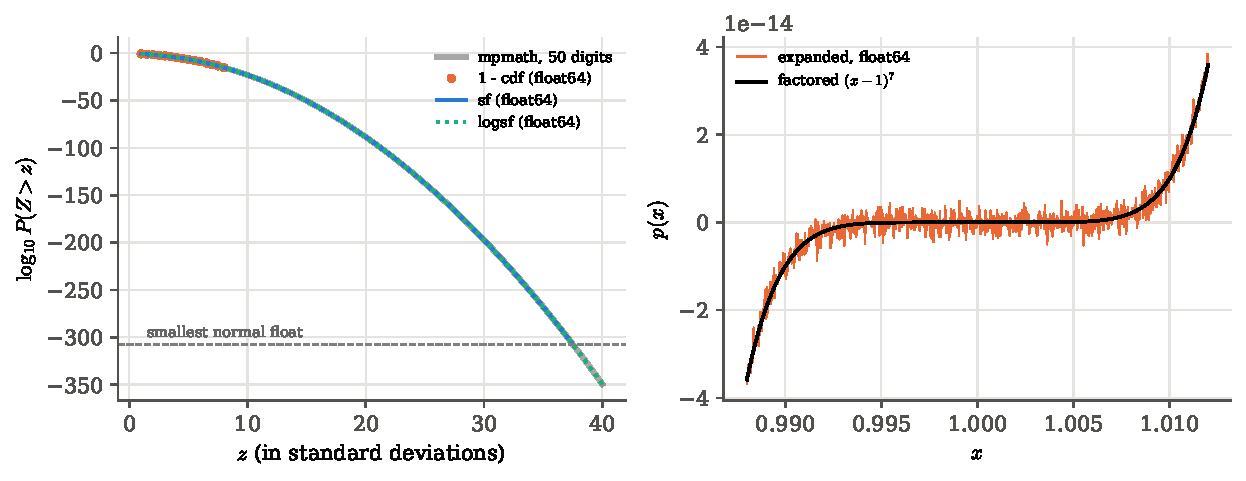
\includegraphics[width=\linewidth]{figures/chT0/09_mpmath.pdf}
\caption{Where double precision breaks. Left: $\log_{10}\Prob(Z>z)$ from mpmath at fifty digits (thick grey) and from three float64 routes. \texttt{1 - cdf} (orange points) stops near $8.5\sigma$, \texttt{sf} (blue) at $38\sigma$, where the tail falls below the smallest normal float (dashed); \texttt{logsf} (dotted) follows mpmath to the end. Right: the polynomial $(x-1)^7$ near its root, evaluated from its expanded coefficients in float64 (orange) and in factored form (black). The expanded form returns rounding noise of size about $10^{-14}$ instead of a smooth curve.}
\label{T0a:fig:mpmath}
\end{figure}

\subsection{Log space first}
\label{T0a:sec:logspace}

Most overflows and underflows in statistics come from products of many factors (likelihoods), from factorials and Gamma functions (binomial and Poisson probabilities, normalising constants), and from exponentials of large numbers (evidences, Boltzmann weights). All of them disappear when the computation is done with logarithms, which turn products into sums and keep every intermediate number of modest size. SciPy supplies the two tools that make this painless.

\paragraph{\texttt{gammaln}.} \texttt{scipy.special.gammaln(x)} returns $\ln\Gamma(x)$ without forming $\Gamma(x)$. Since $n!=\Gamma(n+1)$, $\ln 200!$ is \texttt{gammaln(201)}, which is $\TzLnFact$, while $200!$ itself, about $10^{375}$, overflows (\cref{T0a:sec:special}). A ratio of Gamma functions is the exponential of a difference of \texttt{gammaln}s. The bias factor $c_4(N)=\sqrt{2/(N-1)}\,\Gamma(N/2)/\Gamma\bigl((N-1)/2\bigr)$ of the sample standard deviation (\cref{3a:sec:n-minus-one}) is computed this way:

\pyfile[firstline=68,lastline=68,firstnumber=68]{code/ch03/04_sample_variance.py}{A ratio of Gamma functions as the exponential of a difference of logarithms}

For $N=5$ the direct ratio would be harmless, but $\Gamma(N/2)$ overflows above $N\approx344$, while the line as written works for any $N$: the logarithms stay of order $N\ln N$, and their difference, the logarithm of $c_4$, is close to zero.

\paragraph{\texttt{logsumexp}.} An evidence, a mixture density or a normalisation is a sum of exponentials, $\ln\sum_ie^{a_i}$, and the $a_i$ are log-likelihoods, often in the hundreds or thousands. For $a_1=-1000$ and $a_2=-1001$, \texttt{np.exp} underflows both to $0$ and the logarithm of the sum is $-\infty$. Factoring out the largest term $m=\max_ia_i$ removes the problem:
\begin{align}
  \ln\sum_ie^{a_i}
  &\eqby{1}\ln\Bigl(e^{m}\sum_ie^{a_i-m}\Bigr)
   \eqby{2}m+\ln\sum_ie^{a_i-m} .
  \label{T0a:eq:logsumexp}
\end{align}
\begin{explain}
  \item $e^{a_i}=e^{m}e^{a_i-m}$ for every $i$; take the common factor out of the sum.
  \item The logarithm of a product is the sum of the logarithms, and $\ln e^m=m$.
\end{explain}
Now every exponent $a_i-m$ is at most $0$, the largest term is exactly $1$, nothing overflows, and the terms that underflow are those too small to matter. For the example, $-1000+\ln(1+e^{-1})=-999.687$. \texttt{scipy.special.logsumexp} does exactly this. The posterior probabilities of three competing models in \cref{5c:sec:how-many} are their evidences normalised to sum to one, computed in log space throughout:

\pyfile[firstline=66,lastline=67,firstnumber=66]{code/ch05/25_how_many_bumps.py}{Posterior model probabilities from log-evidences}

Line 66 collects the three log-evidences, for no bump, one bump and two bumps. Line 67 subtracts $\ln\sum_ke^{\ln Z_k}$ from each, which is the logarithm of $Z_k/\sum_jZ_j$, the posterior probability of model $k$ when the three are equally probable a priori. The evidences themselves are never formed. The tail probability above is the same idea in SciPy's distributions: \texttt{logpdf}, \texttt{logcdf} and \texttt{logsf} exist for every distribution, and a likelihood of many data points is built as a sum of \texttt{logpdf} values rather than a product of \texttt{pdf} values, which underflows to zero once there are a few hundred points.

\subsection{Cancellation that cannot be rewritten away}
\label{T0a:sec:mp-cancel}

Sometimes no rewriting is available, because the formula arrives as given. A polynomial from a series expansion or a fit comes as its coefficients, not in factored form. The script takes the polynomial $(x-1)^7$ in its expanded form, $x^7-7x^6+21x^5-35x^4+35x^3-21x^2+7x-1$, evaluates it near $x=1$ by Horner's rule (multiply by $x$, add the next coefficient, repeat), and compares with the factored form:

\TzoutPart{firstline=9,lastline=10}{results/chT0/09_mpmath_out.txt}

At $x=1.01$ the exact value is $10^{-14}$; float64 returns $\TzPolyFloat$, wrong by $20\%$. \Cref{T0a:fig:mpmath} (right) shows the expanded form near the root: not a curve but a band of rounding noise. mpmath with fifteen digits reproduces the float64 answer digit for digit, because it is making the same rounding errors with the same number of digits; with thirty digits it returns $\TzPolyMpThirty$.

\paragraph{How many digits survive?} The question is the one answered for a single subtraction by \eqref{T0a:eq:cancel}, now for a sum of many terms. Suppose each term $t_k$ of a sum $p=\sum_kt_k$ is computed with relative error at most $u$, the working precision: $u\approx\epsilon/2$ in float64, and $u\approx10^{-d}$ when mpmath carries $d$ decimal digits. Then
\begin{align}
  \frac{\abs{\hat p-p}}{\abs p}
  &\eqby{1}\frac{\abs{\sum_kt_k\delta_k}}{\abs{\sum_kt_k}}
   \relby{2}{\le}u\,\frac{\sum_k\abs{t_k}}{\abs{\sum_kt_k}}
   \equiv u\,\kappa ,
  \nonumber\\
  \text{digits trusted}
  &\eqby{3}-\log_{10}(u\kappa)\approx d-\log_{10}\kappa .
  \label{T0a:eq:digits}
\end{align}
\begin{explain}
  \item Each computed term is $t_k(1+\delta_k)$, so the error of the sum is $\sum_kt_k\delta_k$.
  \item The triangle inequality and $\abs{\delta_k}\le u$.
  \item A relative error $10^{-j}$ means $j$ correct digits; with $u=10^{-d}$, $-\log_{10}u=d$.
\end{explain}
The \newterm{condition number} of the sum, $\kappa=\sum_k\abs{t_k}/\abs{\sum_kt_k}$, is the ratio of the size of the terms to the size of the result. For two terms, $a$ and $-b$, it is $(\abs a+\abs b)/\abs{a-b}$, the amplification factor of \eqref{T0a:eq:cancel}; for a linear system it is the $\kappa(A)$ of \eqref{T0a:eq:cond}. The rule reads the same each time: \emph{working digits minus $\log_{10}\kappa$}. (Rounding inside Horner's rule adds a factor of order the number of terms, a fraction of a digit to one digit; the rule is a guide, not a guarantee.)

For the expanded polynomial the terms are the binomial coefficients times powers of $x$, so $\sum_k\abs{t_k}=(x+1)^7$ by the binomial theorem, and
\[
  \kappa=\frac{(x+1)^7}{\abs{x-1}^7}=\Bigl(\frac{2.01}{0.01}\Bigr)^7\approx1.3\times10^{16}
  \quad\text{at }x=1.01,
\]
which the script confirms, $\kappa=\TzPolyKappa$ ($\log_{10}\kappa=\TzPolyLogKappa$). With $d\approx16$ working digits, \eqref{T0a:eq:digits} predicts that \emph{no} digit survives, and indeed none of the float64 answer is right. To keep ten digits we need $d\approx\TzPolyLogKappa+10\approx26$; asking for thirty leaves a margin.

\paragraph{The practical test: $d$ against $2d$.} The condition number is rarely known in advance. The practical rule is to compute the same quantity twice, at $d$ and at $2d$ digits, and keep the digits on which the two agree. Why does this work? The error of the $2d$ result is about $10^{-d}$ times smaller than that of the $d$ result, so the difference between the two is, to a good approximation, the error of the $d$ result itself:

\pyfile[firstline=77,lastline=88,firstnumber=77]{code/chT0/09_mpmath.py}{The same sum at $d$ and at $2d$ digits, and the number of digits on which they agree}

Line 80 sets the working precision to \texttt{dps} decimal digits, and line 81 evaluates the polynomial at $1.01$; line 82 doubles the precision and line 83 evaluates again. The input is given as the string \texttt{"1.01"}, so mpmath reads the decimal number exactly to the working precision; \texttt{mp.mpf(1.01)} would inherit the binary rounding of the float $1.01$. Line 85 converts the relative difference into a number of agreeing digits. The result:

\TzoutPart{firstline=11,lastline=15}{results/chT0/09_mpmath_out.txt}

At $d=10$ and $d=15$ the two results disagree completely: no digit of the $d$-digit answer can be trusted, as \eqref{T0a:eq:digits} predicted for $d<16$. At $d=20$ they agree on $\TzAgreeTwenty$ digits, and at $d=30$ on $\TzAgreeThirty$; the rule, $d-16$, predicted four and fourteen, so it is conservative, because it assumes that all rounding errors line up. \emph{The lesson: the digits that survive a doubling of the precision are the digits to keep.}

\begin{figure}[htbp]
\centering
\begin{tikzpicture}[x=0.17cm,y=0.62cm]
  \foreach \row/\d/\lab in {0/16/{float64, $d\approx16$},1/30/{mpmath, $d=30$},2/50/{mpmath, $d=50$}} {
    \fill[formblue!25] (0,-\row) rectangle (\d,-\row+0.7);
    \fill[bdryred!35] (0,-\row) rectangle ({min(16,\d)},-\row+0.7);
    \draw[black!60] (0,-\row) rectangle (\d,-\row+0.7);
    \node[font=\footnotesize,anchor=east] at (-0.3,-\row+0.35) {\lab};
  }
  \draw[black!50,dashed] (16,0.95) -- (16,-2.2);
  \node[font=\scriptsize,anchor=south,bdryred!80!black] at (8,0.75) {lost: $\log_{10}\kappa\approx16$};
  \node[font=\scriptsize,formblue!70!black] at (23,-1+0.35) {14 kept};
  \node[font=\scriptsize,formblue!70!black] at (33,-2+0.35) {34 kept};
  \node[font=\scriptsize,anchor=north] at (0,-2.15) {$0$};
  \node[font=\scriptsize,anchor=north] at (16,-2.15) {$16$};
  \node[font=\scriptsize,anchor=north] at (30,-2.15) {$30$};
  \node[font=\scriptsize,anchor=north] at (50,-2.15) {$50$ digits};
\end{tikzpicture}
\caption{The digit budget of the expanded polynomial at $x=1.01$. Each bar is the working precision; cancellation consumes the first $\log_{10}\kappa\approx16$ digits (red), whatever the precision, and only the rest (blue) can be trusted. In float64 nothing is left. The kept digits are the guaranteed minimum of \eqref{T0a:eq:digits}; the $d$-against-$2d$ test usually finds a few more.}
\label{T0a:fig:digits}
\end{figure}

\subsection{What it costs, and when to use it}
\label{T0a:sec:mp-cost}

An mpmath number is a Python object, and every operation on it runs Python code rather than a single machine instruction; nor does mpmath work on whole arrays. The script times one exponential each way:

\TzoutPart{firstline=16,lastline=16}{results/chT0/09_mpmath_out.txt}

NumPy, working on a whole array at once, needs $\TzTnp$\,ns per exponential; Python's \texttt{math.exp}, one number at a time, $\TzTmath$\,ns; mpmath, at the same fifteen digits, $\TzTmpFifteen$\,ns, about $\TzMpOverNp$ times slower than NumPy, and slower again at fifty digits. A Monte Carlo study of $10^8$ draws that takes a second in NumPy would take more than a day in mpmath. So mpmath is a tool for checking, not for running.

It is the right tool in four situations, in order of how often they arise.
\begin{enumerate}[leftmargin=2em,itemsep=1pt]
  \item \emph{As a reference.} A float64 routine whose accuracy is in doubt is compared, at a few points, with the same formula in mpmath at thirty or fifty digits: if the two agree to the digits that matter, the float64 routine is trusted everywhere it is fast. This is how \cref{T0a:fig:mpmath} judges SciPy's tail functions.
  \item \emph{Extreme tails}, beyond about $38\sigma$, where even \texttt{sf} underflows. In practice \texttt{logsf} already covers this, and mpmath is needed only for the tail of a distribution that has no log-survival function.
  \item \emph{Cancellation that no rewriting removes}, as in the expanded polynomial, with $d$ chosen by \eqref{T0a:eq:digits} and checked by the $d$-against-$2d$ test.
  \item \emph{Huge or tiny intermediate numbers that log space cannot handle}, such as a sum of terms of alternating sign each larger than $10^{308}$ (logarithms cannot represent the signs that make such a sum cancel).
\end{enumerate}
No script of the book needs mpmath for its results; the census of \cref{T0a:sec:census} finds it only here. Every case the book meets is handled by a rewrite or by log space, and those are what to try first.
\providecommand{\TzBruteLinMin}{\pgfmathparse{62.5*\TzBruteSixteenK/60}\pgfmathprintnumber[fixed,precision=0]{\pgfmathresult}}
\providecommand{\TzBruteQuadH}{\pgfmathparse{(62.5/60)*(62.5/60)*\TzBruteSixteenK}\pgfmathprintnumber[fixed,precision=0]{\pgfmathresult}}
\providecommand{\TzCholRatio}{\pgfmathparse{\TzCholMeas/\EightACholSix}\pgfmathprintnumber[fixed,precision=1]{\pgfmathresult}}
\providecommand{\TzDaysRatio}{\pgfmathparse{\TzCholNsideDaysThree/\EightALikeDaysTwoFiveSix}\pgfmathprintnumber[fixed,precision=1]{\pgfmathresult}}
\providecommand{\TzMcMinutes}{\pgfmathparse{3000*\TzShtTwoFiveSix/60}\pgfmathprintnumber[fixed,precision=0]{\pgfmathresult}}

\section{How long will it run? Counting operations}
\label{T0a:sec:cost}

Before a long computation is started, two questions deserve an answer: how long will it take, and will it fit in memory? A script that finishes in a second for a test case may need a day, or a terabyte, for the real one, and it is far better to know that before pressing the key than after a night of waiting.

\paragraph{The smallest example: counting close pairs.} The galaxy correlation function of \cref{13c:sec:paircounts} needs the number of pairs of points closer than some distance $r$. The obvious program compares every point with every other. The script \pyname{code/chT0/10_cost.py} times that brute-force count for $N$ random points in a cube: for $N=16\,000$ it takes $\TzBruteSixteenK$\,s. How long for a catalogue of a million galaxies? The naive extrapolation scales the time with the number of points: $10^6/16\,000=62.5$ times longer, about $\TzBruteLinMin$ minutes. That is wrong, because the work is not proportional to the number of points but to the number of \emph{pairs}, $N(N-1)/2\approx N^2/2$. Sixty-two and a half times more points means $62.5^2\approx3900$ times more pairs, and the honest estimate is about $\TzBruteQuadH$ hours; the script's fit to its measured times gives $\TzBruteMillionH$ hours. The good choice is to count first: how does the work grow with $N$? Its price is a minute of thought, and the same thought shows the way out. A $k$-d tree (\cref{13c:sec:tree}) groups the points into boxes and counts whole boxes of pairs at once, and it counts $256\,000$ points in $\TzTreeBig$\,s. \emph{The lesson: how the cost grows with the size matters far more than how fast the computer is.}

\subsection{Counting how the work grows}
\label{T0a:sec:bigO}

The cost of a computation, its run time or the number of arithmetic operations, depends on the size $N$ of the problem: the number of data points, pixels, grid points, simulations. For large $N$ it is usually close to a power law, $T(N)\approx cN^p$, possibly with a logarithm. The exponent $p$ comes from the structure of the algorithm and can be found by counting; the constant $c$ depends on the computer and the implementation and is found by timing. One writes $T(N)=O(N^p)$, read ``of order $N^p$'', to say that the cost grows no faster than a constant times $N^p$. Only the fastest-growing term is kept, and constant factors are dropped: $3N^2+100N$ is $O(N^2)$, because for large $N$ the first term dominates, whatever the constants.

The exponent answers the most useful practical question directly: \emph{if the problem gets ten times bigger, how much longer does it take?} For $O(N)$, ten times; for $O(N^2)$, a hundred times; for $O(N^3)$, a thousand times. The book's heavy computations fall into a handful of classes, each found by a count that fits in a line or two.

\paragraph{$O(N)$: anything done once per element.} Adding two vectors, evaluating a density on a grid, summing a $\chi^2$, drawing $N$ random numbers: one operation, or a fixed few, per element. Every vectorised NumPy expression of \cref{T0a:sec:vectorise} is of this kind.

\paragraph{$O(N\log N)$: halving, again and again.} The fast Fourier transform (\cref{T0a:sec:fft}) splits a transform of length $N$ into two transforms of length $N/2$, one for the even-numbered and one for the odd-numbered points, and combines them with about $cN$ further operations. How many operations does that make in all? Apply the split repeatedly:
\begin{align}
  T(N)
  &\eqby{1}2\,T(N/2)+cN
   \eqby{2}4\,T(N/4)+2cN
   \eqby{3}2^k\,T(N/2^k)+k\,cN
   \eqby{4}N\,T(1)+cN\log_2N .
  \label{T0a:eq:fft-cost}
\end{align}
\begin{explain}
  \item One split: two half-size transforms plus the combination.
  \item Split each half again: $2[2T(N/4)+cN/2]+cN$.
  \item After $k$ splits there are $2^k$ transforms of length $N/2^k$, and each level of splitting has added $cN$.
  \item The splitting stops at length one, after $k=\log_2N$ levels.
\end{explain}
A direct sum would need $N^2$ operations (every output frequency from every input point). For $N=10^6$ the difference between $N^2$ and $N\log_2N\approx2\times10^7$ is a factor of fifty thousand. Sorting a list (\texttt{np.sort}, used for quantiles and empirical distribution functions) is $O(N\log N)$ for the same reason.

\paragraph{$O(N^2)$: all pairs.} $N$ points have $N(N-1)/2$ pairs, so anything that visits every pair, such as the brute-force pair count, the pairwise-distance matrix of the correlated field in \cref{6b:sec:cholesky}, or the Vietoris--Rips complex of \cref{ch:12}, is $O(N^2)$ in time, and $O(N^2)$ in memory if the pairs are stored. Trees and grids bring pair counting down by never visiting pairs that are obviously too far apart or that can be counted as a block.

\paragraph{$O(N^3)$: dense linear algebra.} Solving $A\bm x=\bm b$, the Cholesky factor, the determinant, the inverse and the eigenvalues of an $N\times N$ matrix all cost $O(N^3)$. For the Cholesky factor the count is short. Column $k$ of $L$ is found from the entries to its left, after which every entry of the remaining $(N-k)\times(N-k)$ block below and to the right is updated once, with one multiplication and one addition; the block is symmetric, so only the entries on and below its diagonal are computed:
\begin{align}
  \text{operations}
  &\eqby{1}\sum_{k=1}^{N}2\cdot\frac{(N-k)(N-k+1)}{2}
   \eqby{2}\sum_{j=0}^{N-1}\bigl(j^2+j\bigr)
   \eqby{3}\frac{(N-1)N(2N-1)}{6}+\frac{(N-1)N}{2}
   \approx\frac{N^3}{3}.
  \label{T0a:eq:chol-cost}
\end{align}
\begin{explain}
  \item An $m\times m$ symmetric block has $m(m+1)/2$ entries on and below its diagonal, with $m=N-k$; each costs two operations.
  \item Rename $j=N-k$, which runs from $N-1$ down to $0$.
  \item The sum of the first $n$ squares is $n(n+1)(2n+1)/6$ and of the first $n$ integers $n(n+1)/2$, with $n=N-1$; for large $N$ only the $N^3/3$ of the first term matters.
\end{explain}
Every covariance matrix, every Gaussian likelihood in pixel space and every Fisher matrix of many parameters lives in this class.

\paragraph{$O(\ell_{\max}^3)$: spherical-harmonic transforms.} A HEALPix map at resolution $N_{\rm side}$ has $N_{\rm pix}=12N_{\rm side}^2$ pixels on about $4N_{\rm side}$ rings of constant latitude, and is analysed up to $\ell_{\max}\approx3N_{\rm side}$. On each ring an FFT separates the azimuthal modes $m$, which is cheap; then for every ring and every $m$ the transform sums over all $\ell\ge m$:
\[
  \underbrace{4N_{\rm side}}_{\text{rings}}\times\underbrace{\ell_{\max}}_{m}\times\underbrace{\ell_{\max}}_{\ell}
  \sim N_{\rm side}^3\sim N_{\rm pix}^{3/2}.
\]
Doubling $N_{\rm side}$ makes \texttt{map2alm} and \texttt{alm2map} eight times slower \cite{Gorski2005}.

\paragraph{Simulations and chains.} A Monte Carlo study costs the number of simulations times the cost of one; an MCMC run costs the number of steps times the cost of one likelihood evaluation. These multiply. A chain of $10^5$ steps with a Boltzmann code that takes a second per call takes more than a day; with the emulator of \cref{9c:sec:emu}, which evaluates in microseconds, it takes seconds. That is the whole reason the emulator exists.

\begin{figure}[htbp]
\centering
\begin{tikzpicture}
\begin{axis}[width=8.0cm,height=6.2cm,xmode=log,ymode=log,
  xmin=1e2,xmax=1e7,ymin=1e-6,ymax=1e8,
  xlabel={size $N$},ylabel={time (s), at $10^{-9}$\,s per operation},
  tick label style={font=\scriptsize},label style={font=\small},
  legend style={font=\scriptsize,at={(1.03,0.5)},anchor=west,draw=black!30},
  legend cell align=left]
  \addplot[thick,formblue,domain=1e2:1e7,samples=40] {1e-9*x};
  \addlegendentry{$N$: vectors}
  \addplot[thick,tangentgreen,domain=1e2:1e7,samples=40] {1e-9*x*ln(x)/ln(2)};
  \addlegendentry{$N\log_2N$: FFT, sorting}
  \addplot[thick,fibreorange,domain=1e2:1e7,samples=40] {1e-9*x^2/2};
  \addlegendentry{$N^2/2$: all pairs}
  \addplot[thick,bdryred,domain=1e2:1e7,samples=40] {1e-9*x^3/3};
  \addlegendentry{$N^3/3$: Cholesky}
  \addplot[black!50,dashed,domain=1e2:1e7] {600};
  \addplot[black!50,dotted,domain=1e2:1e7] {86400};
  \node[font=\scriptsize,black!60,anchor=south west] at (axis cs:1.2e2,600) {10 minutes};
  \node[font=\scriptsize,black!60,anchor=south west] at (axis cs:1.2e2,86400) {one day};
\end{axis}
\end{tikzpicture}
\caption{How the four commonest costs grow, at an illustrative $10^{-9}$\,s per operation. At $N=10^4$ all four are affordable; at $N=10^6$ an $N^2$ computation takes about ten minutes and an $N^3$ one about ten years. The horizontal lines mark the ten-minute budget of a laptop script and one day.}
\label{T0a:fig:growth}
\end{figure}

\paragraph{Memory.} Time is not the only limit. A \texttt{float64} occupies $8$ bytes, so an array of $N$ numbers takes $8N$ bytes and an $N\times N$ matrix $8N^2$. A covariance matrix of $10^4$ bins takes $800$\,MB; one of $4\times10^4$ bins, $12.8$\,GB, more than a laptop can spare. The pixel covariance of a map at $N_{\rm side}=256$, with $786\,432$ pixels, would take $8\times786\,432^2\approx4.9\times10^{12}$ bytes, almost five terabytes. Memory can also be estimated before running: count the largest arrays, multiply by eight bytes per element, and remember that NumPy expressions create temporary arrays of the same size as their inputs.

\subsection{Estimating a run time: time small, fit, extrapolate}
\label{T0a:sec:timing}

Counting gives the exponent; timing gives the constant. The recipe has four steps: time the computation at a few small sizes; fit a straight line to $\log T$ against $\log N$, whose slope is the measured exponent; extrapolate the line to the size wanted; and multiply by a safety factor. The script does the first two steps with two small functions:

\pyfile[firstline=36,lastline=49,firstnumber=36]{code/chT0/10_cost.py}{Timing: the best of a few runs, and the slope on log-log axes}

\texttt{time.perf\_counter()} (lines 40 and 42) reads a clock with sub-microsecond resolution, and the difference of two readings is the time spent in between. \texttt{best\_time} runs the computation three times and keeps the shortest time (line 43), the run least disturbed by whatever else the computer was doing. \texttt{slope} fits a straight line to the logarithms with \texttt{np.polyfit} (line 48); for $T=cN^p$, $\log T=\log c+p\log N$, so the slope is $p$. Only the largest sizes are used (\texttt{last=4}), because at small sizes fixed overheads, such as the call itself, distort the power law. The census finds such timing in $\TzPctTime\%$ of the scripts, with $\TzPerfCounter$ calls of \texttt{time.perf\_counter} and $\TzTimeTime$ of the coarser \texttt{time.time}.

The script times four representative operations on a single processor core: the FFT, the Cholesky factor, pair counting by brute force and with a tree, and \texttt{healpy.map2alm}. For two of them it then measures a size beyond the fitted range, to see whether the prediction holds. \Cref{T0a:fig:cost} shows the result, and the printed summary is:

\Tzout{results/chT0/10_cost_out.txt}

\begin{figure}[htbp]
\centering
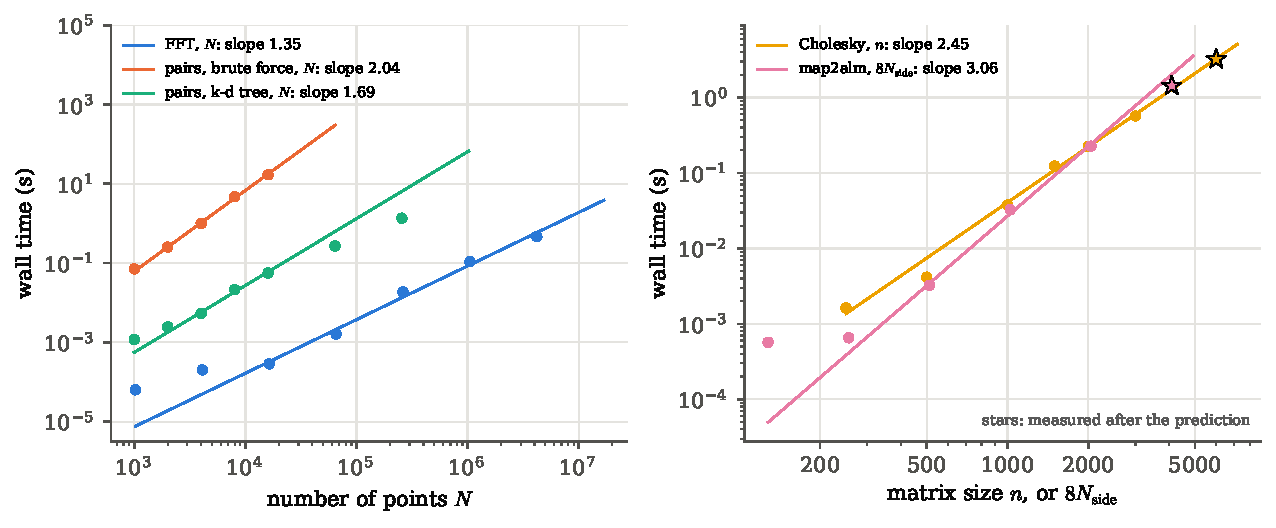
\includegraphics[width=\linewidth]{figures/chT0/10_cost.pdf}
\caption{Measured run times on one core (points) and power-law fits (lines), with the fitted exponents in the legends. Left: FFT, brute-force pair counting and $k$-d-tree pair counting against the number of points. Right: the Cholesky factor of an $n\times n$ matrix, and \texttt{map2alm} against $8N_{\rm side}$ (a rescaling that puts both on one axis). Stars: sizes beyond the fitted range, measured after the prediction was made.}
\label{T0a:fig:cost}
\end{figure}

What do the measured exponents say? Brute-force pair counting has slope $\TzSlopeBrute$, the counted $2$. \texttt{map2alm} has slope $\TzSlopeSht$ in $N_{\rm side}$, the counted $3$, and its prediction for $N_{\rm side}=512$, $\TzShtPred$\,s, compares with a measured $\TzShtMeas$\,s. The Cholesky fit predicts $\TzCholPred$\,s for $n=\TzCholBigN$ and the measurement is $\TzCholMeas$\,s. These are successes. Two exponents differ from the count, and both differences teach something. The FFT's slope is $\TzSlopeFft$, steeper than the $\TzFftNlogN$ that $N\log N$ alone would give over the same range: at the largest sizes the arrays no longer fit in the processor's fast cache memory, and every operation waits longer for its data. The Cholesky slope, $\TzSlopeChol$, is shallower than the counted $3$: for small matrices the fixed overheads are a large part of the time, and the optimised linear-algebra library also runs more efficiently on larger blocks, so the time grows more slowly than the operation count until the matrix is large. A fitted slope describes the range it was fitted on, and nothing guarantees it beyond.

\paragraph{Example: recalling the likelihood that cannot be evaluated.} \Cref{8a:sec:why-not-ml} asked how long one evaluation of the exact Gaussian likelihood of a CMB map would take. It needs the Cholesky factor of the $N_{\rm pix}\times N_{\rm pix}$ pixel covariance, and its script times that factor up to $n=6000$:

\pyfile[firstline=29,lastline=36,firstnumber=29]{code/ch08/03_cost_scaling.py}{The cost study of \cref{8a:sec:why-not-ml}: time at the largest size, exponent fixed by counting}

Lines 30--35 time the Cholesky factor of random positive-definite matrices, with the same best-of-three function as above. Line 36 is the instructive one: rather than fitting a slope, it fixes the exponent at the counted $3$ and uses only the largest, most nearly asymptotic, measurement to set the constant. From $\EightACholSix$\,s at $n=6000$ it predicted about $\EightALikeDaysTwoFiveSix$ days for the $786\,432$ pixels of $N_{\rm side}=256$, and $\EightAMemTwoFiveSix$\,TB of memory. The script of this section, on a single core, measured $\TzCholMeas$\,s at $n=6000$, about $\TzCholRatio$ times longer, because the earlier study let the linear-algebra library use up to four cores. With the counted exponent it predicts $\TzCholNsideDaysThree$ days, about $\TzDaysRatio$ times longer for the same reason: the two studies agree on the exponent and differ only in the constant. With its own fitted slope of $\TzSlopeChol$, however, it would predict only $\TzCholNsideDays$ days, an underestimate by more than a factor of ten, because a slope fitted where overheads still matter is extrapolated far beyond the range in which it was measured. When the asymptotic exponent is known by counting, use it, and take the constant from the largest size measured. Either way the conclusion of \cref{8a:sec:why-not-ml} stands: the exact pixel likelihood is out of reach, while a spherical-harmonic transform of the same map takes a fraction of a second.

\paragraph{Example: a Monte Carlo before it is run.} Suppose a study needs $1000$ simulated skies at $N_{\rm side}=256$, each analysed with three \texttt{map2alm} calls (temperature and two noise halves, say). One call took $\TzShtTwoFiveSix$\,s on one core, so the whole study needs about $3000\times\TzShtTwoFiveSix$\,s $\approx\TzMcMinutes$ minutes of transforms. That is within a laptop's budget on a few cores; at $N_{\rm side}=512$ it would be eight times longer, and at $N_{\rm side}=2048$, the resolution of the Planck maps, $512$ times longer, which is why the book's simulations stay at $N_{\rm side}\le512$ and say what the full-resolution version would cost. The grid evidence of \cref{5c:sec:grid-cost} is the same kind of estimate in a more dramatic form: an $n^4$ grid that takes $\FiveCGcTmax$\,s at $n=\FiveCGcNmax$ would take $\FiveCGcSixD$ years in six dimensions with a thousand points per axis.

\paragraph{The safety factor.} Extrapolation is uncertain in both directions: the exponent may change beyond the fitted range (the FFT and the Cholesky factor above), and a large run shares the computer with other work. A factor of two to three on the predicted time is prudent, and a prediction that is still uncomfortable after it is a prediction that the computation should not be run as planned. It should be made cheaper (a tree, an FFT, a coarser grid, an emulator), split over cores (\cref{T0a:sec:pool}), or sent to a bigger machine.

\begin{keyidea}[Estimate before you run]
Count how the work and the memory grow with the size of the problem; time the computation at a few small sizes; extrapolate with the counted exponent, the time measured at the largest size, and a safety factor of two or three. Anything that the estimate puts beyond about ten minutes or a few gigabytes is redesigned or moved to a bigger computer before it is started.
\end{keyidea}
\section{The whole toolkit on one page}
\label{T0a:sec:cheat}

\Cref{T0a:tab:cheat} is the toolkit in the order a script uses it: each concept, the smallest piece of syntax that does it, the subsection that explains it, and a place in the book where it does real work. The syntax column is meant to be read as a reminder of something already understood, not learned from.

\begin{table}[p]
\centering
\footnotesize
\renewcommand{\arraystretch}{1.12}
\begin{tabularx}{\linewidth}{@{}>{\raggedright\arraybackslash}p{2.75cm}
                               >{\raggedright\arraybackslash}X
                               >{\raggedright\arraybackslash}p{1.25cm}
                               >{\raggedright\arraybackslash}p{1.9cm}@{}}
\toprule
concept & syntax & here & at work in\\\midrule
\multicolumn{4}{@{}l}{\textbf{A script and plain Python}}\\
run a script & \texttt{python3 code/ch02/02\_binomial.py} & \S\ref{T0a:sec:anatomy} & \S\ref{2a:sec:binomial}\\
docstring, helpers & \texttt{"""Question: \dots"""}; \texttt{setup()}, \texttt{save\_numbers(\dots)} & \S\ref{T0a:sec:anatomy} & \S\ref{0a:sec:code}\\
f-string & \texttt{f"\{x:.3f\} \{n:,\} \{p:.2e\}"} & \S\ref{T0a:sec:strings} & \S\ref{1a:sec:events}\\
list, tuple & \texttt{xs = []}; \texttt{xs.append(v)}; \texttt{a, b = f(x)} & \S\ref{T0a:sec:containers} & \S\ref{3b:sec:newton}\\
dictionary & \texttt{d = \{"mean": m\}}; \texttt{for k, v in d.items():} & \S\ref{T0a:sec:containers} & \S\ref{3a:sec:sampling-python}\\
loops, conditions & \texttt{for i, v in enumerate(xs):}; \texttt{if \dots: elif \dots: else:} & \S\ref{T0a:sec:control} & \S\ref{1a:sec:events}\\
comprehension & \texttt{[f(v) for v in xs if v > 0]} & \S\ref{T0a:sec:control} & \S\ref{1b:sec:marginal}\\
function & \texttt{def f(x, n=10): return a, b}; \texttt{f(x, n=20)} & \S\ref{T0a:sec:functions} & \S\ref{3b:sec:invariance}\\
lambda & \texttt{lambda t: -loglike(t, data)} & \S\ref{T0a:sec:functions} & \S\ref{3b:sec:invariance}\\
import & \texttt{import numpy as np}; \texttt{from scipy import stats} & \S\ref{T0a:sec:imports} & every script\\
\midrule
\multicolumn{4}{@{}l}{\textbf{NumPy}}\\
array, shape, type & \texttt{x = np.array([1.0, 2.0])}; \texttt{x.shape}, \texttt{x.dtype} & \S\ref{T0a:sec:arrays} & \S\ref{1a:sec:events}\\
grids of numbers & \texttt{np.linspace(a, b, n)}; \texttt{np.logspace(p, q, n)} & \S\ref{T0a:sec:arrays} & \S\ref{1b:sec:pdf}\\
index, slice & \texttt{x[0]}, \texttt{x[-1]}, \texttt{x[a:b]}, \texttt{X[:, 0]}, \texttt{x[::-1]} & \S\ref{T0a:sec:indexing} & \S\ref{3a:sec:sampling-python}\\
mask & \texttt{x[(x > 0) \& (x < 1)]}; \texttt{np.mean(x > 2)} & \S\ref{T0a:sec:masks} & \S\ref{1a:sec:events}\\
broadcasting & \texttt{r[:, None] - r[None, :]}; \texttt{keepdims=True} & \S\ref{T0a:sec:broadcasting} & \S\ref{6b:sec:cholesky}\\
reduction & \texttt{X.mean(axis=1)}, \texttt{X.std(axis=0, ddof=1)} & \S\ref{T0a:sec:axis} & \S\ref{3a:sec:clt-python}\\
grids in $d$ dimensions & \texttt{np.meshgrid(x, y, indexing="ij")} & \S\ref{T0a:sec:grids} & \S\ref{7a:sec:phases}\\
random numbers & \texttt{rng = rng\_for("ch06", "name")}; \texttt{rng.standard\_normal(n)} & \S\ref{T0a:sec:random} & \S\ref{0a:sec:code}\\
linear algebra & \texttt{A @ x}; \texttt{np.linalg.solve(C, d)}; \texttt{cholesky}; \texttt{eigh} & \S\ref{T0a:sec:linalg} & \S\ref{6b:sec:cholesky}\\
Fourier transform & \texttt{np.fft.rfft(x)}; \texttt{np.fft.rfftfreq(n, dt)} & \S\ref{T0a:sec:fft} & \S\ref{9c:sec:pipeline}\\
\midrule
\multicolumn{4}{@{}l}{\textbf{SciPy, Matplotlib, files}}\\
distributions & \texttt{stats.norm.pdf}, \texttt{.cdf}, \texttt{.sf}, \texttt{.ppf}, \texttt{.logsf}, \texttt{.rvs} & \S\ref{T0a:sec:stats} & \S\ref{4a:sec:p-to-z}\\
integral & \texttt{val, err = integrate.quad(f, a, b)} & \S\ref{T0a:sec:quad} & \S\ref{1b:sec:marginal}\\
root & \texttt{optimize.brentq(f, a, b)} & \S\ref{T0a:sec:roots} & \S\ref{4b:sec:ci-intentions}\\
minimum & \texttt{res = optimize.minimize(f, x0)}; \texttt{res.x}, \texttt{res.success} & \S\ref{T0a:sec:minimize} & \S\ref{3b:sec:poisson-python}\\
log space & \texttt{special.gammaln(n + 1)}; \texttt{special.logsumexp(a)} & \S\ref{T0a:sec:logspace} & \S\ref{5c:sec:how-many}\\
figure & \texttt{fig, ax = plt.subplots()}; \texttt{ax.plot(x, y)}; \texttt{savefig(\dots)} & \S\ref{T0a:sec:matplotlib} & \S\ref{2a:sec:binomial}\\
files, cache & \texttt{np.savez(path, a=a)}; \texttt{np.load(path)}; \texttt{Path(\dots).exists()} & \S\ref{T0a:sec:files} & \S\ref{7b:sec:camb}\\
\midrule
\multicolumn{4}{@{}l}{\textbf{Seen a few times}}\\
data class & \texttt{@dataclass class Experiment: nside: int = 256} & \S\ref{T0a:sec:classes} & \S\ref{8a:sec:beam}\\
catching an error & \texttt{try: \dots{} except np.linalg.LinAlgError: \dots} & \S\ref{T0a:sec:try-with} & \S\ref{11c:sec:hubble-compare}\\
several cores & \texttt{with Pool(4) as pool: out = pool.map(f, jobs)} & \S\ref{T0a:sec:pool} & \S\ref{12c:sec:model}\\
compiled loop & \texttt{@njit} above a plain loop & \S\ref{T0a:sec:numba} & \S\ref{9b:sec:ising}\\
healpy, CAMB & \texttt{hp.alm2map}, \texttt{hp.anafast}; \texttt{camb.get\_results} & \S\ref{T0a:sec:blackbox} & \S\ref{7b:sec:camb}\\
\midrule
\multicolumn{4}{@{}l}{\textbf{Is it real? How long?}}\\
compare reals & \texttt{np.isclose(a, b)}; \texttt{abs(a / b - 1) < 1e-10} & \S\ref{T0a:sec:trust-float} & \S\ref{T2a:sec:dm}\\
Monte Carlo error & \texttt{x.std(ddof=1) / np.sqrt(len(x))} & \S\ref{T0a:sec:trust-mc} & \S\ref{0a:sec:code}\\
condition number & \texttt{np.linalg.cond(A)} & \S\ref{T0a:sec:trust-linalg} & \S\ref{8b:sec:invert}\\
more digits & \texttt{mp.mp.dps = 30}; \texttt{mp.mpf("1.01")} & \S\ref{T0a:sec:precision} & checks only\\
timing & \texttt{t0 = time.perf\_counter()} & \S\ref{T0a:sec:timing} & \S\ref{5c:sec:grid-cost}\\
\bottomrule
\end{tabularx}
\caption{The toolkit on one page. ``Here'' points to the subsection that explains it; ``at work in'' to a place where the book uses it on a real problem.}
\label{T0a:tab:cheat}
\end{table}

\paragraph{The census, once more.} The table has thirty-six rows. The census of \cref{T0a:sec:census} explains why that is enough. The book's $\TzFiles$ scripts make $\TzCalls$ calls to $\TzNames$ distinct library functions, but the calls are very unevenly shared: $\TzNfifty$ names make half of them, $\TzNeighty$ make $80\%$, and $\TzNninety$ make $90\%$. The other $\TzRareNames$ names are each used at most three times and together make only $\TzRareShare\%$ of the calls; each of those can be looked up in the documentation on the one occasion it is met. The syntax is more concentrated still: loops, function definitions, f-strings, slices, dictionaries and keyword arguments appear in most scripts, and classes, \texttt{try}, \texttt{while} and decorators in a few percent of them. A reader who knows the rows of \cref{T0a:tab:cheat}, and the habits of \cref{T0a:sec:trust,T0a:sec:precision,T0a:sec:cost}, can read every script in the book line by line, change it, and judge whether what it prints can be believed.

\section*{Chapter summary}
\addcontentsline{toc}{section}{Chapter summary}
\label{T0a:sec:summary}

Every number and figure in the book comes from a short script, and the scripts are written in a small, repetitive part of Python: a fixed anatomy, plain Python for the bookkeeping, NumPy for all arithmetic on arrays, a few SciPy tools, and a few Matplotlib calls. In the book's pipeline,
\[
  \text{physical model}\to\text{field or dataset}\to\text{summary }S\to P(S\given\theta)\to\text{infer physics},
\]
the code is the instrument that carries out every arrow, and the second half of the chapter is the instrument's calibration: what limits a computed number (rounding, the method, Monte Carlo noise), how to check each, when sixteen digits are not enough, and how to predict the cost of a computation before running it.

\begin{center}
\small
\renewcommand{\arraystretch}{1.15}
\begin{tabularx}{\linewidth}{@{}>{\raggedright\arraybackslash}p{3.2cm}
                               >{\raggedright\arraybackslash}X
                               >{\raggedright\arraybackslash}p{2.5cm}@{}}
\toprule
concept & operational meaning & used later in\\\midrule
the census & read every script's syntax tree without running it; count features, imports and calls; a few dozen names make most of the calls & every chapter\\
anatomy of a script & docstring (question, computes, writes), imports, settings, functions, computation and figure, numbers saved for the text & every chapter\\
vectorisation & one array expression instead of a Python loop; $\TzSpeedup$ times faster for a million elements & every chapter\\
broadcasting & arrays of different shapes combined by stretching axes of length one, compared from the right & \cref{ch:06,ch:07,ch:13}\\
seeded generator & \texttt{rng\_for(chapter, name)}: the same numbers on every run; streams for independent sequences & \cref{ch:06,ch:08,ch:09,ch:12}\\
solve, do not invert & $A^{-1}\bm b$ by \texttt{solve} or Cholesky; \texttt{inv} only when the inverse itself is wanted & \cref{ch:08,ch:10}\\
the seven traps & float equality, integer arrays, views, ranges, shapes, mutable defaults, missing seeds & every chapter\\
machine epsilon & $\epsilon=2^{-52}\approx2.2\times10^{-16}$, the relative spacing of \texttt{float64} numbers; compare with tolerances & \cref{ch:04,ch:10}\\
cancellation & subtracting nearly equal numbers multiplies the relative error by $(\abs a+\abs b)/\abs{a-b}$; rewrite the formula & \cref{ch:03,ch:04}\\
finite-difference step & central difference: best $h\sim\epsilon^{1/3}$, error $\sim\epsilon^{2/3}$; trust the plateau & \cref{ch:09,ch:10,ch:12}\\
condition number & $\kappa=\lambda_{\max}/\lambda_{\min}$; $\log_{10}\kappa$ digits lost; failed Cholesky means too few simulations or a singular matrix & \cref{ch:08,ch:10}\\
Monte Carlo error & $\sigma/\sqrt N$ quoted with every simulated number; common random numbers for differences & \cref{ch:06,ch:07,ch:08,ch:12}\\
convergence and validation & change the resolution until the answer stops moving; reproduce a known answer before trusting an unknown one & every chapter\\
decision rule & $z=\abs{\Delta}/\sqrt{\sigma_1^2+\sigma_2^2}$ with all errors; $z\gtrsim3$ is real (or a bug) & \cref{ch:04,ch:07}\\
log space and mpmath & \texttt{logsf}, \texttt{gammaln}, \texttt{logsumexp} first; mpmath at $d$ and $2d$ digits to check; trusted digits $\approx d-\log_{10}\kappa$ & \cref{ch:04,ch:05}\\
cost $O(N^p)$ & count the exponent, time small sizes for the constant, extrapolate with a safety factor; $8N^2$ bytes for an $N\times N$ matrix & \cref{ch:05,ch:08,ch:13}\\
\bottomrule
\end{tabularx}
\end{center}

\begin{recap}[Python for this book]
\begin{itemize}[leftmargin=1.2em,itemsep=1pt]
  \item The book's code uses a small vocabulary: $\TzNfifty$ names make half of all library calls and $\TzNninety$ make $90\%$. Learn those; look up the rest when they appear.
  \item A script reads like a derivation: question, imports, settings, computation, figure, numbers. Its numbers reach the text through \texttt{save\_numbers}, never by hand.
  \item NumPy does the arithmetic on whole arrays: shapes, slices, masks, broadcasting, reductions along an axis. Loops are kept for what is truly sequential.
  \item Randomness always comes from a seeded generator; matrices are solved, not inverted; real numbers are compared with tolerances.
  \item Every computed number has an error budget: rounding, the method, Monte Carlo noise. Check each by changing what controls it, validate on a known answer, and call a difference real only when it is large compared with the budget.
  \item Rewrite and use log space before asking for more digits; when asking, compare $d$ with $2d$.
  \item Count how the cost grows before running; time small sizes and extrapolate with a safety factor.
\end{itemize}
\end{recap}

\subsection*{Reading the literature}
\label{T0a:sec:reading}

\begin{itemize}[itemsep=2pt,leftmargin=1.2em]
  \item \textbf{The libraries.} The NumPy paper \cite{HarrisNumPy2020} explains the array model (shapes, strides, views, broadcasting, vectorised operations) on which everything here rests; the NumPy user guide, especially its pages on indexing, broadcasting and random generators, is the reference for exact behaviour. The SciPy paper \cite{VirtanenSciPy2020} describes the algorithms behind \texttt{quad} (QUADPACK), \texttt{brentq}, \texttt{minimize} and the distributions, and the SciPy reference guide gives every option and every returned field. Matplotlib is described in \cite{HunterMatplotlib2007}; its gallery is the quickest way to find how a particular kind of plot is drawn.
  \item \textbf{The physics libraries.} HEALPix is described in \cite{Gorski2005} and its Python interface healpy in \cite{ZoncaHealpy2019}; CAMB in \cite{CAMB2000}, with the CAMB Python documentation for the call pattern. numba is described in \cite{LamNumba2015}.
  \item \textbf{Floating point.} Goldberg's survey \cite{GoldbergFloat1991} is the classic account of how real numbers are stored and rounded, why cancellation happens, and how to rewrite formulas to avoid it. The mpmath documentation explains working precision (\texttt{mp.dps}) and the functions available at arbitrary precision.
\end{itemize}
  